\documentclass{article}
% Packages nécessaires

% Pour les documents en fran�ais...
	\usepackage[latin1]{inputenc}
	\usepackage[french]{babel}    
	\usepackage[french]{varioref} 
	
% Math�matiques
	\usepackage{amsmath}
	
% Caracteres speciaux
        \usepackage{latexsym,amsfonts}	

% A documenter	
	\usepackage{moreverb}
	\usepackage{lipsum}

% Pour ins�rer des graphiques	
%	\usepackage{graphicx}	% Graphique simples
	\usepackage{eso-pic,graphicx}	% Graphique simples    
	\usepackage{subfigure}				% Graphiques multiples
	\usepackage{xcolor}
	\usepackage{tikz}
%	\usepackage{animate}

% Pour le sch�ma de latex...
	%\usepackage[active,tightpage]{preview} 	
	%\PreviewEnvironment{tikzpicture}			
	%\setlength\PreviewBorder{5pt}					
	\usetikzlibrary{positioning}						
	
% Pour ins�rer des couleurs	
	\usepackage{color}

% Outil suppl�mentaire pour les tableaux
	\usepackage{multirow}
 	\usepackage{booktabs}
	\usepackage{longtable}
	\usepackage{colortbl}
	
% Rotation des objets et des pages
	\usepackage{rotating}
	\usepackage{lscape}

% Pour ins�rer du code source, LaTeX ou SAS par exemple.
	\usepackage{verbatim}
	\usepackage{fancyvrb}
	\usepackage{listings} 
	\lstset{language=SAS,numbers=left}		% Par d�faut le listing est en SAS 

% Pour ins�rer des hyperliens
	\usepackage{hyperref}

% American Psychological Association (for bibliographic references).
	\usepackage{apacite}
  
% Pour l'utilisation des macros
	\usepackage{xspace}

% Pour l'utilisation de notes en fin de document.
	\usepackage{endnotes}

% Rotation
	\usepackage{rotating}

% Pour les t�ches de caf�
	\usepackage{coffee}

% Symboles suppl�mentaires
	\usepackage{bbding}
	\usepackage{pifont}

% Pour les listes num�rot�es
%\usepackage{paralist}
	\usepackage{enumerate}
%\usepackage{enumitem}

% En t�tes et pieds de pages
 	\usepackage{fancyhdr}

% Pour le multi-colonne sous Beamer ?
	\usepackage{multicol}

% Pour la derni�re page
	\usepackage{lastpage}

% Pour Highlight d'Andre Simon
\usepackage{alltt}
%\usepackage[T1]{fontenc}

% Logos
\usepackage{mflogo}

%TikZ
  \usepackage{tikz}
  \usetikzlibrary{shadows,arrows}
  \pgfdeclarelayer{background}
  \pgfdeclarelayer{foreground}
  \pgfsetlayers{background,main,foreground}

% pour les symboles
\usepackage{keystroke}
%\usepackage{feyn}
\usepackage{bbding}
\usepackage{phonetic}
% Macros commandes

% Pour ins�rer des dessins de Linux
\newcommand{\LinuxA}{
\includegraphics[height=0.5cm]{Graphiques/linux.png}}
\newcommand{\LinuxB}{
\includegraphics[height=0.5cm]{Graphiques/linux.png}\xspace}

% Macro pour les petits dessins pour les diff�rents OS.
\newcommand{\Windows}{\emph{Windows}\xspace}
\newcommand{\Mac}{\emph{Mac OS X}\xspace}
\newcommand{\Linux}{\emph{Linux}\xspace}
\newcommand{\MikTeX}{MiK\tex\xspace}

% Des raccourcis pour les commandes \LaTeX, \TeX, ...
\newcommand{\latex}{\LaTeX\xspace}
\newcommand{\latexe}{\LaTeXe\xspace}
\newcommand{\tex}{\TeX\xspace}

% Commande pour le mode Verbatim
\newcommand{\code}{\vspace{0.2cm}\begin{Verbatim}[frame=single,label=Code,fontsize=\small]}
\newcommand{\tinycode}{\vspace{0.2cm}\begin{Verbatim}[frame=single,label=Code,fontsize=\tiny]}

% From Framabook (www.framasoft.net)
\newcommand{\latexcom}[1]{{\mdseries\ttfamily\upshape\symbol{92}#1}}
\newcommand{\indexcom}[1]{%
  \index{#1@\protect\texttt{\symbol{92}#1}}}
\newcommand{\ltxcom}[1]{%
  \latexcom{#1}\indexcom{#1}}  

  \newcommand{\yslant}{0.5}
\newcommand{\xslant}{-0.6}

% knitr
\usepackage[]{graphicx}\usepackage[]{color}
%% maxwidth is the original width if it is less than linewidth
%% otherwise use linewidth (to make sure the graphics do not exceed the margin)
\makeatletter
\def\maxwidth{ %
  \ifdim\Gin@nat@width>\linewidth
    \linewidth
  \else
    \Gin@nat@width
  \fi
}
\makeatother

\definecolor{fgcolor}{rgb}{0.345, 0.345, 0.345}
\newcommand{\hlnum}[1]{\textcolor[rgb]{0.686,0.059,0.569}{#1}}%
\newcommand{\hlstr}[1]{\textcolor[rgb]{0.192,0.494,0.8}{#1}}%
\newcommand{\hlcom}[1]{\textcolor[rgb]{0.678,0.584,0.686}{\textit{#1}}}%
\newcommand{\hlopt}[1]{\textcolor[rgb]{0,0,0}{#1}}%
\newcommand{\hlstd}[1]{\textcolor[rgb]{0.345,0.345,0.345}{#1}}%
\newcommand{\hlkwa}[1]{\textcolor[rgb]{0.161,0.373,0.58}{\textbf{#1}}}%
\newcommand{\hlkwb}[1]{\textcolor[rgb]{0.69,0.353,0.396}{#1}}%
\newcommand{\hlkwc}[1]{\textcolor[rgb]{0.333,0.667,0.333}{#1}}%
\newcommand{\hlkwd}[1]{\textcolor[rgb]{0.737,0.353,0.396}{\textbf{#1}}}%

\usepackage{framed}
\makeatletter
\newenvironment{kframe}{%
 \def\at@end@of@kframe{}%
 \ifinner\ifhmode%
  \def\at@end@of@kframe{\end{minipage}}%
  \begin{minipage}{\columnwidth}%
 \fi\fi%
 \def\FrameCommand##1{\hskip\@totalleftmargin \hskip-\fboxsep
 \colorbox{shadecolor}{##1}\hskip-\fboxsep
     % There is no \\@totalrightmargin, so:
     \hskip-\linewidth \hskip-\@totalleftmargin \hskip\columnwidth}%
 \MakeFramed {\advance\hsize-\width
   \@totalleftmargin\z@ \linewidth\hsize
   \@setminipage}}%
 {\par\unskip\endMakeFramed%
 \at@end@of@kframe}
\makeatother

\definecolor{shadecolor}{rgb}{.97, .97, .97}
\definecolor{messagecolor}{rgb}{0, 0, 0}
\definecolor{warningcolor}{rgb}{1, 0, 1}
\definecolor{errorcolor}{rgb}{1, 0, 0}
\newenvironment{knitrout}{}{} % an empty environment to be redefined in TeX


% Commandes vari�es
\newcommand{\df}{\emph{data.frame}\xspace}
\newcommand{\liste}{\emph{list}\xspace}
\newcommand{\cad}{c'est-�-dire\xspace}
\newcommand{\Rcode}{code \includegraphics[height=0.75em,width=1em]{logo_R}}
\newcommand{\Sweave}{\emph{Sweave}\xspace}
\newcommand{\knitr}{\emph{knitr}\xspace}

 % Définition de l'auteur, ...
% Titre  	 
        \title{Introduction � \LaTeX}
        \author{Pascal Bessonneau}
	\date{05/2016}

% Pieds de page, marges, ...
% page layout

% By LaTeX commands
%\setlength{\oddsidemargin}{0cm}
%\setlength{\textwidth}{16cm}
%\setlength{\textheight}{24cm}
%\setlength{\topmargin}{-1cm}
%\setlength{\marginparsep}{0.2cm}

% fancyheader parameters
%\pagestyle{fancy}  

\fancyfoot[L]{{\small Formation \LaTeX, DEPP}}
\fancyfoot[c]{} 
\fancyfoot[R]{{\small \thepage/\pageref{LastPage}}}

\fancyhead[L]{} 
\fancyhead[c]{}
\fancyhead[R]{} 

\begin{document}
\maketitle
\newpage
\tableofcontents
\newpage
\section{L'histoire en trois mots...}

      \subsection{L'histoire en trois mots...}

			A l'origine de \latex, il y a un homme, Donald Knuth. Math�maticien et informaticien de g�nie, il est l'auteur de plusieurs ouvrages de r�f�rence dont \emph{The Art of Computer Programming}.
			
			Il a con�u non pas \latex mais \tex. \tex est venu, � la fin des ann�es 70, de l'amour de la typographie et des beaux documents de Knuth. 
			
			Knuth est �galement le concepteur de \emph{Metafont}~: c'est un langage permettant de faire des dessins qui s'incorporent naturellement avec \tex. Le langage est un peu difficile mais les r�sultats sont spectaculaires.


			
				Dans un second temps, \tex �tant un peu trop aride, Leslie Lamport a d�velopp� \latex qui se superpose � \tex et qui offre une syntaxe plus conviviale. 

				Mais en fait \latex n'a pas �t� la seule extension de \tex, \tex a donn� naissance a plusieurs b�b�s... Parmi les plus c�l�bres~:  

				\begin{itemize}
					\item \latex, \latexe
					\item \href{http://www.pragma-ade.nl/}{Con\tex}\footnote{http://www.pragma-ade.nl/}
					\item \href{http://scripts.sil.org/cms/scripts/page.php?site_id=nrsi&id=xetex}{Xe\tex}\footnote{http://scripts.sil.org/cms/scripts/page.php?site \_ id=nrsi \& id=xetex}
					\item ...
				\end{itemize}
				
    	

			Ils ont tous en commun \tex mais leurs langages et leurs possibilit�s varient un peu. 
			
			Le plus portable est \latex. Un concurrent tr�s s�rieux est \href{http://www.pragma-ade.nl/}{Con\TeX} qui permet facilement de faire des choses peu ais�es � r�aliser en \latex.
			
			\href{http://scripts.sil.org/cms/scripts/page.php?site_id=nrsi&id=xetex}{Xe\tex} quant � lui permet d'utiliser une gestion des caract�res et des fontes tr�s avanc�es (notamment les ligatures).




\section{Qu'est ce que \latex ?}
 
      \subsection{Un langage de mise en forme...}
      
      \TeX est un langage informatique qui permet la mise en page de document. 
      
      Par opposition au logiciel \og~What You See Is What You Get~\fg tels que Word, le principe de \TeX est de fournir � un compilateur un fichier texte contenant le texte et les commandes de mises en forme � ex�cuter sur ce texte.
      
      Tr�s grossi�rement, \latex peut se comparer � de l'HTML~: un m�lange de texte et de \og~balises~\fg. 


      \subsection{Un petit exemple de code \latex}

\tinycode
	\subsection{Un langage de mise en forme...}
      
  \TeX est un langage informatique qui permet la mise en page de document. 
      
  Par opposition au logiciel \og~What You See Is What You Get~\fg tels que Word, le principe de 
  \TeX est de fournir � un compilateur un fichier texte contenant le texte et les commandes de 
  mises en forme � ex�cuter sur ce texte.
      
  Tr�s grossi�rement, \latex peut se comparer � de l'HTML~: un m�lange de texte et de 
  \og~balises~\fg. 

\end{Verbatim}
      
      \subsection{Phases pour la production d'un document}

			\begin{enumerate}
				\item L'utilisateur r�alise le fichier \og~.tex~\fg
				\item l'utilisateur lance le compilateur sur le fichier \og~.tex~\fg 
				\item Le compilateur renvoie le cas �ch�ant les erreurs de compilation
				\item En l'absence d'erreurs, le compilateur produit le fichier PDF ou PostScript
      \end{enumerate}
      


\section{Avantages et inconv�nients}
  
      \subsection{Les avantages de \latex}
      
      \latex permet de concentrer l'effort du r�dacteur sur le contenu et non sur la mise en forme~: la mise en forme d�coule directement du plan du document.  
      
      Le rendu est assez unique et permet d'obtenir des documents extr�mement propres notamment pour les fonctions math�matiques. 
      
      Les logiciels sont disponibles sur pratiquement toutes les plateformes existantes : \Windows, \Mac, \Linux, \emph{Solaris}, ...



			Comme c'est un langage de programmation, le rendu correspond exactement � ce que l'utilisateur a sp�cifi�.  
						
			Comme c'est un langage il est possible de~:
			\begin{itemize}
				\item reproduire fid�lement un document (depuis un mod�le de document par exemple)
				\item transmettre le document brut qui se compilera sur n'importe quelle plateforme de la m�me fa�on
				\item automatiser les processus
				\item ...
			\end{itemize}



			Et il y'a les maths... \'Ecrit par un math�maticien, �crire des maths en \latex est rapide et confortable.
			
			Et c'est un logiciel libre~:) Donc gratuit, maintenu par une communaut� de programmeurs actives, documentation abondante sur Internet, ... 


      \subsection{Les inconv�nients de \latex}

			\begin{itemize}
				\item \latex est un langage et n�cessite donc un apprentissage
				\item changer radicalement la pr�sentation par rapport aux pr�sentations par d�faut est une t�che parfois lourde
				\item \latex repose sur des fichiers texte ce qui suppose quelques acrobaties entre les formats de fichiers texte (Latin1, ISO, UTF-8, ...) 
			\end{itemize}		


\section{Comment faire du \latex ?}

      \subsection{Sur le principe...}

				Le fichier texte peut �tre cr�� et/ou modifi� par n'importe quel �diteur de texte. 
				
				Puis dans l'interpr�teur de ligne de commande, vous appelez un des compilateurs~: 
				\begin{description}
					\item [latex,dvips] pour passer du fichier texte au fichier PostScript
					\item [pdflatex] pour passer du fichier texte au fichier PDF
				\end{description}

				Le nom du compilateur peut varier selon les plates-formes et la version de \latex utilis�e.

    	    	

				Pour un fichier texte \emph{monfichier.tex}, cela donnerait dans l'interpr�teur ligne de commande sous Windows (Mik\TeX)~:
\code
pdflatex monfichier.tex
\end{Verbatim}				

			pour obtenir depuis le fichier \og~monfichier.tex~\fg le fichier PDF correspondant.

    	
      \subsection{En vrai...}

			Les fichiers \latex ne s'�ditent pas avec le bloc-notes de \Windows... 
			
			Des �diteurs beaucoup plus conviviaux sont disponibles pour cr�er et modifier des fichiers \latex. Ils permettent d'�diter confortablement les fichiers et de compiler les fichiers sans passer par un interpr�teur de commande.


      \subsection{Les �diteurs de texte intelligents}

			Pourquoi utiliser ces �diteurs plut�t que le bloc-note ?
			\begin{itemize}
				\item Ils permettent de diff�rencier visuellement les commandes \latex du texte \og~brut~\fg
				\item Ils permettent de ne pas passer par la console pour compiler
				\item Ils apportent une aide (raccourcis, g�n�ration de code \latex, ...) lors de l'�dition
				\item Beaucoup d'entre d'eux permettent d'utiliser et/ou de modifier l'encodage

			\end{itemize}
			
			Des �diteurs beaucoup plus conviviaux sont disponibles pour cr�er et modifier des fichiers \latex.


\section{Les �diteurs am�lior�s pour \latex}

      \subsection{En vrai...}

				Les �diteurs sont parfois appel�s �galement environnements de d�veloppement int�gr�s (IDE). 
				
				Quelques exemples...
				\begin{itemize}
					\item \href{http://www.xm1math.net/texmaker/}{\TeX Maker}
					\item \href{http://www.tug.org/texworks/}{\TeX Works} (toutes plates formes)
					\item	\href{http://www.texniccenter.org/}{\TeX nicCenter} Windows
					\item	\href{https://www.gnu.org/software/emacs/}{Emacs} (toutes plates formes)
					\item ...
				\end{itemize}
				
    	    	
      	\subsection{\href{http://www.xm1math.net/texmaker/}{\TeX Maker}}
      	
			\TeX Maker est tr�s bien. Lorsque vous compilez de \latex en Postscript, il fait appara�tre le log et surtout les erreurs de compilation de fa�on tr�s claire.
			
			Il supporte les formats Latin1 et Unicode ce qui est plut�t bien pour \Windows et \Mac. En effet, dans les pr�f�rences, on peut d�finir le type d'encodage que l'on souhaite utiliser.
			
    	    	
      	\subsection{\href{http://www.tug.org/texworks/}{\TeX Works}}

			\TeX Works est similaire � \TeX Maker avec quelques fonctionnalit�s suppl�mentaires. 
			
			Une version portable, sans installation est disponible sur le site.


      	\subsection{\href{http://www.texniccenter.org/}{\TeX nicCenter}}

			\TeX nicCenter a un gros avantage c'est qu'il compile la totalit� du fichier \latex m�me en pr�sence d'erreurs... C'est le plus riche en mati�re de personnalisation de la compilation. 
			
			Il ne corrige pas vos fautes, mais vous permet de regarder en une seule passe s'il y a une ou plusieurs erreurs dans votre fichier \latex~: il suffit d'appuyer sur \emph{F9} et vous passez d'une erreur � l'autre tout au long du fichier log. C'est tr�s pratique. 
			
			En revanche, il ne supporte pas les fichiers Unicode ce qui peut poser probl�me.


\section{Compiler un document \latex sur son poste de travail}

      \subsection{Oui mais le compilateur ?}

				Pour compiler un document \latex sur votre poste de travail, vous avez la possibilit� d'utiliser une version portable ou, si vous avez les droits administrateurs sur votre poste, d'installer une \og~distribution~\fg.
				
				Une distribution installe de nombreux compilateurs, logiciels, packages et modifie les valeurs syst�me pour permettre une utilisation optimale de \latex.

    	
      \subsection{FramaKey, Paquet \latex}
    	
				La premi�re possibilit� est la \href{http://framakey.org/Pack/PackLatex}{FramaKey}\footnote{http://framakey.org/Pack/PackLatex}. C'est une version portable. Elle ne n�cessite aucune installation et n'exige pas que vous soyez administrateur de votre poste. 
    	
    	Il suffit de d�-zipper le fichier t�l�charg� sur le site de Framasoft. Les utilitaires et les compilateurs minimaux sont pr�sents et correctement configur�s.
			
			{ \bfseries La Framakey \latex n'est pas tr�s bien mise � jour. Le r�sultat est qu'il est difficile de s'en servir car les paquets correspondant � la version de \latex sur la clef n'existe plus en ligne.
			
			La FramaKey est donc � �viter pour l'instant \dots }


      \subsection{\MikTeX, version portable}
    	
				La version portable de \MikTeX permet de r�aliser des documents \latex. Elle ne n�cessite ni droits administrateurs ni installation comme la FramaKey.
    	
    	Il suffit de d�-zipper le fichier t�l�charg� sur le site de Framasoft. Les utilitaires et les compilateurs minimaux sont pr�sents et correctement configur�s. La page indique comment utiliser la version portable. Notamment le lancement de l'environnement avec la petite application dans la barre des t�ches.
			
			Le fichier est t�l�chargeable \href{http://miktex.org/portable}{\textcolor{blue}{ici}}.


      \subsection{Les distributions}

				La seconde possibilit� est d'installer une distribution. Les distributions les plus communes par plate-formes sont~:
				
				\begin{itemize}
					\item{\Windows} \href{http://www.tug.org/mactex/}{\MikTeX}
					\item{\Mac} \href{http://www.tug.org/mactex/}{MacTeX}
					\item{\Linux}	\href{http://www.tug.org/texlive/}{TeXLive}
				\end{itemize}
				

      \subsection{\MikTeX}

				L'installation de \MikTeX, r�serv�e aux administrateurs de leur poste. Par cons�quent elle ne sera pas d�crite ici. Sur demande, un document d'aide est toutefois fourni avec les documents du cours.
							
    	
% Ins�rer un glossaire %
    	
\section{Les parties du code}

      	\subsection{Structure d'un fichier \latex}

				\latex est un langage � balise qui n'est pas sans rappeler HTML. 
				
				Comme HTML, il y a une premi�re partie, en amont du texte qu'on appele \textit{preambule}. Il correspond au \emph{header} de l'HTML. 
				
				Apr�s une commande \latex sp�cifique, la seconde partie du document commence~: c'est le corps du document contenant ce qui va �tre lisible dans le document final.
				
				Puis une commande \latex termine le document.

				
				
				La d�finition minimale d'un document \latex est~:
				
\code
\documentclass{article}
...
...
\end{Verbatim}
				

      \subsection{Le pr�ambule}

\code
\documentclass{article}
\usepackage[latin1]{inputenc}
\usepackage[french]{babel}
\title{Introduction � \latex}
\author{Pascal Bessonneau}
\date{DEPP, 12/2010.}
\definecolor{myblue}{rgb}{0,0.31,0.64}
\renewcommand\section{\@startsection {section}{1}{\z@}%
	{-3.5ex \@plus -1ex \@minus -.2ex}%
	{2.3ex \@plus.2ex}
\end{Verbatim}



				Le pr�ambule va contenir~: 			
				\begin{enumerate}
					\item	La liste des paquets que doit charger \latex
					\item La d�finition ou la red�finition des couleurs
					\item La d�finition ou la red�finition des commandes
					\item	Les informations concernant le titre, l'ouvrage, ...					
					\item ...
				\end{enumerate}
				

				\subsection{Le corps du document}
			
				Dans cette partie, sauf exception, le texte va �tre compil� et va apparaitre dans le document.
				
				Cette partie est d�finie par les commandes~: 			
				
\code
...
\maketitle
...
La preuve qu'il y a des �tres intelligents...
essay�s de nous contacter.
...
\ end{document}
\end{Verbatim}				
			

				\subsection{\latex est un langage...}
				
				\latex est un langage proche d'un langage de programmation par cons�quent il faut respecter des conventions simples~:
				\begin{itemize}
					\item pour que le compilateur \latex puisse interpr�ter correctement les commandes
					\item pour vous faciliter le travail de recherche et corrections des erreurs
					\item pour faciliter la vie du(des) relecteur(s) du code
				\end{itemize}					
				

				
				Par cons�quent on retiendra les r�gles suivantes~: 
				\begin{itemize}
					\item toutes les commandes \latex sont � taper en minuscules (en fait c'est une obligation \latex est sensible � la casse)
					\item � l'int�rieur et � l'ext�rieur du document, ne pas h�siter � laisser des espaces ou des tabulations pour augmenter la lisibilit�
					\item ajouter des commentaires pertinents pour la relecture ou le d�bogage
				\end{itemize}
				

\section{Les packages}
							
      \subsection{Les packages}

	    	Les paquets (ou \emph{packages}) sont un ensemble de macro-commandes. Ils sont un peu � l'image des macros INSEE de SAS ou des paquets de R.
	    	
	    	Ces macros permettent de r�aliser des mises en pages avanc�es, de changer la langue du document, de cr�er des tableaux personnalis�s, ...
	    	
	    	Ces ensembles de commandes \tex et/ou \latex permettent de r�aliser des op�rations sur le document ou les donn�es associ�es.
	    	
	    	Vous devez les appeler dans le pr�ambule. 
	    	
	    
	
	    	Les paquets sont au nombre de quelques milliers. Le probl�me est souvent de trouver le paquet qui fait ce que l'on souhaite. 
	    	
	    	Les paquets officiels (stables) sont disponibles sur le site \href{http://www.ctan.org/}{Comprehensive \tex~Archive Network}.
    	    	
			

				Lors de l'installation sous \Windows avec Mik\tex, on peut installer (presque) l'ensemble des paquets (ce qui repr�sente 1,2 Go).
				
				Sinon on peut les installer � la demande... Si vous utilisez un paquet non pr�sent sur l'ordinateur, l'�diteur \latex vous proposera automatiquement (avec le bon r�glage) de l'installer.
    	    	

    	\subsection{Le paquet \textit{inputenc}}
    	
    	A retenir et � placer dans tous vos documents~: 
    	
\code    	
\usepackage[latin1]{inputenc}
\end{Verbatim}

\code    	
\usepackage[utf8]{inputenc}
\end{Verbatim}

Le paquet \emph{inputenc} permet de d�finir le format de fichier texte (Latin1, UTF-8, ...). Il est important car il permettra � \latex de reconnaitre notamment les caract�res accentu�s.
			

    	\subsection{Le paquet \textit{babel}}
    	
    	A retenir et � placer dans tous vos documents r�dig�s en fran�ais~: 
    	
\code    	
\usepackage[french]{babel}
\end{Verbatim}

			Le paquet Babel permet de \textit{franciser} les guillemets, les c�sures, les accents, ... 
						
		
    	\subsection{Un package tout � fait inutile}
    	
    	Nous verrons des packages utiles mais voil� un exemple de package tout � fait inutile donc indispensable~: \latex Coffee Stains
    	
    	\cofeAm{1}{0.5}{0}{2.5cm}{0cm}
    				

\section{L'encodage des caract�res}

      \subsection{L'encodage des caract�res en quelques mots...}

	L'encodage des caract�res provient du conflit entre les limites qui �taient impos�es par les ordinateurs et la diversit� des alphabets et des glyphes utilis�s dans chaque langue.

Ainsi, les premiers jeux de caract�res cod�s sur peu de bits ne contenait pas les caract�res accentu�s. Puis le codage des caract�res a �t� r�alis� sur un plus grand nombre de bits, offrant la possibilit� de coder (presque tous) les caract�res d'une langue.

Et ainsi de suite jusqu'� parvenir aux syst�mes actuels qui permettent le codage d'un grand nombre de glyphes.

    	   	

ANSI, ISO-8859-x, Unicode... sont autant de normes utilis�es pour repr�senter les caract�res d'une langue.

Aujourd'hui, si \Windows XP et certains logiciels utilise la norme ISO \textit{Western character}, ie. ISO-8859-1,  la plupart des syst�mes d�cents utilise l'Unicode.

Unicode, plus r�cent et offrant un tr�s large panel de caract�res, est � pr�f�rer. Seul b�mol, Unicode est d�riv� en 8bits, 16bits et 32bits. 



Pourquoi parler de l'encodage ? La raison est qu'il faudra lors des �changes de fichiers s'assurer d'utiliser le m�me encodage sous peine de voir des caract�res exotiques ou des erreurs de compilation appara�tre.

L'autre exemple type est le copier-coller. Le copier-coller de Word dans une �diteur de texte peut s'av�rer probl�matique. 


      \subsection{Indiquer � \latex d'utiliser un autre format d'encodage}
				
				Il suffit de pr�ciser l'encodage en d�but de document (le pr�ambule)~:
\code
\usepackage[latin1]{inputenc}
\end{Verbatim}

			Ici l'encodage est en \emph{latin1} (ISO-8859-1). \emph{utf8}) correspond � Unicode (UTF8).
				

      \subsection{La conversion de fichier texte}
				
				Des utilitaires comme \href{http://notepad-plus-plus.org/}{Notepad++} peuvent vous permettre de convertir le texte d'un format � l'autre. 
				
				Sinon des langages de programmation comme R, Perl et Python permettent de le faire �galement.
				
				Pour faire de l'aide sur ce point, le terme exacte est translitt�ration plut�t que conversion.
				




\section{Le langage \latex}
				
  	\subsection{Le langage}

			\latex utilise des caract�res sp�ciaux que le compilateur va reconnaitre et utiliser pour baliser le texte.
			
			Ainsi les caract�res \textbackslash, \$, \&, \_, \{, \}, \%, [, ], \textasciitilde\ sont r�serv�s. Ils ont une signification particuli�re. 

			Par exemple~:
			\begin{center}
				\textbackslash commande [ \emph{options} ] \{ \emph{argument} \}
			\end{center}

			\emph{commande} va �tre reconnue comme une commande ou macro-commande \latex.
			

    	
    	Quand la commande prend un argument obligatoire, la syntaxe devient~:
    	
			\begin{center}
				\textbackslash commande\{ \emph{argument} \}
			\end{center}
			
			
    	Quand la commande prend plusieurs arguments obligatoires, la syntaxe devient~:
    	
			\begin{center}
				\textbackslash commande\{ \emph{argument1} \}\{ \emph{argument2} \}...
			\end{center}
			


    	
    	Lorsque qu'un argument est optionnel alors il est entre crochets~:
    	
			\begin{center}
				\textbackslash commande [ \emph{options} ] \{ \emph{param�tre} \}
			\end{center}

			L'ajout d'une * permet dans certains cas de modifier un peu le comportement d'une fonction.
	
		

			Un document \latex tr�s simple~:
			
\code
% Document 01
\documentclass{article}
\usepackage[latin1]{inputenc}
\usepackage[french]{babel}
\title{Introduction � \latex}
\author{Pascal Bessonneau}
\date{DEPP, 12/2010.}
\maketitle
La preuve qu'il y a des �tres intelligents...
\end{Verbatim}			
			

  	\subsection{Les environnements}
		
	Les environnements vont �tre d�finis comme suit~:
			
\code
\begin{nom}
...
\end{nom}
\end{Verbatim}


		
			Les types d'environnements sont nombreux en \latex~: listes, code source, \dots\ Ils permettent de sp�cifier un ensemble de propri�t�s pour les objets � l'int�rieur de l'environnement.

			Ils commencent par un \textbackslash begin et se termine par un \textbackslash end suivi dans les deux cas par le type d'environnement.
						
		
  	\subsection{Les groupes}

			Une syntaxe l�g�rement diff�rente permet de d�finir des groupes. Cette syntaxe se rapproche de celle de R ou Perl~:
			
\code
{ \mot-clef
...
}
\end{Verbatim}

			Ce type de syntaxe se retrouve notamment pour les changements de police.
						

  	\subsection{Les caract�res r�serv�s}

		En plus des caract�res r�serv�s vus pr�c�demment, ils existent d'autres caract�res ayant une signification pour \latex comme le @ par exemple. Ils sont utilis�s par \latex pour l'appel de variables priv�es, les maths, \dots

		Dans le tableau \ref{car:reserves}, la liste des correspondances pour ces caract�res est donn� pour les inclure en tant que tel dans un texte.
		
		\begin{center}
			\begin{figure}
				\scalebox{0.8}{
				\begin{tabular}{ccl}
					{ \bf Caract�re } & { \bf Fa�on de l'�crire en \latex } & { \bf Fonction }\\
					\hline
					\$ & \textbackslash\$ & sert pour  les math�matiques\\
					\& & \textbackslash\& & sert pour les tableaux et les maths\\
					\_ & \textbackslash\_ & sert en mode math�matique\\
					\{ & \textbackslash\{ & sert pour les appels de fonction\\
					\} & \textbackslash\} & sert pour les appels de fonction\\
					$[$ & $[$ & sert pour les appels de fonction\\
					$]$ & $]$ & sert pour les appels de fonction\\
					\% & \textbackslash\% & lance le mode commentaire\\
				\end{tabular}}
			\end{figure}
		\end{center}
		
		
  	\subsection{Les caract�res accentu�s}

		Les caract�res accentu�s sont g�r�s par \latex en sp�cifiant correctement l'encodage des caract�res. Toutefois pour les majuscules accentu�esil suffit pour le fran�ais d'utiliser les commandes suivantes~:
		
		\begin{center}
			\begin{tabular}{cc}
				Accents et graph�mes & code \latex\\
				\'E & \textbackslash'E\\
				\`E & \textbackslash`E\\
				\^A & \textbackslash\textasciicircum a\\
				\"I & \textbackslash"I\\
				\c C & \textbackslash c\ C\\
				c\oe ur & c\textbackslash oe\ ur\\
				C\OE ur & C\textbackslash OE\ UR\\
				\ae & \textbackslash ae\\
				\AE & \textbackslash AE\\
			\end{tabular}
			
		\end{center}
		

		
		Pour une liste exhaustive des commandes disponibles, cette \href{http://www.tuteurs.ens.fr/unix/accents.html}{page} est tr�s bien faite. 
		
		Ces commandes fonctionnent �galement pour les minuscules. Ceci est int�ressant de le savoir notamment dans le cas o� l'encodage est impos� comme les fichiers bibtex (r�f�rences bibliographiques).
				
				
  	\subsection{Les caract�res sp�ciaux}

		\href{http://www.tex.ac.uk/tex-archive/info/symbols/comprehensive/symbols-a4.pdf}{The Comprehensive \latex~Symbols list} est un document pr�cieux... Il contient tous les caract�res sp�ciaux accessibles y compris dans certains paquets comme \emph{amsmath}. 
		
		Il y en a plusieurs milliers~: 
		\copyright, 		\textdagger, 		\emgma, 		\AltGr, 		\Checkmark, 		\SnowflakeChevron, 		\dots		

  	\subsection{La gestion des espaces et des tabulations}

			Les espaces sont automatiquement g�r�s par le compilateur qui supprime les espaces et les tabulations exc�dentaires~: 
\code
La preuve qu'il y a des �tres...\\							
La         preuve         qu'il y a des  �tres...\\
\end{Verbatim}
			
			donne\\
			
La preuve qu'il y a des �tres...\\							
La         preuve         qu'il y a des  �tres...\\

		
  	\subsection{Sauts de ligne et commentaires}

		Quand vous laissez une ligne blanche, \latex suppose que vous passez au paragraphe suivant. Un paragraphe correspond donc � un blocs de lignes sans lignes vides. 
		
		En cas de besoin, vous pouvez forcer un saut de ligne en utilisant la commande \textbackslash\textbackslash comme dans l'exemple pr�c�dent.

		Des commentaires peuvent �tre ajout�s en d�but de ligne ou plus loin... Tout ce qui suit un \% est un commentaire.


\section{Type de document}
 
      \subsection{documentclass}

				Le \emph{documentclass} va donner l'allure g�n�rale du document~: 
				\begin{itemize}
					\item article~: pour les articles scientifiques, les pr�sentations, les rapports courts, la documentation de programme, les invitations,...
					\item proc~: une classe pour les actes de conf�rences bas� sur \emph{article}
					\item minimal~: Il contient seulement les r�glages pour la dimension de la page et une police de base. Il est con�u plut�t pour du d�boguage
					\item report~: pour les rapports plus longs contenant quelques chapitres, les petits livres, les th�ses, ...
					\item book~: pour les livres
					\item slides~: pour les diapositives. La classe utilise des grandes lettres sans serif
					\item memoir~: pour changer sensiblement la pr�sentation du document. Ce type est bas� sur le type \emph{book} mais vous pouvez cr�er n'importe quel document avec
					\item letter~: pour les lettres
				\end{itemize}					
				


				Il existe d'autres \emph{documentclass} d�velopp�s et qui sont disponibles sous forme de paquets ou de fichiers de styles~:
				\begin{itemize}
					\item Beamer, pour les pr�sentations
					\item Prosper, idem
					\item Mod�le de revue (ex: \emph{Journal of Statistical Software})
					\item ...
				\end{itemize}
			

      \subsection{Les mots-clefs}

			Associ� au \emph{documentclass}, des mots-clefs permettent de remplir des champs pr�d�finis~: auteur, titre, date, ...
			
			Attention, les mots-clefs pr�d�finis d�pendent du type de \emph{documentclass} que vous utilisez. Ils permettront d'une part de cr�er les titres et d'autre part de renseigner les champs des fichiers PDF cr��s. 

			Il faut m�moriser la fa�on dont les renseignements sont entr�s qui est classique sous \latex~: 
			\begin{center}
				\textbackslash commande \{ \emph{param�tre} \}
			\end{center}

    	
  	\subsection{La structuration des documents}

			il est plus difficile dur d'�crire un document non structur� avec \latex. En effet vous pouvez jouez un peu avec la typographie mais en fait la mise en forme des titres passe par une commande qui d'une part~: 
			\begin{itemize}
				\item	mets la mise en forme adapt�e au niveau hi�rarchique
				\item ajoute une r�f�rence dans la table d'index afin de l'inclure dans la table des mati�res
			\end{itemize}


  	\subsection{La structuration~: book}
  	
  	Les niveaux hi�rarchiques d�finis par d�faut sont~:
  	\begin{itemize}
			\item \textbackslash part\{\}
			\item \textbackslash chapter\{\}
			\item \textbackslash section\{\}
			\item \textbackslash subsection\{\}
			\item \textbackslash paragraph\{\}
			\item \textbackslash subparagraph\{\}
		\end{itemize}			
			

  	\subsection{La structuration~: report}
  	
  	Les niveaux hi�rarchiques d�finis par d�faut sont~:
  	\begin{itemize}
	  	\item \textbackslash part\{\}
	  	\item \textbackslash chapter\{\}
	  	\item \textbackslash section\{\}
	  	\item \textbackslash subsection\{\}
	  	\item \textbackslash paragraph\{\}
	  	\item \textbackslash subparagraph\{\}
  	\end{itemize}			
			

  	\subsection{La structuration~: article}
  	
  	Les niveaux hi�rarchiques d�finis par d�faut sont~:
  	\begin{itemize}
			\item \textbackslash part\{\}
			\item \textbackslash section\{\}
			\item \textbackslash subsection\{\}
			\item \textbackslash paragraph\{\}
			\item \textbackslash subparagraph\{\}
  	\end{itemize}			
			

  	\subsection{La structuration~: letter}
			
			La structure est un peu diff�rente et on ne retrouve que les commandes suivantes~: 
			\begin{itemize}
				\item \textbackslash signature\{\}
				\item \textbackslash address\{\}
				\item \textbackslash opening\{\}
				\item \textbackslash closing\{\}
			\end{itemize}					
		

  	\subsection{La table des mati�res}
  	
  	Une fois que le document contient la structure, il suffit de taper la commande...
\code    
\tableofcontents  	
\end{Verbatim}
...~pour imprimer la table des mati�res o� on le souhaite.

		
  	\subsection{Eviter le r�f�rencement}
  	
  	Si on ne veut pas qu'une \emph{section}, \emph{chapter}, ...  apparaisse dans la table des mati�res il faut utiliser une *~:

\code    
\section*{Mon titre de section}
\end{Verbatim}  	
  	
  	Ce titre apparaitra dans le m�me style qu'un titre de section classique mais pas dans la table des mati�res.
  	

\section{La compilation}
		
  		\subsection{La compilation...}
  	
  		Entre le fichier texte et le fichier final, il y a une phase de compilation.
  		
  		Le principe est que le fichier va �tre interpr�t� puis traduit au format PostScript ou PDF.
  		
  		Th�oriquement cette phase se fait en ligne de commande. En pratique avec MiK\tex et \TeX nicCenter sur vos postes, il suffira d'un raccourci clavier pour appeler les programmes n�cessaires. 
  		
		
  	\subsection{Comprendre la compilation}
  	
  		\begin{itemize}
  			\item le compilateur d�finit la classe de document
  			\item le compilateur charge les macros associ�es � chaque paquet (v�rifie leur compatibilit�)
  			\item �ventuellement le compilateur m�morise les macros utilisateurs
  			\item le compilateur commence la lecture de la partie texte proprement dite
  			\item il met en page au fil du document et cr�e des fichiers annexes avec la position des sections, figures,...
  			\item Quand il arrive au \textbackslash end\{document\}, il arr�te la compilation
  		\end{itemize}



			Lors de la compilation, le compilateur cr�e une s�rie de fichiers. 
			
			Le plus important est le fichier log. Il est automatiquement ouvert dans \TeX Maker. Il permet de voir si la compilation s'est bien d�roul�e et de d�terminer l'erreur dans le cas contraire.

		Dans \TeX Maker, la compilation s'arr�te � la premi�re erreur. Le compilateur attend alors une r�ponse de l'utilisateur d'o� le "?" qui s'affiche. En pratique, il vaut mieux modifier le document et recommencer la compilation que d'utiliser les commandes de "d�boguage".

	
  	\subsection{La compilation...}
  		
  		Comme sous Word pour les longs documents, la cr�ation de la table des mati�res impose la pagination du document.
  		
  		Ici, l'�quivalent est que plusieurs compilations sont parfois n�cessaires pour obtenir le fichier final. 
  		
  		\begin{enumerate}
  			\item Le fichier est transform� en diff�rents formats et un fichier \emph{index} qui contient la position de chaque �l�ments de la structure est cr��
  			\item Le fichier est recompil� avec le fichier \emph{index} correct et la table des mati�res est remplie.
  		\end{enumerate}
  		
  		En effet il est n�cessaire pour le compilateur de faire la mise en page finale pour d�terminer � quelle position se trouve chaque �l�ment. 
  		
			Plusieurs phases sont aussi n�cessaires pour la bibliographie dont nous parlerons plus tard. 

		
\section{Chemins de fichiers}
		
  	\subsection{Les chemins pour les fichiers}
  		
  		\latex est assez capricieux pour les chemins de fichiers~:
			\begin{enumerate}
				\item d�j� il utilise des / � la place des \textbackslash\ pour d�limiter les r�pertoires (comme UNIX)
				\item la pr�sence d'accents ou de blancs peut parfois �tre bloquant. Il est bon de prendre l'habitude d'�viter les blancs et les accents quand on travaille avec \latex
			\end{enumerate}

\section{Le visionneur de PDF}

  	\subsection{Acrobat Reader vs. SumatraPDF}

			Sur la plupart des postes, c'esst Acrobat Reader (ou Acrobat) qui est install�. Si le fichier PDF est ouvert dans Acrobat alors pour ne pourrez pas compiler le fichier. Vous serez obliger de fermer le fichier.
			
			Par contre si vous utilisez SumatraPDF (c'est un logiciel libre !), vous pouvez laisser ouvert le PDF, la compilation se fera et vous verrez une fois la compilation termin�e les modifications directement sans avoir � ouvrir de nouveau le PDF.
  		
										

\section{Qu'est ce qu'un flottant~?}		

  		\subsection{Les flottants}
  		
  		Les tableaux et les figures appartiennent � une m�me cat�gorie sous \LaTeX, cat�gorie qu'on appelle les flottants. 
  		
  		Ils sont dits flottants car en fait lorsqu'on demande l'impression d'un tableau ou d'une figure, par d�faut, on ne sait pas vraiment o� \latex va le mettre. 
  		
  		Au cours de la mise en page, les flottants sont accumul�s dans une sorte de file d'attente et plac�s au mieux selon les voeux de l'utilisateur et en fonction du texte environnant.

			La position peut �tre sugg�r�e � \latex par l'utilisation d'arguments entre crochets.
			


			Les flottants sont mis dans une file d'attente et plac�s au fil du document dans l'ordre dans lequel on les a sp�cifi�s, si toutefois les dimensions du flottant correspondent � la place disponible dans le texte. 
			


			La taille de ce tampon a une limite~: elle est d'une quarantaine de flottants. Cela peut sembler anecdotique mais peut poser probl�me lorsque qu'on cr�e un document automatis� avec 50 graphiques lors de l'analyse de 50 variables...


  		\subsection{Positionnement}
  		
			Les arguments sont les suivants :
			\begin{description}
				\item[h] Pour \emph{here}. 
				\item[t] Pour \emph{top} (en haut d'une page). 
				\item[b] Pour \emph{bottom} (en bas d'une page). 
			\end{description}

			Ces arguments sont cumulables. Par exemple, pour dire \emph{je veux que tu le place ici sinon en haut ou alors si ce n'est pas possible en bas}~: on utilise l'argument \emph{[htb]}.
			

  		
			On peut rendre le placement d'un flottant (presque) fixe en utilisant le point d'exclamation apr�s la position.
			
			Par exemple \emph{[h!]} pour imposer son placement � l'endroit o� il est d�fini.  		
			

  		
			Pour vider le contenu de la file d'attente des flottants, c'est-�-dire placer tous les flottants encore dans la file d'attente dans le document, il suffit d'appeler la commande \textbackslash \emph{clearpage}.

	C'est utile lorsqu'on veut, par exemple, \og~vider~\fg la file pour que tous les flottants s'affichent avant le d�but d'un autre chapitre.

		
  		\subsection{L�gende et r�f�rence}

			Les flottants ont des commandes associ�es particuli�res~:
			\begin{description}
				\item[caption] elle permet de donner un sous-titre au flottant
				\item[label] elle permet de donner un nom au flottant qui pourra �tre utilis� pour faire r�f�rence � celui-ci dans le texte (renvoi)
			\end{description}
			
			Ces commandes permettent donc le renvoi et la construction automatis�e d'une table des figures \textbackslash \emph{listoffigures} et des tableaux \textbackslash \emph{listoftables}.

						
\section{Exemple, ins�rer une figure}

  		\subsection{Ins�rer une figure}

		Il faut utiliser le paquet \emph{graphicx}... 

			\begin{figure}
					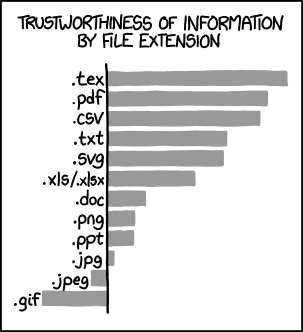
\includegraphics[scale=0.4]{Graphiques/file_extensions}
					\caption{\href{http://xkcd.com/}{\copyright\ xkcd}}
				\label{Graphiques_extensions}
			\end{figure}


  		\subsection{Pour ins�rer une figure...}
			
\code
\begin{figure}
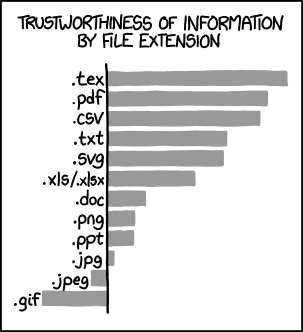
\includegraphics[scale=1]{Graphiques/file_extensions}
\caption{\href{http://xkcd.com/}{\copyright\ xkcd}}
\label{Graphiques_extensions}
\end{figure}
\end{Verbatim}


			
			L'environnement \textit{figure} correspond � un des mots-clefs qui d�finisse un flottant.
			
\code
\begin{figure}
\end{Verbatim}

			Puis la commande suivante indique le nom et le chemin du fichier image. 
			
\code			
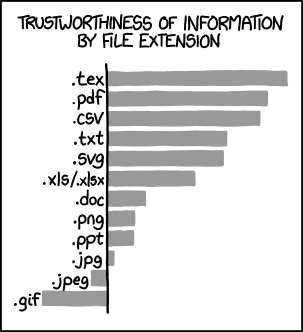
\includegraphics[scale=0.4]{Graphiques/file_extensions}
\end{Verbatim}

		A noter �galement l'argument \emph{scale} qui permet de d�terminer en proportion la taille de l'image par rapport � l'original.



			La commande suivante permet d'indiquer une l�gende,
			
\code			
\caption{\href{http://xkcd.com/}{\copyright\ xkcd}}
\end{Verbatim}

			Puis un label est d�fini pour y faire r�f�rence. 
			
\code			
\label{Graphiques_extensions}
\end{figure}
\end{Verbatim}



			Enfin on ferme la balise du flottant~:			
			
\code			
\end{figure}
\end{Verbatim}


\section{Exemple, ins�rer un tableau}

  		\subsection{Pour ins�rer un tableau...}
  		
  		Ins�rer un tableau est similaire sur le principe � une image. 
  		
  		Les tableaux utilisent le mot-clef \emph{table}. 
  		
			\begin{center}
				\begin{table}[h!]
					\begin{tabular}{lcccccc}
						\hline
						 & CR & HN & B1 & B2 & C1 & C2 \\ 
						\hline
						Indulgent & 0 & 19 & 39 & 32 & 7 & 1 \\ 
						\hline
					\end{tabular}
					\caption[position=bottom]{R�partition des niveaux}
					\label{Tableau:Niveaux}
				\end{table}  		
			\end{center}


  		
\tinycode			
\begin{center}
	\begin{table}[h!]
		% D�but Tableau
		\begin{tabular}{lcccccc}
			\hline
			 & CR & HN & B1 & B2 & C1 & C2 \\ 
			\hline
			Indulgent & 0 & 19 & 39 & 32 & 7 & 1 \\ 
			\hline
		\end{tabular}
		% Fin Tableau
		\caption[position=bottom]{R�partition des niveaux}
		\label{Tableau:Niveaux}
	\end{table}  		
\end{center}
\end{Verbatim}


\section{Notion de bloc}

  		\subsection{Tout est bloc...}
  		
  		La base de la mise en page dans \latex sont des blocs.
  		\vspace{0.3cm}
  		Une lettre, un mot, un paragraphe, un flottant, ... 
  		\vspace{0.3cm}
  		Tout est organis� sous la forme de blocs.
  		\vspace{0.3cm}
  		Donc ce type de choses est possible~:\\
  		\vspace{0.3cm}
			\LaTeX~\raisebox{-0.5em}{f}onctionne \raisebox{-0.5em}{par} bo�te \raisebox{0.5em}{m�me} pour un mot, une lettre...
	  		  		

  		
  		La commande \emph{raisebox} permet d'illustrer ce principe~: elle d�cale le centre de la bo�te d'une certaine hauteur.
			\vspace{0.3cm}
			
\LaTeX~\raisebox{-0.5em}{f}onctionne \raisebox{-0.5em}{par} bo�te \raisebox{0.5em}{m�me} pour un mot, une lettre...
			  		
\tinycode
\LaTeX~\raisebox{-0.5em}{f}onctionne \raisebox{-0.5em}{par} bo�te %
\raisebox{0.5em}{m�me} pour un mot, une lettre...
\end{Verbatim}


		
		
		La commande \emph{fbox} permet d'encadrer le texte et de visualiser ces blocs...
		\vspace{0.3cm}
		
\LaTeX~\fbox{f}onctionne \fbox{par} bo�te 
\fbox{m�me} pour un mot, une lettre...

\tinycode
\LaTeX~\fbox{-0.5em}{f}onctionne \fbox{par} bo�te 
\fbox{m�me} pour un mot, une lettre...
\end{Verbatim}
					  		  		
  	
		
		Par cons�quent, des commandes permettant de transformer la position ou l'orientation vont fr�quemment marcher pour un mot, un paragraphe, un flottant...
		\vspace{0.3cm}
		
		\LaTeX fontionne \raisebox{-0.5ex}{par} bloc \raisebox{-0.45\height}{\rotatebox{45}{ce qui est}} pratique.
		
\tinycode
\LaTeX fontionne \raisebox{-0.5ex}{par} bloc %
\raisebox{-0.45\height}{\rotatebox{45}{ce qui est}} pratique.
\end{Verbatim}
			  		  		
  	
		
		\begin{center}
		\scalebox{0.6}{\raisebox{-0.5\height}{\rotatebox{45}{\begin{minipage}{0.8\linewidth}\lipsum[1]\end{minipage}}}}
		\end{center}

  	
  	

			Il y a une petite subtilit�... On doit d�finir quelque part la largeur du paragraphe d'o� l'utilisation de \emph{minipage}
			
\tinycode
\scalebox{0.6}{
	\raisebox{-0.5\height}{
		\rotatebox{45}{
			\begin{minipage}{0.8\linewidth}
				\lipsum[1]
			\end{minipage}
		}
	}
}
\end{Verbatim}
		
			  		  		

  		
% Table generated by Excel2LaTeX from sheet 'USHealth'
\begin{table}[h!]
  \centering
	\rotatebox{45}{\scalebox{0.3}{
    \begin{tabular}{rrrrrrrr}
    \addlinespace
    \toprule
    {\bf State:} & {\bf Smokers} & {\bf Smoke everyday} & {\bf PhysicalActivity} & {\bf HighPhysicalActivity} & {\bf LimitedActivities} & {\bf Obese} & {\bf Stroke} \\
    \midrule
    {\bf Alabama} & 22,5  & 16,5  & 21,1  & 41,1  & 23,5  & 31,6  & 3,9 \\
    {\bf Alaska} & 20,6  & 14,7  & 40,1  & 60,7  & 21,4  & 25,4  & 1,9 \\
    {\bf Arizona} & 16,1  & 11    & 30,1  & 50,5  & 18,6  & 25,9  & 2,6 \\
    {\bf Arkansas} & 21,5  & 15,5  & 25,3  & 47,3  & 22,8  & 31,5  & 3,6 \\
    {\bf California} & 12,9  & 8,1   & 32,9  & 51,3  & 17,2  & 25,5  & 2,3 \\
    {\bf Colorado} & 17,1  & 12,1  & 34,6  & 57,1  & 18    & 19    & 1,4 \\
    {\bf Connecticut} & 15,4  & 10,7  & 32    & 53,9  & 16,1  & 21    & 1,6 \\
    {\bf Delaware} & 18,3  & 13,3  & 29,3  & 51    & 18,3  & 27,6  & 2,7 \\
    {\bf District of Columbia} & 15,3  & 9,1   & 34,1  & 54,5  & 16,1  & 20,1  & 2,6 \\
    {\bf Florida} & 17,1  & 12,8  & 25,6  & 46,2  & 20,9  & 26,5  & 3 \\
    {\bf Georgia} & 17,7  & 12,6  & 27,5  & 45,7  & 16    & 27,7  & 2,3 \\
    {\bf Guam} & 24,1  & 18,9  & 26,5  & 47,4  & 11    & 26,8  & 2,1 \\
    {\bf Hawaii} & 15,4  & 10,4  & 34,5  & 53,2  & 14,9  & 22,9  & 2,5 \\
    {\bf Idaho} & 16,3  & 12,3  & 36    & 57,5  & 20,1  & 25,1  & 2,5 \\
    {\bf Illinois} & 18,6  & 12    & 31,8  & 51,8  & 16    & 27,4  & 2,4 \\
    {\bf Indiana} & 23,1  & 17,1  & 28,2  & 48    & 20    & 30    & 2,6 \\
    {\bf Iowa} & 17,2  & 13,4  & 26,9  & 49,7  & 16,4  & 28,5  & 2,4 \\
    {\bf Kansas} & 17,8  & 13,2  & 27,5  & 48,5  & 18,9  & 28,8  & 2,6 \\
    {\bf Kentucky} & 25,6  & 20,6  & 23,6  & 45,7  & 24,8  & 32,4  & 3,7 \\
    \bottomrule
    \end{tabular}
		}}
  \label{tab:addlabel}
\end{table}  	
  	

  		

\tinycode
% Table generated by Excel2LaTeX from sheet 'USHealth'
\begin{table}[h!]
  \centering
	\rotatebox{45}{
		\scalebox{0.3}{
			% Tableau
			\begin{tabular}{rrrrrrrr}
				\addlinespace
				\toprule
				{\bf State:} & {\bf Smokers} & {\bf Smoke everyday} ... 
				\midrule
				{\bf Alabama} & 22,5  & 16,5  & 21,1  & 41,1  & 23,5  ...\\
				...
				{\bf Kentucky} & 25,6  & 20,6  & 23,6  & 45,7  & 24,8  ... \\
				\bottomrule
			\end{tabular}
			%Fin Tableau
		}
	}
  \label{tab:addlabel}
\end{table}
\end{Verbatim}  		
  
  		  	  	 



\section{Un tableau pas � pas}

  		\subsection{Un tableau pas � pas}
  		
  		Voici un exemple concis de tableau...
  		
\begin{center}
\begin{table}[h!]
	\begin{tabular}{lcccccc}
		\hline
		 & CR & HN & B1 & B2 & C1 & C2 \\ 
		\hline
		Indulgent & 0 & 19 & 39 & 32 & 7 & 1 \\ 
		\hline
	\end{tabular}
	\caption[position=bottom]{R�partition des niveaux}
	\label{Tableaux_Niveaux}
\end{table}  		
\end{center}
  		
		
  		
  		Voici un exemple concis de tableau...
  		
\begin{Verbatim}[frame=single,label=Code]
\begin{table}[h!]
	\begin{tabular}{lcccccc}
		\hline
		 & CR & HN & B1 & B2 & C1 & C2 \\ 
		\hline
		Indulgent & 0 & 19 & 39 & 32 & 7 ...
		\hline
	\end{tabular}
	\caption[position=bottom]{R�partition des ...
	\label{Tableau:Niveaux}
\end{table}  		
\end{Verbatim}
  		

	
			On initialise le flottant, un tableau, avec l'environnement \textit{table}.
  		
  		\begin{Verbatim}[frame=single,label=Code]
\begin{table}[h!]
			\end{Verbatim}

			L'argument optionnel indique que le compilateur doit si possible le placer \og~ici~\fg, ie. � cet endroit du document (par rapport au texte environnant).

	
	
			Si \textit{figure} d�finit le flottant, le tableau est r�ellement d�fini par l'environnement \emph{tabular}.
			\begin{Verbatim}[frame=single,label=Code]
\begin{tabular}{lcccccc}
			\end{Verbatim}
			
			Le deuxi�me argument, obligatoire, indique � la fois la justification du texte et le nombre de colonnes.
			
			Dans ce cas, il y a six colonnes~: le texte de la premi�re colonne est justifi� � gauche et celui des 6 suivantes est centr�.

			Pour la position, les possibilit�s sont~: \textit{c} pour centr�, \textit{l} pour gauche (left) et \textit{r} pour droite.



			Si on veut ajouter des lignes de s�paration verticale sur toute la hauteur du tableau, il suffit d'ajouter des \textbar~entre chaque indication de position. 
			\begin{Verbatim}[frame=single,label=Code]
\begin{tabular}{|l|c|ccccc|}
			\end{Verbatim}

			donnerait...


  		
\begin{center}
\begin{table}[h!]
	\begin{tabular}{|l|c|ccccc|}
		\hline
		 & CR & HN & B1 & B2 & C1 & C2 \\ 
		\hline
		Indulgent & 0 & 19 & 39 & 32 & 7 & 1 \\ 
		\hline
	\end{tabular}
	\caption[position=bottom]{R�partition des niveaux}
	\label{Tableau:Niveaux}
\end{table}  		
\end{center}
  		
		
	
			Pour faire une ligne horizontale... Il faut placer entre deux lignes~:
			\vspace{0.5cm}
			\begin{Verbatim}[frame=single,label=Code]
  \hline
			\end{Verbatim}

			Pour faire une double ligne horizontale... Il faut placer entre deux lignes~:
			\vspace{0.5cm}
			\begin{Verbatim}[frame=single,label=Code]
  \hline \hline
			\end{Verbatim}
			
			et ainsi de suite\dots
			

			
			La syntaxe pour rentrer les donn�es utilise deux �lements~: le \&~comme s�paration des colonnes et le \textbackslash \textbackslash~permet de clore la ligne et retourner � la ligne suivante.
			\vspace{0.3cm}
			\begin{Verbatim}[frame=single,label=Code]
 & CR & HN & B1 & B2 & C1 & C2\\ 			
			\end{Verbatim}
			
			A l'exception de la fin de la ligne, un tableau sous \latex a une structure proche de celle d'un fichier CSV.

	

			Ne reste plus qu'� fermer le tableau
			\vspace{0.5cm}
			\begin{Verbatim}[frame=single,label=Code]
\end{tabular}
			\end{Verbatim}
						
					
  		\subsection{Le tableau pas � pas}
		
			Une fois l'environnement \textit{tabular} ferm�, nous nous trouvons toujours � l'int�rieur du flottant (\textit{table}).
			
			Cela permet d'ajouter une l�gende situ�e en dessous du tableau...
			\vspace{0.3cm}
			\begin{Verbatim}[frame=single,label=Code]
\caption[position=bottom]{R�partition des niveaux}
			\end{Verbatim}

			Ici on pr�cise la position de l�gende avec l'argument \emph{position}. Mais le plus simple est de mettre \emph{caption} au-dessus du groupe \emph{tabular} pour avoir la l�gende en haut et inversement.
			

			
			Et un petit nom pour lui faire r�f�rence dans le texte...

		\begin{Verbatim}[frame=single,label=Code]
\label{Tableau_Niveaux}
		\end{Verbatim}
		
		Pour y faire r�f�rence ensuite, il suffira d'utiliser le code suivant~:
		\vspace{0.3cm}
		\begin{Verbatim}[frame=single,label=Code]		
\ref{Tableaux_Niveaux}
		\end{Verbatim}


Exemple : 
La tableau \ref{Tableaux_Niveaux} repr�sente la r�partition des niveaux.
			\vspace{0.3cm}
		\begin{Verbatim}[frame=single,label=Code]		
La tableau \ref{Tableaux_Niveaux} repr�sente 
la r�partition des niveaux.
		\end{Verbatim}

				

			Enfin il faut fermer l'environnement ouvert au d�but~:

		\code			
\end{table}  		
  	\end{Verbatim}
  		
		
\section{La mise en page des tableaux}

  		\subsection{Les bordures}

			Comme vu pr�cedemment, les bordures pour une ligne horizontale sont g�n�r�es par la commande \emph{\textbackslash hline}.
			
			Pour les bordures verticales sont d�finies dans l'argument de la commande \emph{tabular}.
			
			Si on veut ajouter des bordures horizontales entre quelques cellules seulement on utilise la commande \emph{\textbar cline} qui ajoute entre les colonnes pr�cis�es une bordure en dessous :

\begin{center}
\begin{tabular}{cccc}
\hline
Colonne 1 & Colonne 2 & Colonne 3 & Colonne 4\\
\hline
1 & 2 & 3 & 4\\
\cline{3-4}
1 & 2 & 3 & 4\\
\cline{2-4}
1 & 2 & 3 & 4\\
\hline
\end{tabular}			
\end{center}



\code
\begin{tabular}{cccc}
\hline
Colonne 1 & Colonne 2 & Colonne 3 & Colonne 4\\
\hline
1 & 2 & 3 & 4\\
\cline{3-4}
1 & 2 & 3 & 4\\
\cline{2-4}
1 & 2 & 3 & 4\\
\hline
\end{tabular}			
\end{Verbatim}



			Pour les lignes verticales sur certaines lignes, il y a la possibilit� d'utiliser \emph{\textbackslash vline}.
			
\begin{center}
\begin{tabular}{cccc}
\hline
Colonne 1 & Colonne 2 & Colonne 3 & Colonne 4\\
\hline
\vline  1  \vline & 2 & 3 & 4\\
 1  \vline & \vline 2  \vline & 3 & 4\\
1 & 2 & 3 & \vline 4  \vline \\
\hline
\end{tabular}			
\end{center}

	Mais le r�sultat n'est pas tr�s satisfaisant. 

		
		
\code
\begin{tabular}{cccc}
	\hline
	Colonne 1 & Colonne 2 & Colonne 3 & Colonne 4\\
	\hline
	\vline 1 \vline & 2 & 3 & 4\\
	1 \vline & \vline 2 \vline & 3 & 4\\
	1 & 2 & 3 & \vline 4 \vline \\
	\hline
\end{tabular}			
\end{Verbatim}

		La bordure est plac�e autour du texte et non aux extr�mit�s de la cellule.  

		
			
			Une premi�re solution pour contourner le probl�me consiste � dessiner la bordure avant ou apr�s la commande \emph{\textbackslash hfill}.
		\vspace{0.4cm}
		
\code
\begin{tabular}{cccc}
	\hline
	Colonne 1 & Colonne 2 & Colonne 3 & Colonne 4\\
	\hline
	\vline \hfill 1 \hfill \vline & 2 & 3 & 4\\
	\hfill 1 \hfill \vline & \vline \hfill 2 \hfill \vline & 3 & 4\\
	1 & 2 & 3 & \vline \hfill 4 \hfill \vline \\
	\hline
\end{tabular}			
\end{Verbatim}
		
		Mais le r�sultat n'est pas parfait. Y'a un tout petit d�calage parfois (2\up{�me} et 3\up{�me} ligne).

		
			
\begin{center}
\begin{tabular}{cccc}
	\hline
	Colonne 1 & Colonne 2 & Colonne 3 & Colonne 4\\
	\hline
	\vline \hfill 1 \hfill \vline & 2 & 3 & 4\\
	\hfill 1 \hfill \vline & \vline \hfill 2 \hfill \vline & 3 & 4\\
	1 & 2 & 3 & \vline \hfill 4 \hfill \vline \\
	\hline
\end{tabular}			
\end{center}
		
		Pour obtenir un r�sultat parfait, il faut utiliser le package \emph{multicolumn} d�crit � la section suivante.

		

			
\begin{center}
\begin{tabular}{cccc}
	\hline
	Colonne 1 & Colonne 2 & Colonne 3 & Colonne 4\\
	\hline
	\multicolumn{1}{c|}{1} & 2 & 3 & 4\\
	\multicolumn{1}{c|}{1} & \multicolumn{1}{c|}{2} & 3 & 4\\
	1 & 2 & 3 & \multicolumn{1}{c|}{4} \\
	\hline
\end{tabular}			
\end{center}
		
		
			
\code
\begin{tabular}{cccc}
	\hline
	Colonne 1 & Colonne 2 & Colonne 3 & Colonne 4\\
	\hline
	\multicolumn{1}{c|}{1} & 2 & 3 & 4\\
	\multicolumn{1}{c|}{1} & \multicolumn{1}{c|}{2}...
	1 & 2 & 3 & \multicolumn{1}{c|}{4} \\
	\hline
\end{tabular}			
\end{Verbatim}

		Cela marche parfaitement car dans ce cas \latex, via la commande \emph{multicolumn}, est oblig� de calculer pr�cisement la taille de la cellule.
		
				
\section{La fusion de cellules}

  		\subsection{multicolumn}

			Justement, pour fusionner des colonnes on peut utiliser la commande~:	
			\vspace{0.4cm}
					
			\code
\multicolumn{ nombre }{ description }{ contenu }
			\end{Verbatim}

			\emph{nombre} indique le nombre de colonnes concern�es par la fusion.

			Le contenu de \emph{description} est identique � l'argument de \emph{tabular}, ie~:
			
			\code
\multicolumn{2}{|c|}{texte}
			\end{Verbatim}



\begin{tabular}{|l|l|l|l|}
\hline
Colonne 1 & Colonne 2 & Colonne 3 & Colonne 4\\
\hline
\multicolumn{2}{c}{Fusion} & 1 & 2\\
\hline
3 & \multicolumn{3}{c}{Fusion}\\
\hline
4 & 5 & 6 & 7 \\
\hline
\end{tabular}			



		\code
\begin{tabular}{|l|l|l|l|}
\hline
Colonne 1 & Colonne 2 & Colonne 3 & Colonne 4\\
\hline
\multicolumn{2}{c}{Fusion} & 1 & 2\\
\hline
3 & \multicolumn{3}{c}{Fusion}\\
\hline
4 & 5 & 6 & 7 \\
\hline
\end{tabular}			
		\end{Verbatim}
	


		Les lignes verticales ont disparues~! Pour les retrouver, exactement comme dans la syntaxe de \emph{tabular}, on les ajoute autour de la cellule.
		
\begin{tabular}{|l|l|l|l|}
\hline
Colonne 1 & Colonne 2 & Colonne 3 & Colonne 4\\
\hline
\multicolumn{2}{|c|}{Fusion} & 1 & 2\\
\hline
3 & \multicolumn{3}{c|}{Fusion}\\
\hline
4 & 5 & 6 & 7 \\
\hline
\end{tabular}		
	
		

\code
\begin{tabular}{|l|l|l|l|}
	\hline
	Colonne 1 & Colonne 2 & Colonne 3 & Colonne 4\\
	\hline
	\multicolumn{2}{|c|}{Fusion} & 1 & 2\\
	\hline
	3 & \multicolumn{3}{c|}{Fusion}\\
	\hline
	4 & 5 & 6 & 7 \\
	\hline
\end{tabular}		
\end{Verbatim}
	

  		\subsection{multirow}

			Le paquet \emph{multirow} permet de fusionner des lignes.
			\vspace{0.3cm}
			\code
\multirow{nombreLignes}{largeur}{contenu}
			\end{Verbatim}

			La largeur peut �tre tout simplement \emph{*} pour une largeur automatique. Comme pour le \emph{multicolumn}, il faut ajuster les bordures...



			\begin{tabular}{|l|l|l|l|}\hline
				Le texte \no1 &Le texte \no1 & ligne1 & ligne 1\\ 
				\hline
				\multirow{3}{*}{texte2} & \multirow{3}{3cm}{texte2} & ligne2 & \multirow{2}{*}{texte3} \\
				\cline{3-3}
				& & ligne3 & \\ 
				\cline{3-4}            
				& & ligne4 & Fin \\\hline
			\end{tabular}



\begin{Verbatim}[fontsize=\tiny,frame=single,label=Code]
\begin{tabular}{|l|l|l|l|}
	\hline
	Le texte & Le texte & ligne1 & ligne 1\\
	\hline
	\multirow{3}{*}{texte2} & \multirow{3}{*}{texte2} %
	   & ligne2 & \multirow{2}{*}{texte3}\\
	\cline{3-3}            
	&   & ligne3 & \\ 
	\cline{3-4}            
	&   & ligne4 & Fin\\
	\hline
\end{tabular}
\end{Verbatim}

		
  	\subsection{Rotation du texte}
  								
    La rotation d'un objet peut �tre r�alis� par exemple avec la commande \emph{sideways} qui provient du paquet \emph{rotating}...
\vspace{0.3cm}

\begin{Verbatim}[fontsize=\tiny,frame=single,label=Code]
...
\begin{sideways}Population PISA\end{sideways} & Moyenne & 250 \\
\hline
\addlinespace
\begin{sideways}1\ere \end{sideways} & Moyenne & 260 \\
...
\end{Verbatim}


  								
\begin{table}[htbp]
\begin{center}
\begin{tabular}{cc|c}
\begin{sideways}Population PISA\end{sideways} & Moyenne & 250 \\
\hline
\addlinespace
\begin{sideways}1ere\end{sideways} & Moyenne & 260 \\
\end{tabular}
\end{center}
\end{table}


\section{Excel2LaTeX}

  		\subsection{Excel to \LaTeX}

			Il faut conna�tre la syntaxe mais vous avez la possibilit� de transformer un tableau Excel en tableau \latex.
			
			La macro \href{https://www.ctan.org/pkg/excel2latex}{Exce2\latex} permet en un clic d'exporter un tableau Excel avec sa mise en forme sous \LaTeX.
			
			Un clic permet de g�n�rer le code qui peut �tre stock� dans un fichier ou bien copi�/coll� dans un �diteur de texte.

			La macro est compatible avec Microsoft Office 2010, 2013, \dots



			Il faut inclure le paquet \emph{booktabs} dans le pr�ambule du document car la macro utilise ce paquet pour la mise en forme. 
			
			La macro ne permet pas de rendre la totalit� de la mise en page mais cela permet souvent de cr�er le tableau de base que l'on am�liore par la suite.
			
			Si on veut modifier le tableau \emph{a posteriori} ou utiliser par \emph{longtable}, dans ce cas il ne faut pas utiliser la syntaxe de \emph{booktabs}. La macro permet de le faire, il suffit de cocher la case � cocher correspondante.
						


		\begin{center}
			\scalebox{0.3}{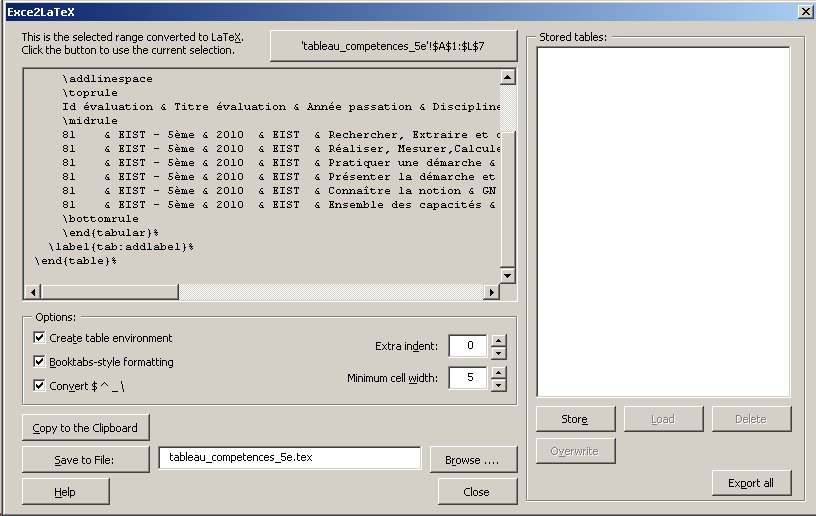
\includegraphics{Graphiques/Excel2LaTeX.jpg}}
		\end{center}
						
		
				

			Une sortie de la macro Excel~:

\begin{table}[htbp]
  \centering
\scalebox{0.7}{
    \begin{tabular}{rrrr}
    \addlinespace
    \toprule
    {\bf State:} & {\bf Smokers} & {\bf Smoke everyday} & {\bf PhysicalActivity}\\
    \midrule
    {\bf Alabama} & 22,5  & 16,5  & 21,1  \\
    {\bf Alaska} & 20,6  & 14,7  & 40,1   \\
    {\bf Arizona} & 16,1  & 11    & 30,1   \\
    {\bf Arkansas} & 21,5  & 15,5  & 25,3  \\
    {\bf California} & 12,9  & 8,1   & 32,9   \\
    {\bf Colorado} & 17,1  & 12,1  & 34,6   \\
    {\bf Connecticut} & 15,4  & 10,7  & 32  \\
    {\bf Delaware} & 18,3  & 13,3  & 29,3  \\
    {\bf District of Columbia} & 15,3  & 9,1  \\
    {\bf Florida} & 17,1  & 12,8  & 25,6  \\
    \bottomrule
    \end{tabular}
}
  \label{tab:addlabel}
\end{table}

		
\section{Couleurs}

  		\subsection{Colorer les lignes}
                
Le paquet xcolor appel� dans le pr�ambule permet de colorer en alternance les lignes. Inconv�nient, il rentre en conflit avec quelques paquets.
                
\code
\usepackage[table]{xcolor}
\end{Verbatim}



La coloration est r�alis�e par cette commande~:
\vspace{0.5cm}

\code 
\rowcolors{2}{myblue4}{myblue5}
<Tableau>
\rowcolors{2}{white}{white}
\end{Verbatim}

La deuxi�me ligne, apr�s le tableau, permet de r�initialiser les param�tres par d�faut pour pr�server les tableaux (et figures) suivants.



  		
Sinon on peux utiliser le package \emph{colortbl}

\begin{table}[h!]
\begin{center}
\begin{tabular}{l|cccccc}
  \hline
 \rowcolor{blue}& CR & HN & B1 & B2 & C1 & C2 \\ 
  \hline
  Indulgent & 0.00 & 19.40 & 39.30 & 32.70 & 7.40 & 1.20 \\ 
  S�v�re (Consignes) & 46.60 & 6.40 & 18.90 & 21.60 & 5.50 & 0.90 \\ 
  Indulgent (Consignes) & 46.60 & 4.70 & 18.50 & 22.80 & 6.30 & 1.10 \\ 
   \hline
\end{tabular}
\caption[position=top]{R�partition des niveaux}
\label{Tableau:Niveaux}
\end{center}
\end{table} 



La commande est tout simplement~:
\vspace{0.5cm}

\code
\hline
\rowcolor{blue}& CR & HN & B1 & B2 & C1 & C2 \\ 
\hline
\end{Verbatim}



  		\subsection{Colorer des colonnes}

			C'est possible avec le m�me paquet m�me en utilisant la commande \emph{multicolumn}.
			
			La couleur de la colonne est d�clar�e directement dans les arguments de \emph{tabular}~:
			
\code
\begin{tabular}{l l >{\columncolor{green}} l}
   1 & 2 & 3 \\
   a & b & c
\end{tabular}
\end{Verbatim}


	
\begin{table}[h!]
\begin{tabular}{l l >{\columncolor{green}} l}
   1 & 2 & 3 \\
   a & b & c
\end{tabular}
\end{table}


\section{Gestion des grands tableaux}

  		\subsection{Tableau trop large}
  		
Dans ce cas il est souvent appr�ciable de faire pivoter le tableau ou la page.

C'est possible avec le paquet \emph{rotating} d�j� utilis�~:
                
\begin{description}
\item [sideways] pour tourner toute la page de 90�.
\item [sidewaystable] pour tourner le tableau de 90�.
\item [turn, rotate] pour tourner le contenu de x�.
\end{description}


  		
			Par exemple...

\begin{center}               
\begin{table}[h!]
\begin{sideways}\scalebox{0.4}{
\begin{tabular}{l|cccccc}
  \hline
 	\rowcolor{blue}& CR & HN & B1 & B2 & C1 & C2 \\ 
  \hline
  Indulgent & 0.00 & 19.40 & 39.30 & 32.70 & 7.40 & 1.20 \\ 
  S�v�re (Consignes) & 46.60 & 6.40 & 18.90 & 21.60 & 5.50 & 0.90 \\ 
  Indulgent (Consignes) & 46.60 & 4.70 & 18.50 & 22.80 & 6.30 & 1.10 \\ 
  \hline
\end{tabular}}
\end{sideways}
\caption[position=top]{R�partition des niveaux}
\label{Tableau:Niveaux}
\end{table} 
\end{center}



 			Comme dans l'exemple pr�c�dent, la rotation est la r�duction de la taille est possible car un tableau repr�sente un bloc. De ce fait, on peux utiliser toutes les commandes aff�rentes � un bloc.

			Le code du tableau pr�c�dent est finalement assez simple si on pense � fait que (presque) tout �lement de \latex est un bloc.



\begin{Verbatim}[fontsize=\tiny,frame=single,label=Code]
\begin{table}[h!]
	\begin{sideways}
		\scalebox{0.4}{
			\begin{tabular}{l|cccccc}
				\hline
				\rowcolor{blue}& CR & HN & B1 & B2 & C1 & C2 \\ 
				\hline
				Indulgent & 0.00 & 19.40 & 39.30 & 32.70 & 7.40 & 1.20 \\ 
				Indulgent (Consignes) & 46.60 & 4.70 & 18.50 & 22.80 & 6.30 & 1.10 \\ 
				\hline
			\end{tabular}
		}
	\end{sideways}
	\caption[position=top]{R�partition des niveaux}
	\label{Tableau:Niveaux}
\end{table} 
\end{Verbatim}



% Table generated by Excel2LaTeX from sheet 'USHealth'
\begin{table}[h!]
  \centering
	\scalebox{0.45}{
    \begin{tabular}{rrrrrrrr}
    \addlinespace
    \toprule
    {\bf State:} & {\bf Smokers} & {\bf Smoke everyday} & {\bf PhysicalActivity} & {\bf HighPhysicalActivity} & {\bf LimitedActivities} & {\bf Obese} & {\bf Stroke} \\
    \midrule
    {\bf Alabama} & 22,5  & 16,5  & 21,1  & 41,1  & 23,5  & 31,6  & 3,9 \\
    {\bf Alaska} & 20,6  & 14,7  & 40,1  & 60,7  & 21,4  & 25,4  & 1,9 \\
    {\bf Arizona} & 16,1  & 11    & 30,1  & 50,5  & 18,6  & 25,9  & 2,6 \\
    {\bf Arkansas} & 21,5  & 15,5  & 25,3  & 47,3  & 22,8  & 31,5  & 3,6 \\
    {\bf California} & 12,9  & 8,1   & 32,9  & 51,3  & 17,2  & 25,5  & 2,3 \\
    {\bf Colorado} & 17,1  & 12,1  & 34,6  & 57,1  & 18    & 19    & 1,4 \\
    {\bf Connecticut} & 15,4  & 10,7  & 32    & 53,9  & 16,1  & 21    & 1,6 \\
    {\bf Delaware} & 18,3  & 13,3  & 29,3  & 51    & 18,3  & 27,6  & 2,7 \\
    {\bf District of Columbia} & 15,3  & 9,1   & 34,1  & 54,5  & 16,1  & 20,1  & 2,6 \\
    {\bf Florida} & 17,1  & 12,8  & 25,6  & 46,2  & 20,9  & 26,5  & 3 \\
    {\bf Georgia} & 17,7  & 12,6  & 27,5  & 45,7  & 16    & 27,7  & 2,3 \\
    {\bf Guam} & 24,1  & 18,9  & 26,5  & 47,4  & 11    & 26,8  & 2,1 \\
    {\bf Hawaii} & 15,4  & 10,4  & 34,5  & 53,2  & 14,9  & 22,9  & 2,5 \\
    {\bf Idaho} & 16,3  & 12,3  & 36    & 57,5  & 20,1  & 25,1  & 2,5 \\
    {\bf Illinois} & 18,6  & 12    & 31,8  & 51,8  & 16    & 27,4  & 2,4 \\
    {\bf Indiana} & 23,1  & 17,1  & 28,2  & 48    & 20    & 30    & 2,6 \\
    {\bf Iowa} & 17,2  & 13,4  & 26,9  & 49,7  & 16,4  & 28,5  & 2,4 \\
    {\bf Kansas} & 17,8  & 13,2  & 27,5  & 48,5  & 18,9  & 28,8  & 2,6 \\
    {\bf Kentucky} & 25,6  & 20,6  & 23,6  & 45,7  & 24,8  & 32,4  & 3,7 \\
    \bottomrule
    \end{tabular}
		}
  \label{tab:addlabel}
\end{table}


\begin{Verbatim}[fontsize=\tiny,frame=single,label=Code]
% Table generated by Excel2LaTeX from sheet 'USHealth'
\begin{table}[h!]
  \centering
		\scalebox{0.45}{
			\begin{tabular}{rrrrrrrr}
				\addlinespace
				\toprule
				{\bf State:} & {\bf Smokers} & {\bf Smoke everyday} ... 
				\midrule
				{\bf Alabama} & 22,5  & 16,5  & 21,1  & 41,1  & 23,5  & 31,6  & 3,9 \\
				...
				{\bf Kentucky} & 25,6  & 20,6  & 23,6  & 45,7  & 24,8  & 32,4  & 3,7 \\
				\bottomrule
			\end{tabular}
		}
  \label{tab:addlabel}
\end{table}
\end{Verbatim}



  		\subsection{Tableau trop large en PDF}

Le paquet \emph{lscape} permet sp�cifiquement de tourner la page en mode paysage ce qui est support� par le format PDF. Les commandes ci-dessous suffisent.

\code
\usepackage{lscape}
...
\begin{landscape}
Some text
\end{landscape}
\end{Verbatim}


  		\subsection{Tableau trop long}

Quant au paquet \emph{longtable}, il permet de r�aliser un tableau s'�talant sur plusieurs pages.

Il permet notamment un contr�le fin des ent�tes et pieds de page du tableau.



\tinycode
\begin{longtable}{ | p{0.2\linewidth} | p{0.2\linewidth} | p{0.2\linewidth} | }
	Premiere colonne & Deuxieme & Troisieme 
	\endfirsthead
	
	Premiere & Deuxieme & Troisieme \\
	\multicolumn{3}{|p{0.6666\linewidth}|}{Suite ... } \\
	\endhead

	\multicolumn{3}{|p{0.6666\linewidth}|}{Suite page suivante}\\ 
	\hline 
	\endfoot 
	
	\hline
	\multicolumn{3}{|p{0.6666\linewidth}|}{C'est fini} \\
	\endlastfoot 
	
	\hline
	1   &     1  &        1  \\
	...
\end{longtable}
\end{Verbatim}


%
%\begin{longtable}
%   {|p{0.2\linewidth}|p{0.2\linewidth}|p{0.2\linewidth}|}
%   \hline
%   Premiere colonne & Deuxieme & Troisieme \endfirsthead
%   \hline
%   Premiere & Deuxieme & Troisieme \\
%   \multicolumn{3}{|p{0.6666\linewidth}|}{Suite ... } \\
%   \endhead
%   \hline
%   \multicolumn{3}{|p{0.6666\linewidth}|}{Suite page suivante}
%   \\ \hline \endfoot \hline
%   \multicolumn{3}{|p{0.6666\linewidth}|}{C'est fini} \\
%   \hline
%   \endlastfoot \hline
%   1   &     1  &        1  \\
%   2   &     4  &       16  \\
%   3   &     9  &       81  \\
%   1   &     1  &        1  \\
%   2   &     4  &       16  \\
%   3   &     9  &       81  \\
%   1   &     1  &        1  \\
%   2   &     4  &       16  \\
%   3   &     9  &       81  \\
%   1   &     1  &        1  \\
%   2   &     4  &       16  \\
%   3   &     9  &       81  \\
%\end{longtable}
%
%
%
%


% Rajouter une partie sur les clauses de taille dans l'argument des tabular. Dans Couleurs et...



		



\section{Les formats d'image}		

  		\subsection{Les formats de fichier reconnus}
  		
  		Tous les formats d'images ne sont pas support�s par LaTeX...
  		
  		Si on compile vers un fichier de format~:
  		\begin{description}
  			\item[Postscript (.ps)] on peut ins�rer que des images au format Postscript
  			\item[PDF (.pdf)] on peut ins�rer des images au format jpeg, pdf, png, ...
  		\end{description}
  		



			Les formats d'image sont tourn�s vers les standards \emph{ouverts}.
			
			Par cons�quent, il n'existe pas de moyen d'importer des images de \emph{wmf} par exemple.
			
			Dans ce cas on tentera de convertir le fichier en format de fichier reconnu. 
			
			A cet �gard, un outil tr�s puissant de conversion d'images est \href{http://www.imagemagick.org}{ImageMagick}. 
			
			Une interface graphique existe mais son potentiel se r�v�le surtout en ligne en commande.
  		


			Il existe des outils permettant de faire des images directement � l'int�rieur de \latex.
			
			\begin{itemize}
				\item des sch�mas
				\item des dessins et notamment des dessins g�om�triques
				\item des graphiques issus de donn�es statistiques
				\item ...
			\end{itemize}
			
			Ces outils sont des langages � utiliser � l'int�rieur de \latex. 
			


			Ne seront cit�s ici que les trois plus connus et qui permettent tous les trois d'accomplir les t�ches pr�c�demment cit�es~:
			
			\begin{description}
				\item[Metapost] c'est un langage cr�� par D. \textsc{Knuth}, le cr�ateur de \tex. Extr�mement puissant mais il demande un certain temps d'apprentissage.
				\item[PSTricks] ce language permet de cr�er des images Postscript. Il est beaucoup plus accessible mais a certaines limitations.
				\item[TikZ/PGF] Probablement le plus accessible et le plus pratique mais certaines limitations comme l'absence de graphiques en 3 dimensions par exemple.
			\end{description}
			

  		\subsection{Exemples d'images r�alis�es en METAFONT/PSTricks/TikZ}
			
			\begin{description}
				\item [METAFONT] \href{http://melusine.eu.org/syracuse/metapost/}{ici}		
				\item [PStricks] \href{https://www.tug.org/PSTricks/main.cgi?file=examples}{ici}
				\item [TikZ] \href{http://www.texample.net/tikz/examples/}{ici}
			\end{description}				
						
						Il est � noter que PStricks est appr�ci� car il permet de faire un graphique � partir de donn�es issues d'un CSV par exemple.
						
		
\section{Ins�rer une image depuis un fichier}

  		\subsection{Ins�rer une image dans le texte}

		Il faut utiliser le paquet \emph{graphicx}... 

		\begin{center}
			\begin{figure}
				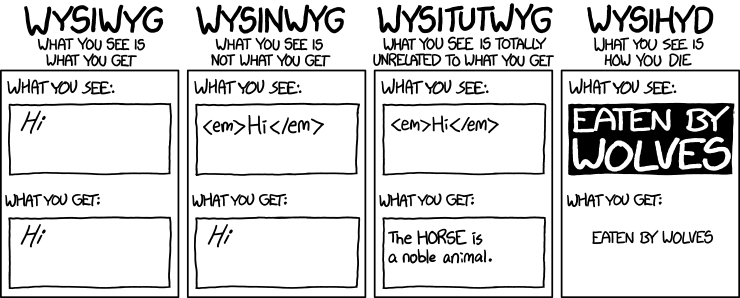
\includegraphics[scale=0.4]{Graphiques/types_of_editors}
				\caption{\href{http://xkcd.com/}{\copyright\ xkcd}}
				\label{Graphiques_editors}
			\end{figure}
		\end{center}
		

  		\subsection{Ins�rer une figure}

\tinycode
\begin{center}
	\begin{figure}
		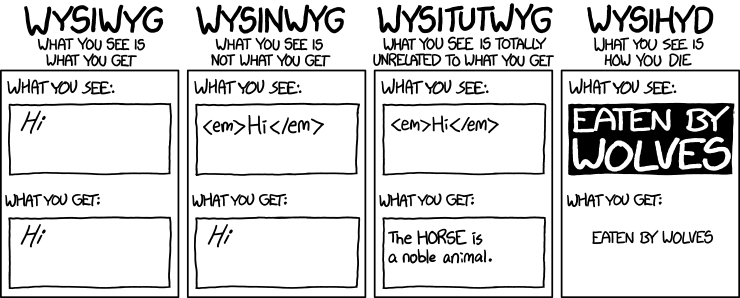
\includegraphics[scale=0.4]{Graphiques/types_of_editors}
		\caption{\href{http://xkcd.com/}{\copyright\ xkcd}}
		\label{Graphiques_editors}
	\end{figure}
\end{center}
\end{Verbatim}
		
		

			Pour les dimensions, il existe plusieurs arguments possibles~:
			
			\begin{description}
				\item[scale=] Dans ce cas on sp�cifie un rapport (de 0 � 1) d'agrandissement ou de r�duction
				\item[width=] On sp�cifie la largeur de l'image. La hauteur est recalcul� automatiquement
				\item[height=] On sp�cifie la hauteur de l'image. La hauteur est recalcul� automatiquement
				\item[width=,height=] La largeur et la hauteur de l'image sont sp�cifi�es.
				\item[keepaspectratio] quand on d�finit seulement une largeur ou une hauteur, cet argument permet de conserver le ratio largeur/hauteur original
			\end{description}

			D'autres arguments sont d�taill�s sur le \href{http://en.wikibooks.org/wiki/LaTeX/Importing_Graphics}{FramaBook} de Wikipedia.



\tinycode
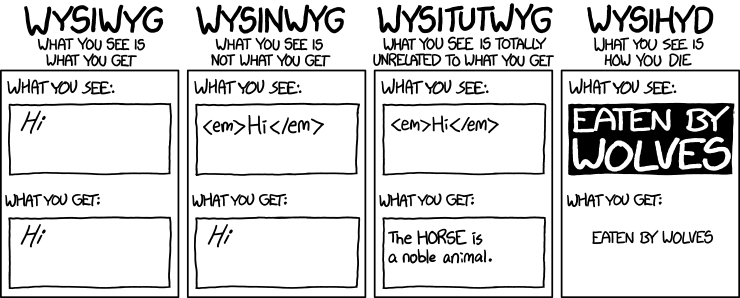
\includegraphics[scale=1]{Graphiques/types_of_editors} 
...
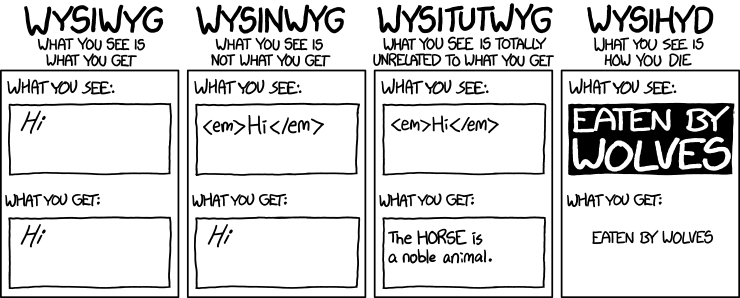
\includegraphics[width=0.5\textwidth]{Graphiques/types_of_editors}
...
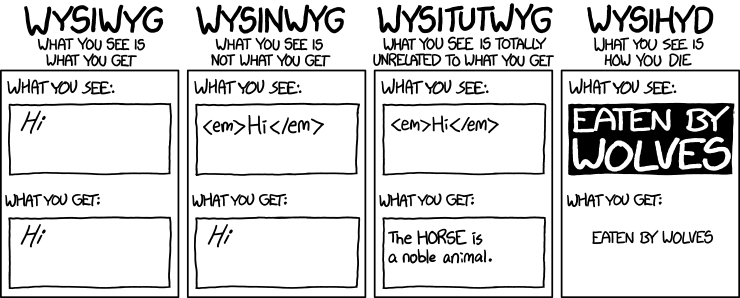
\includegraphics[width=0.5\textheight]{Graphiques/types_of_editors}
...
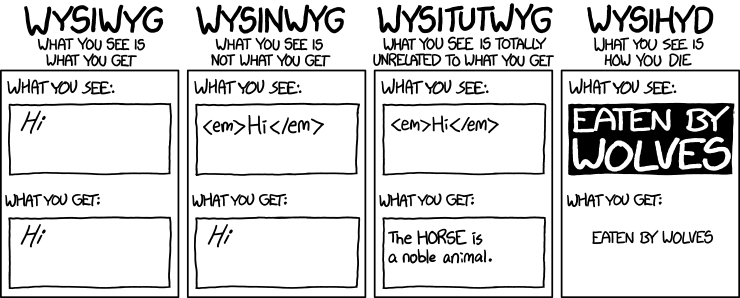
\includegraphics[width=0.5\textheight, height=0.5\textheight]{Graphiques/types_of_editors}
...
\end{Verbatim}
		
		
  		\subsection{Deux images cote � cote ?}

			Il suffit de m�langer les tableaux avec les images...
		
			\begin{center}		
				\begin{figure}
					\begin{tabular}{cc}
						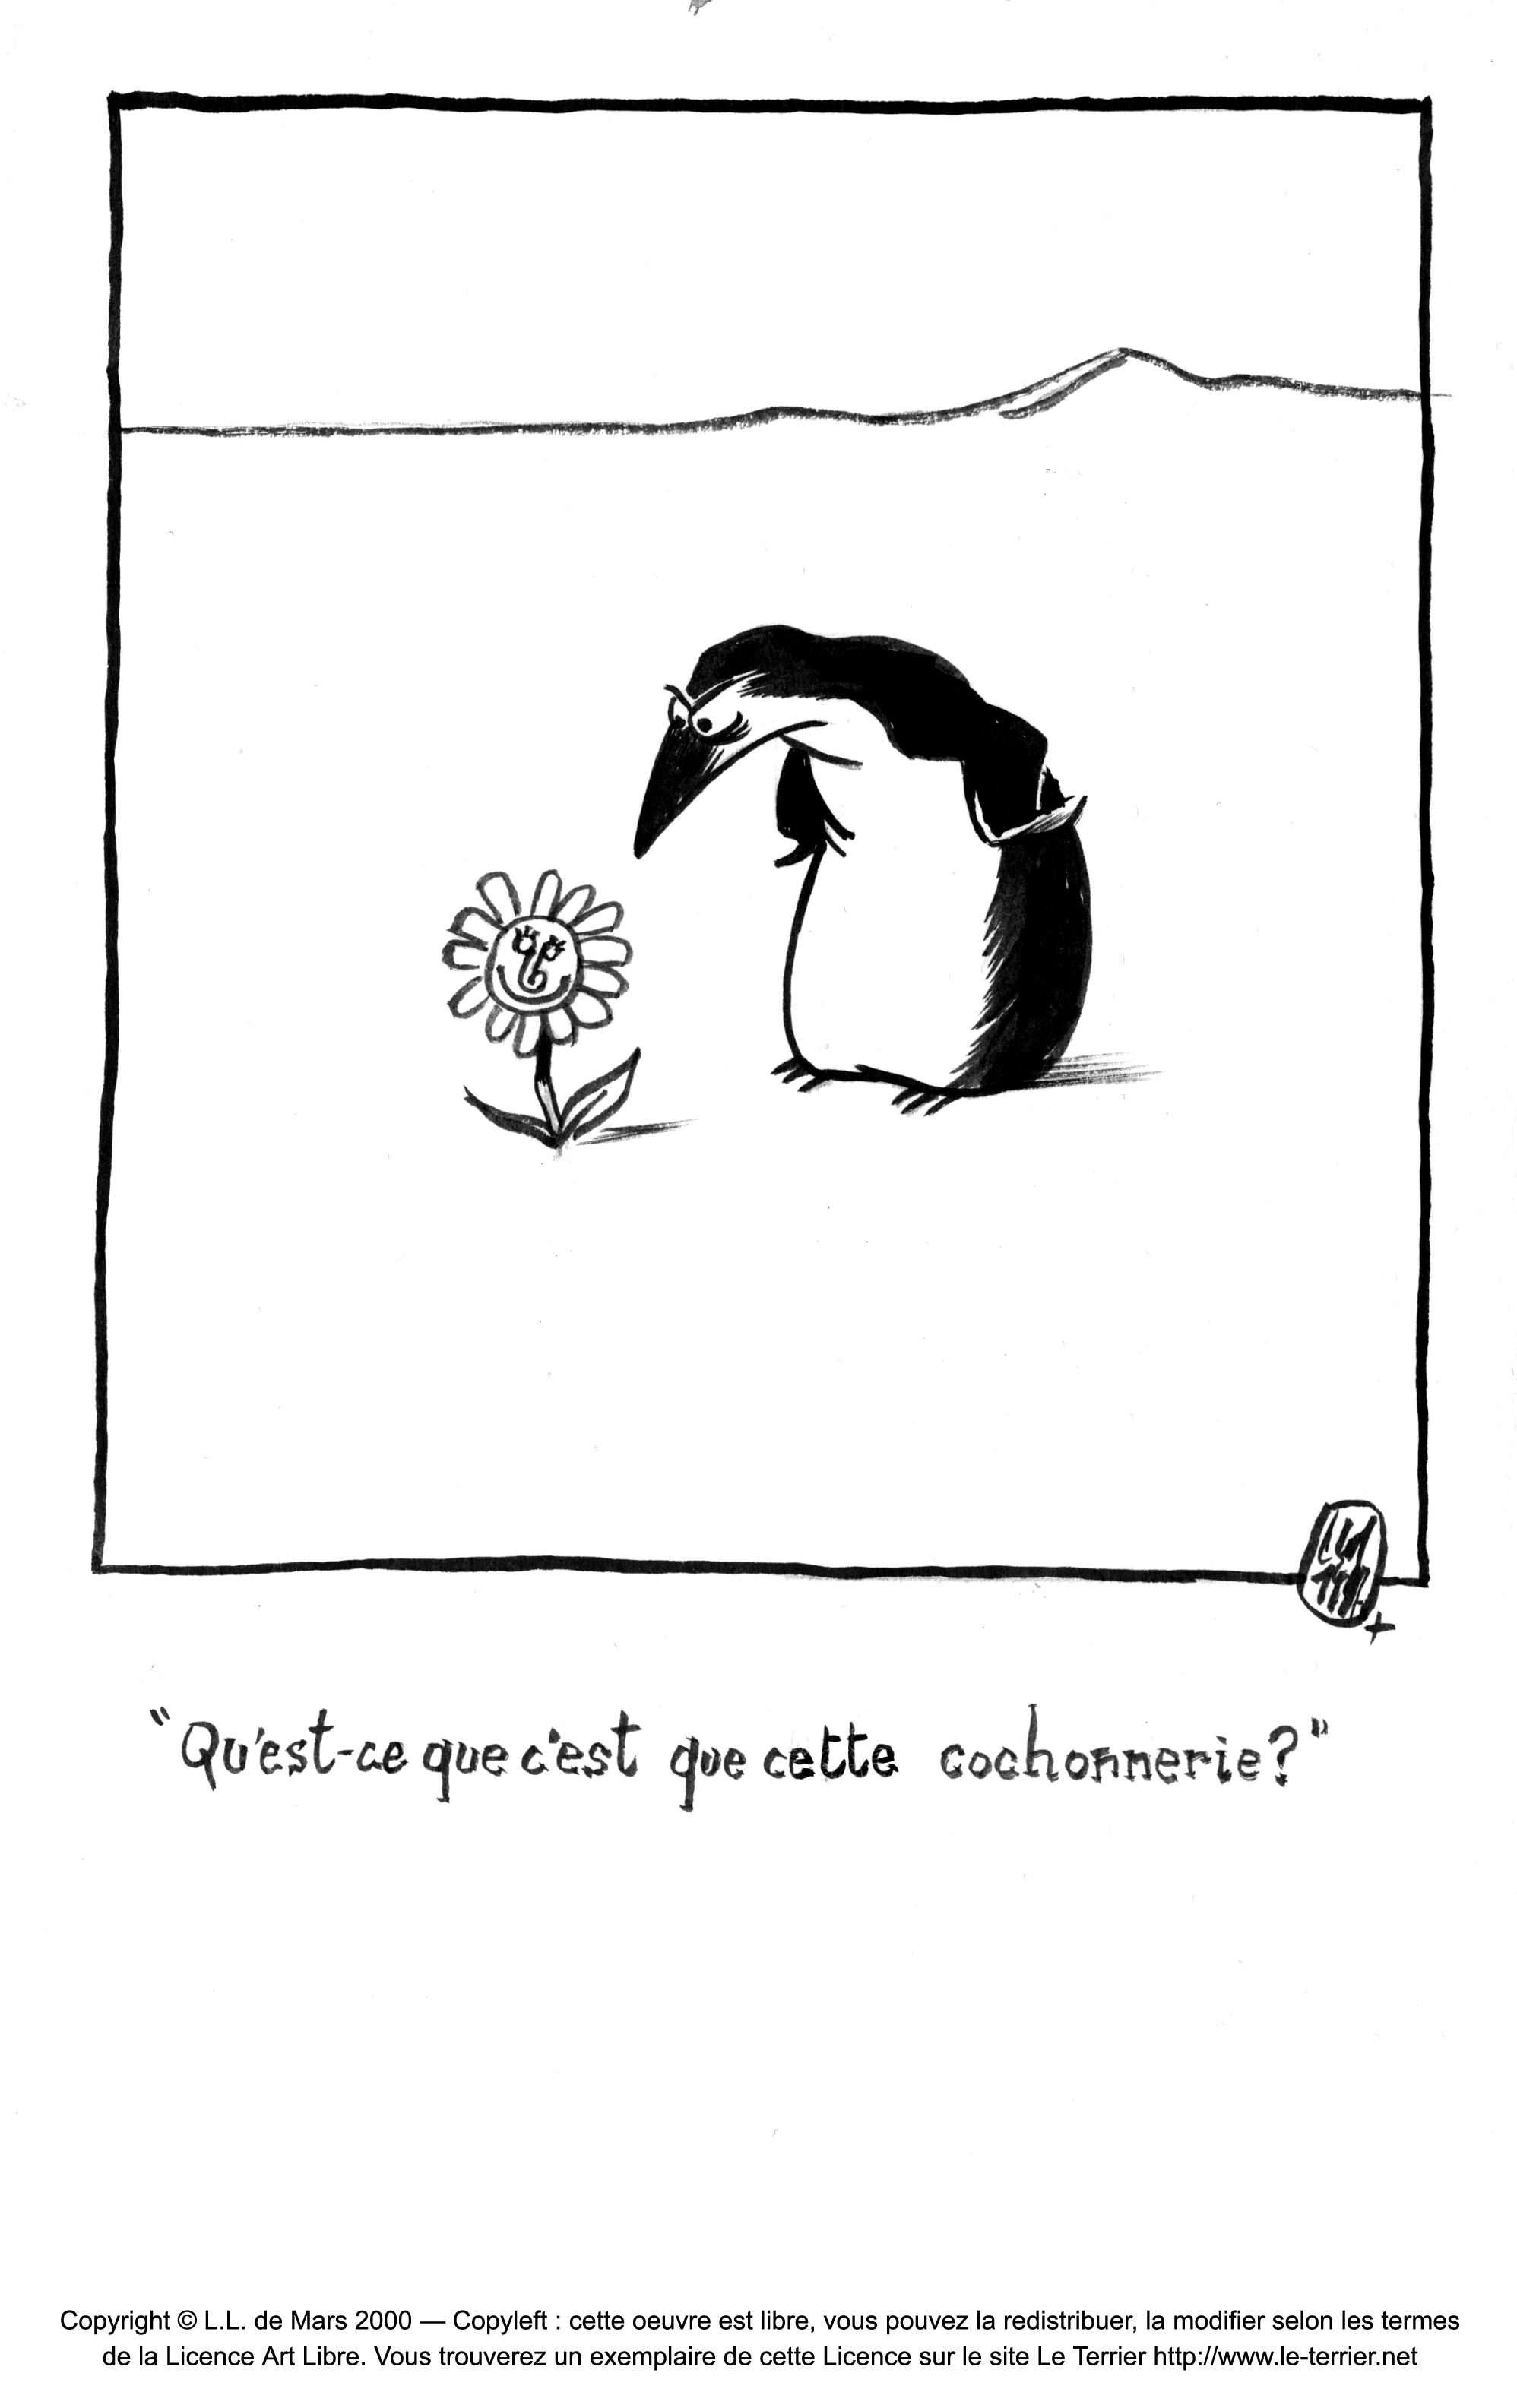
\includegraphics[scale=0.07]{Graphiques/3} 
						& 
						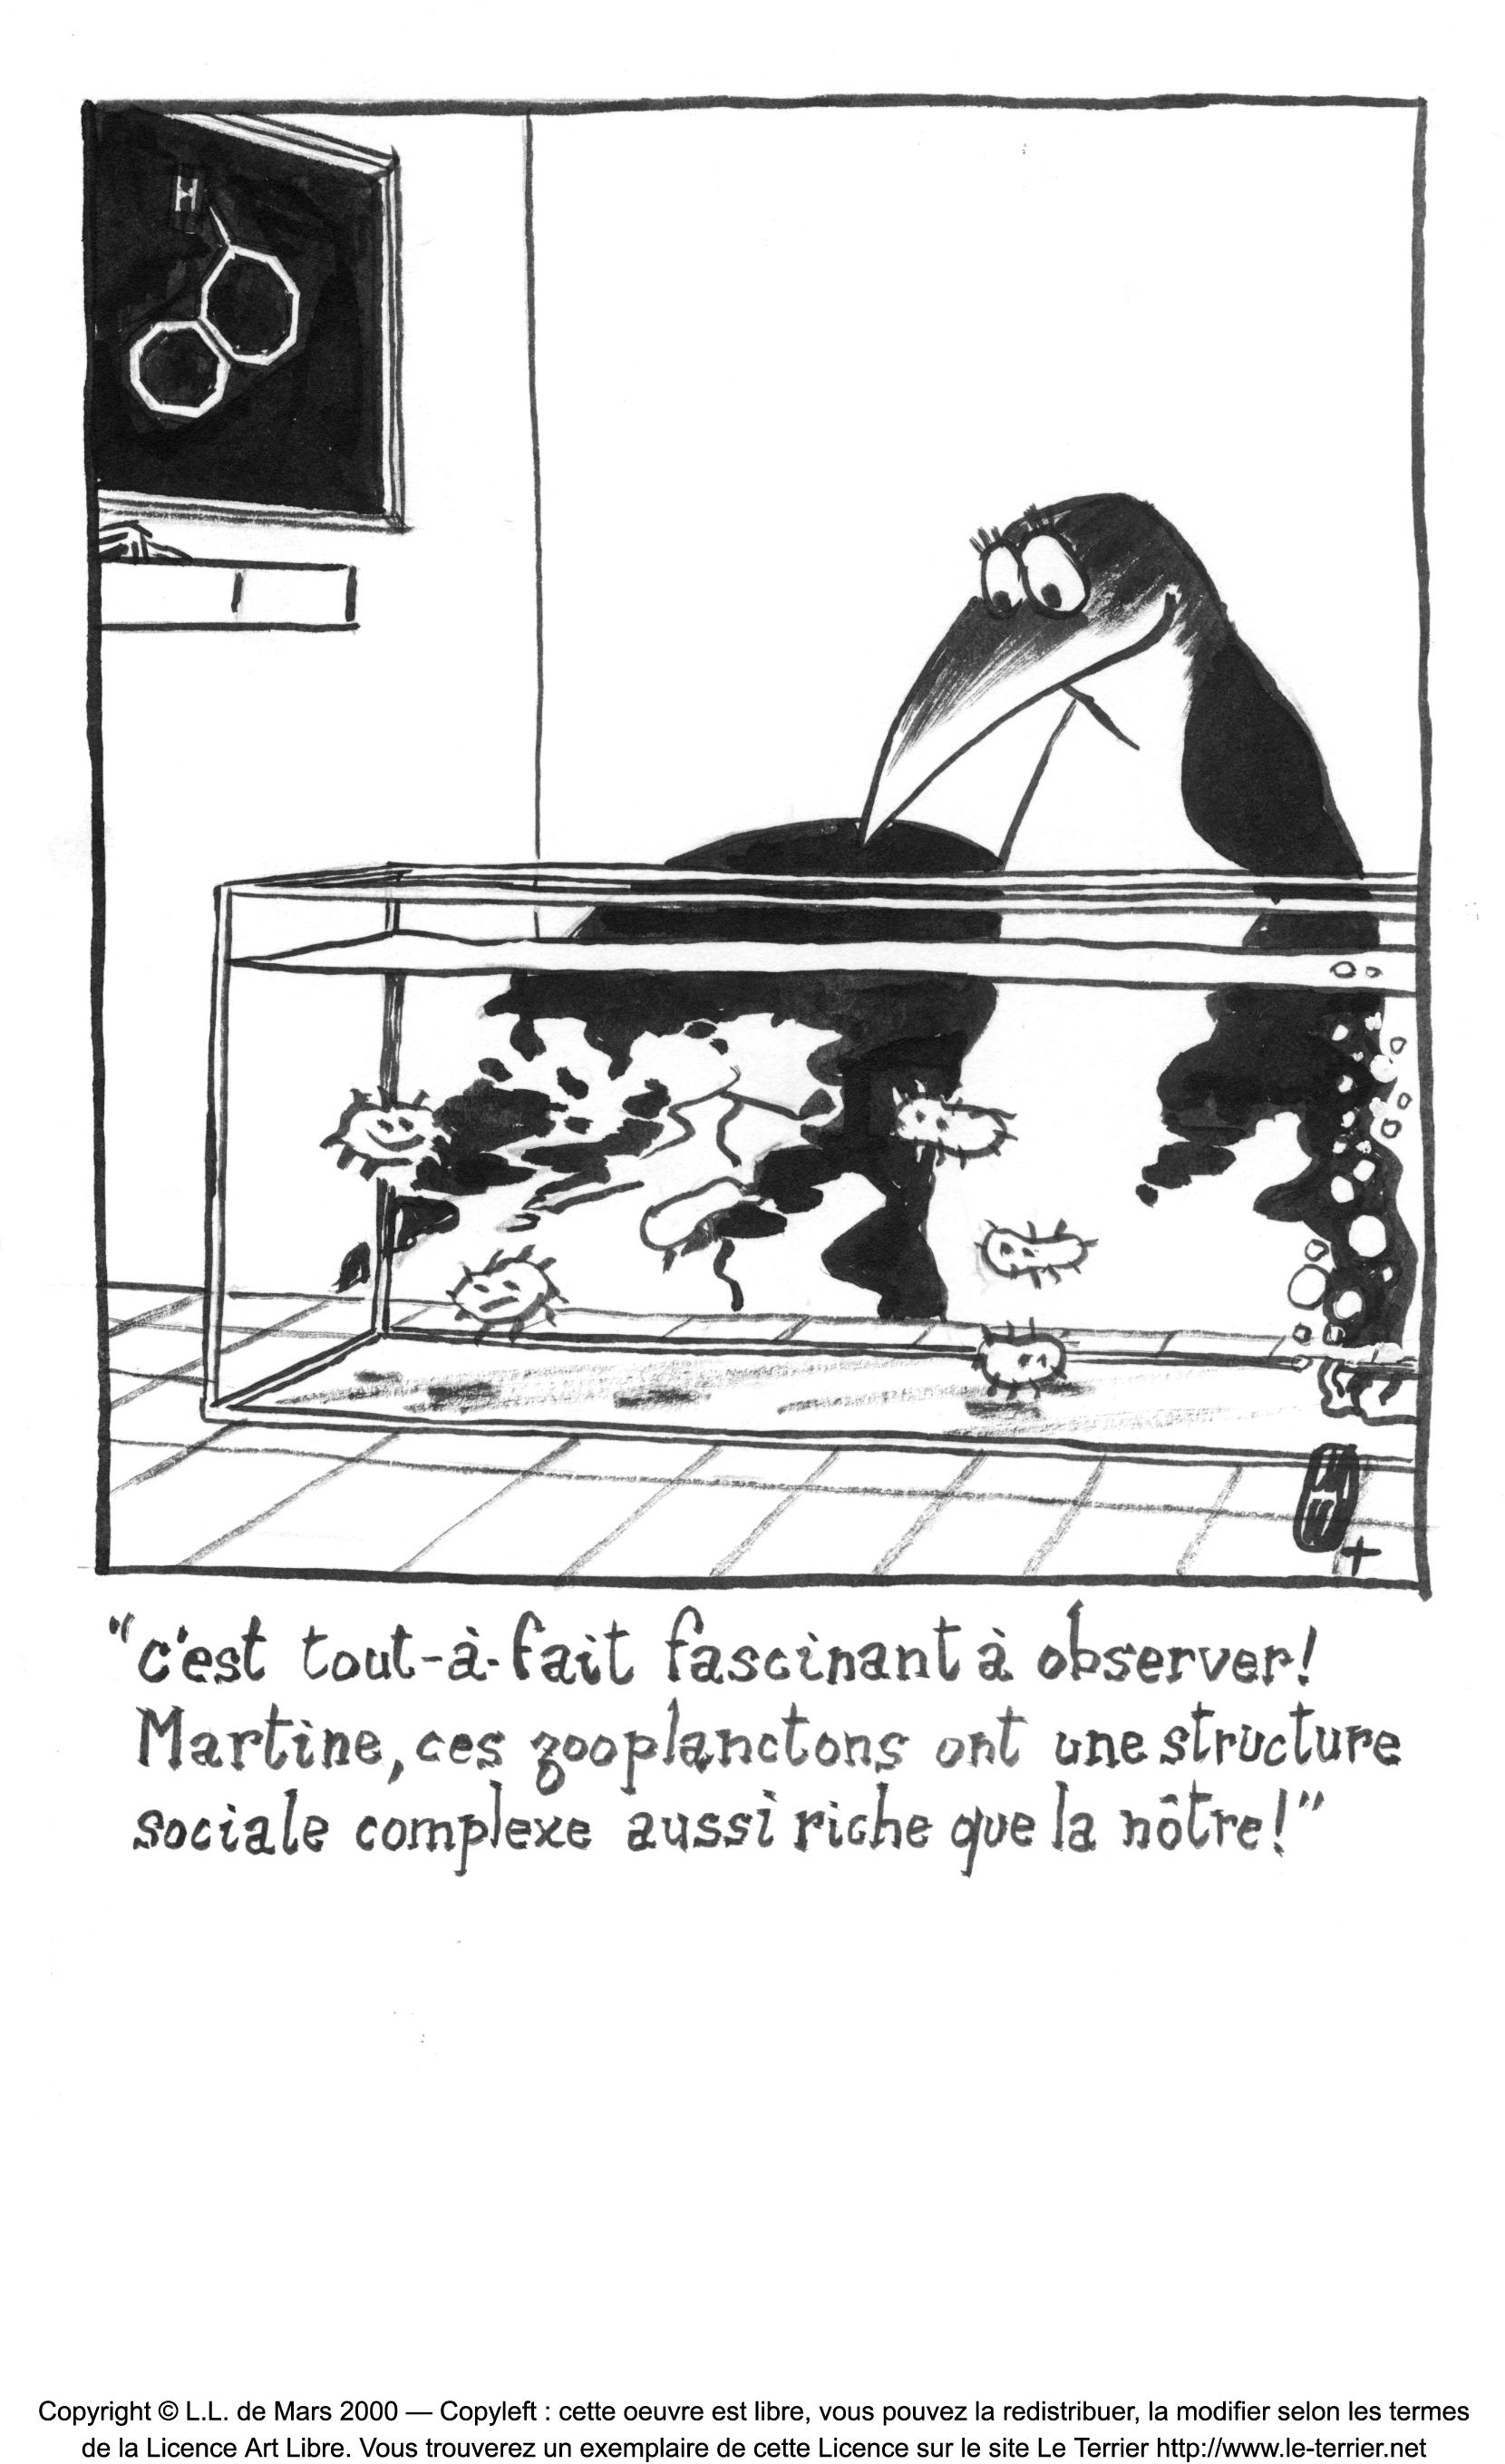
\includegraphics[scale=0.07]{Graphiques/29}\\
					\end{tabular}
					\caption{Les pingouins de L.L. deMArs}
					\label{Graphiques_Double}
				\end{figure}
			\end{center}



			Il suffit de m�langer les tableaux avec les images...

\tinycode			
\begin{center}		
	\begin{figure}
		\begin{tabular}{cc}
			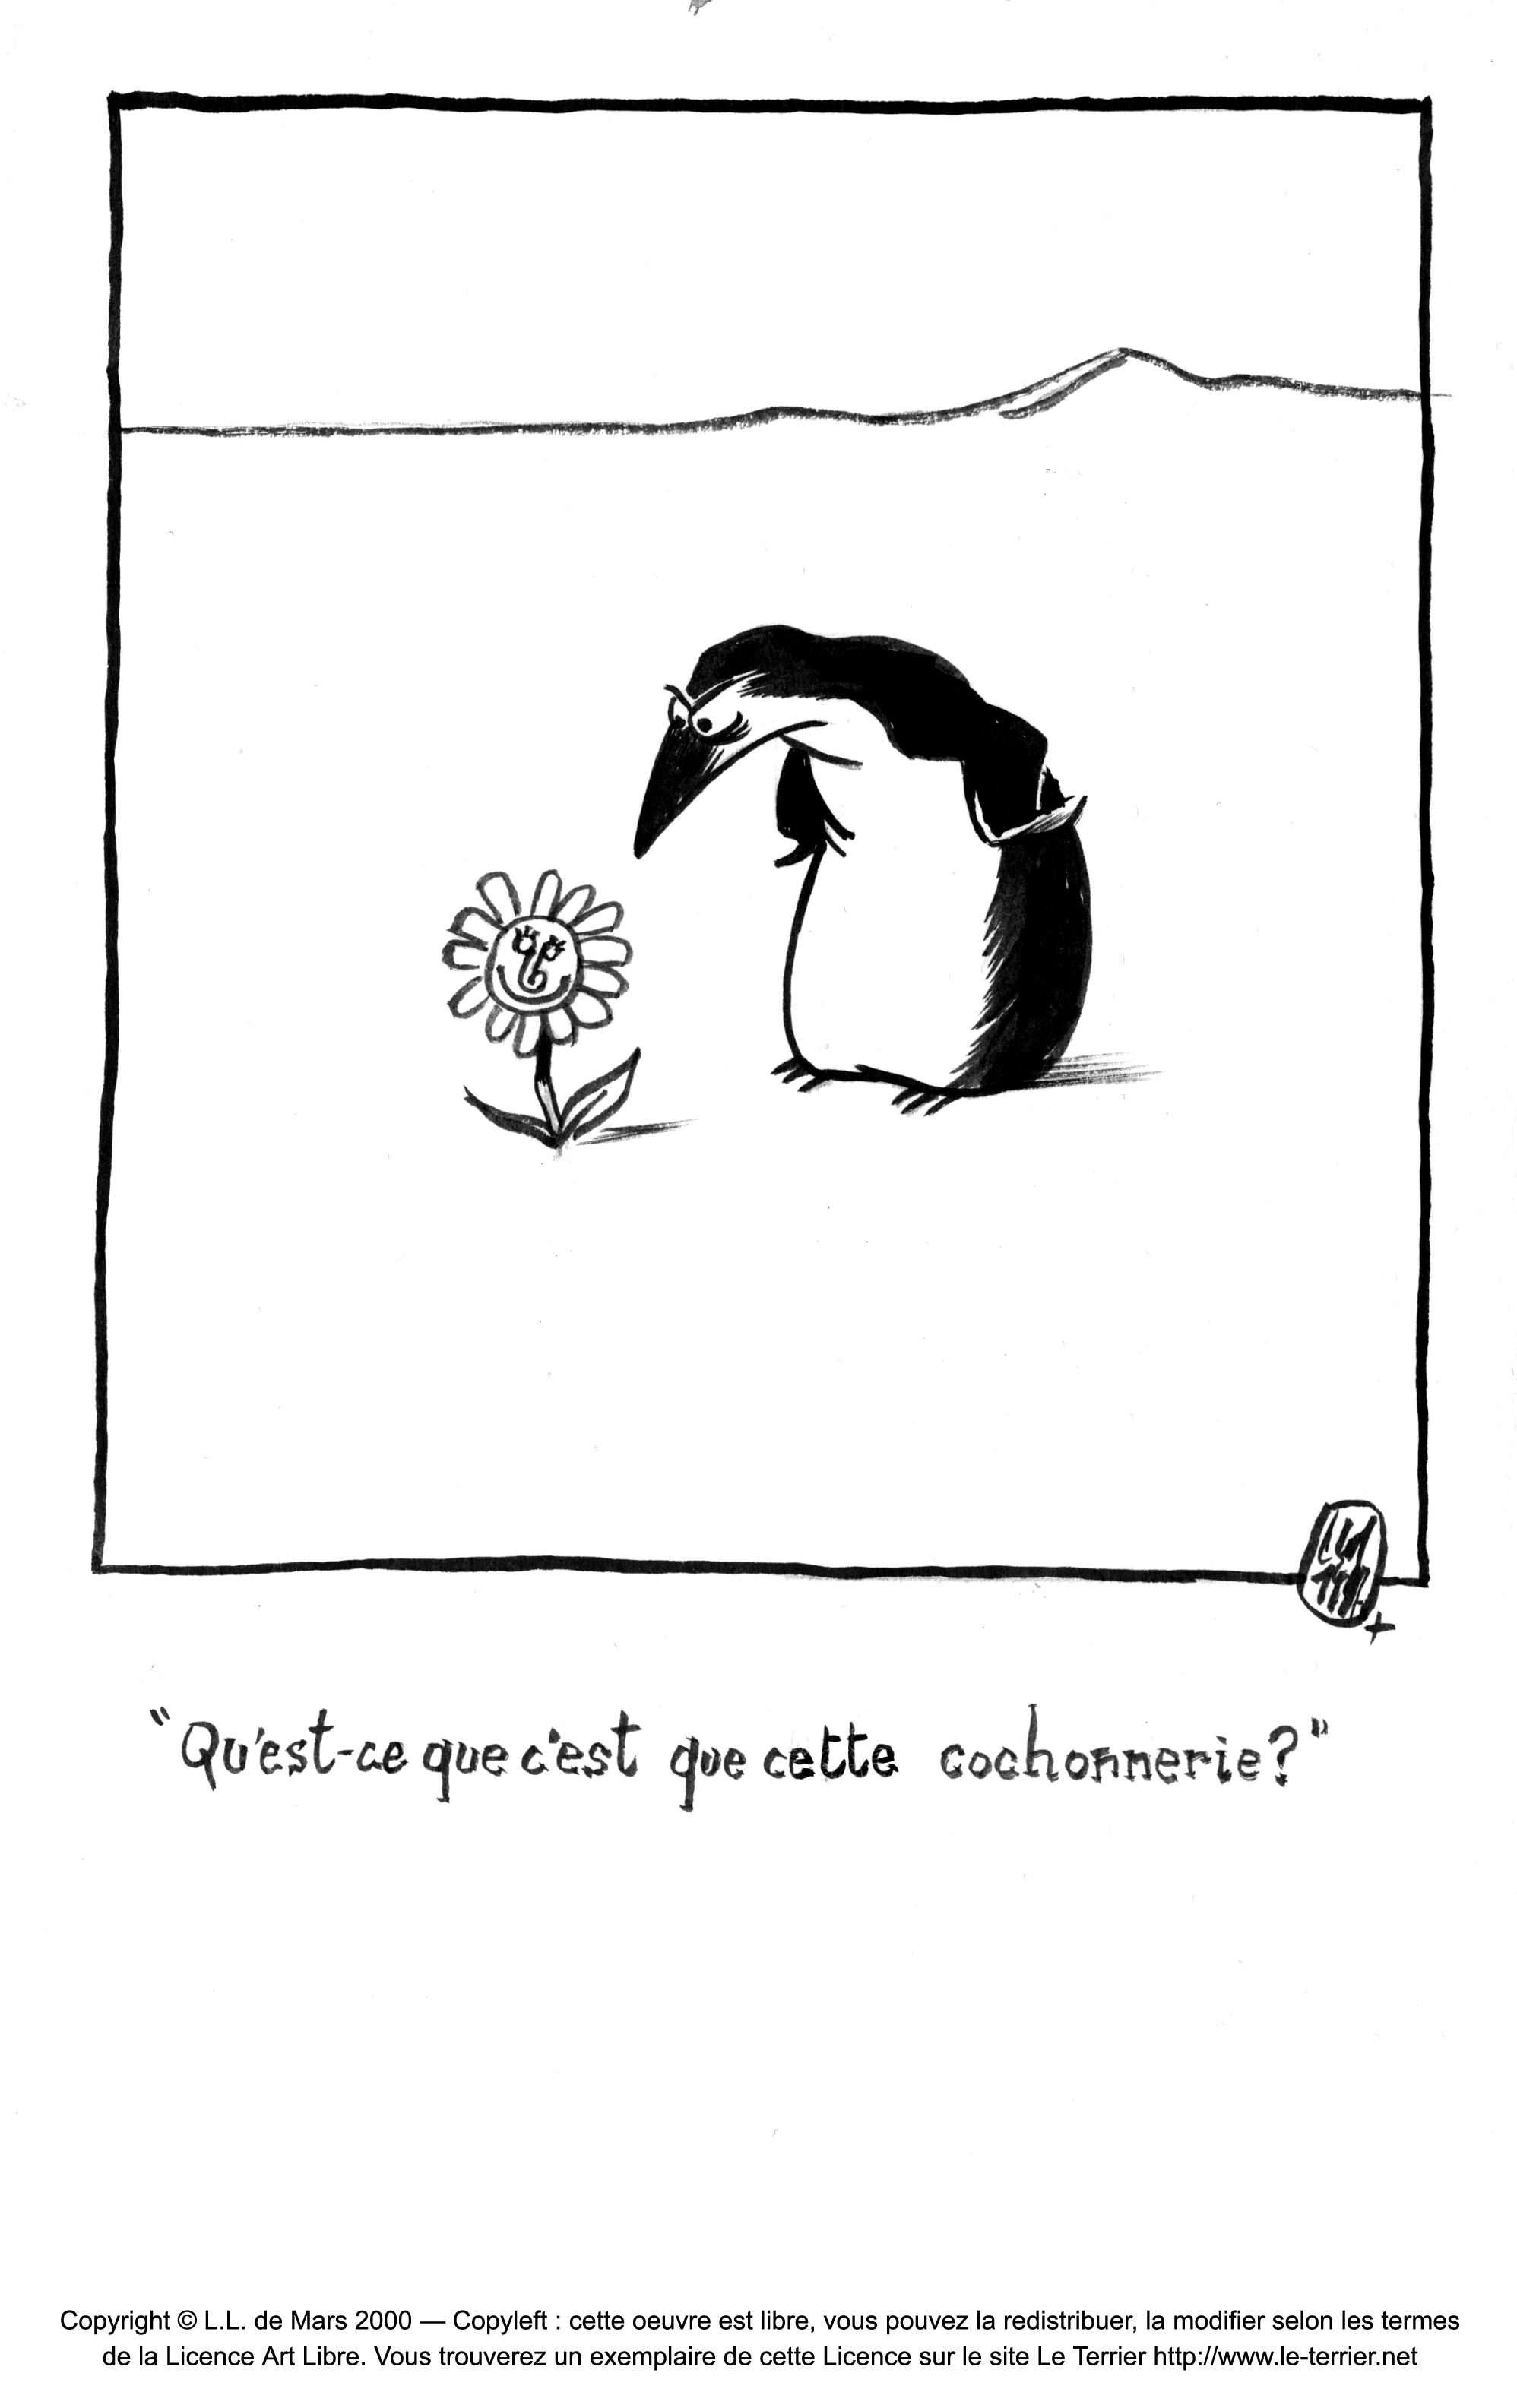
\includegraphics[scale=0.07]{Graphiques/3} 
			& 
			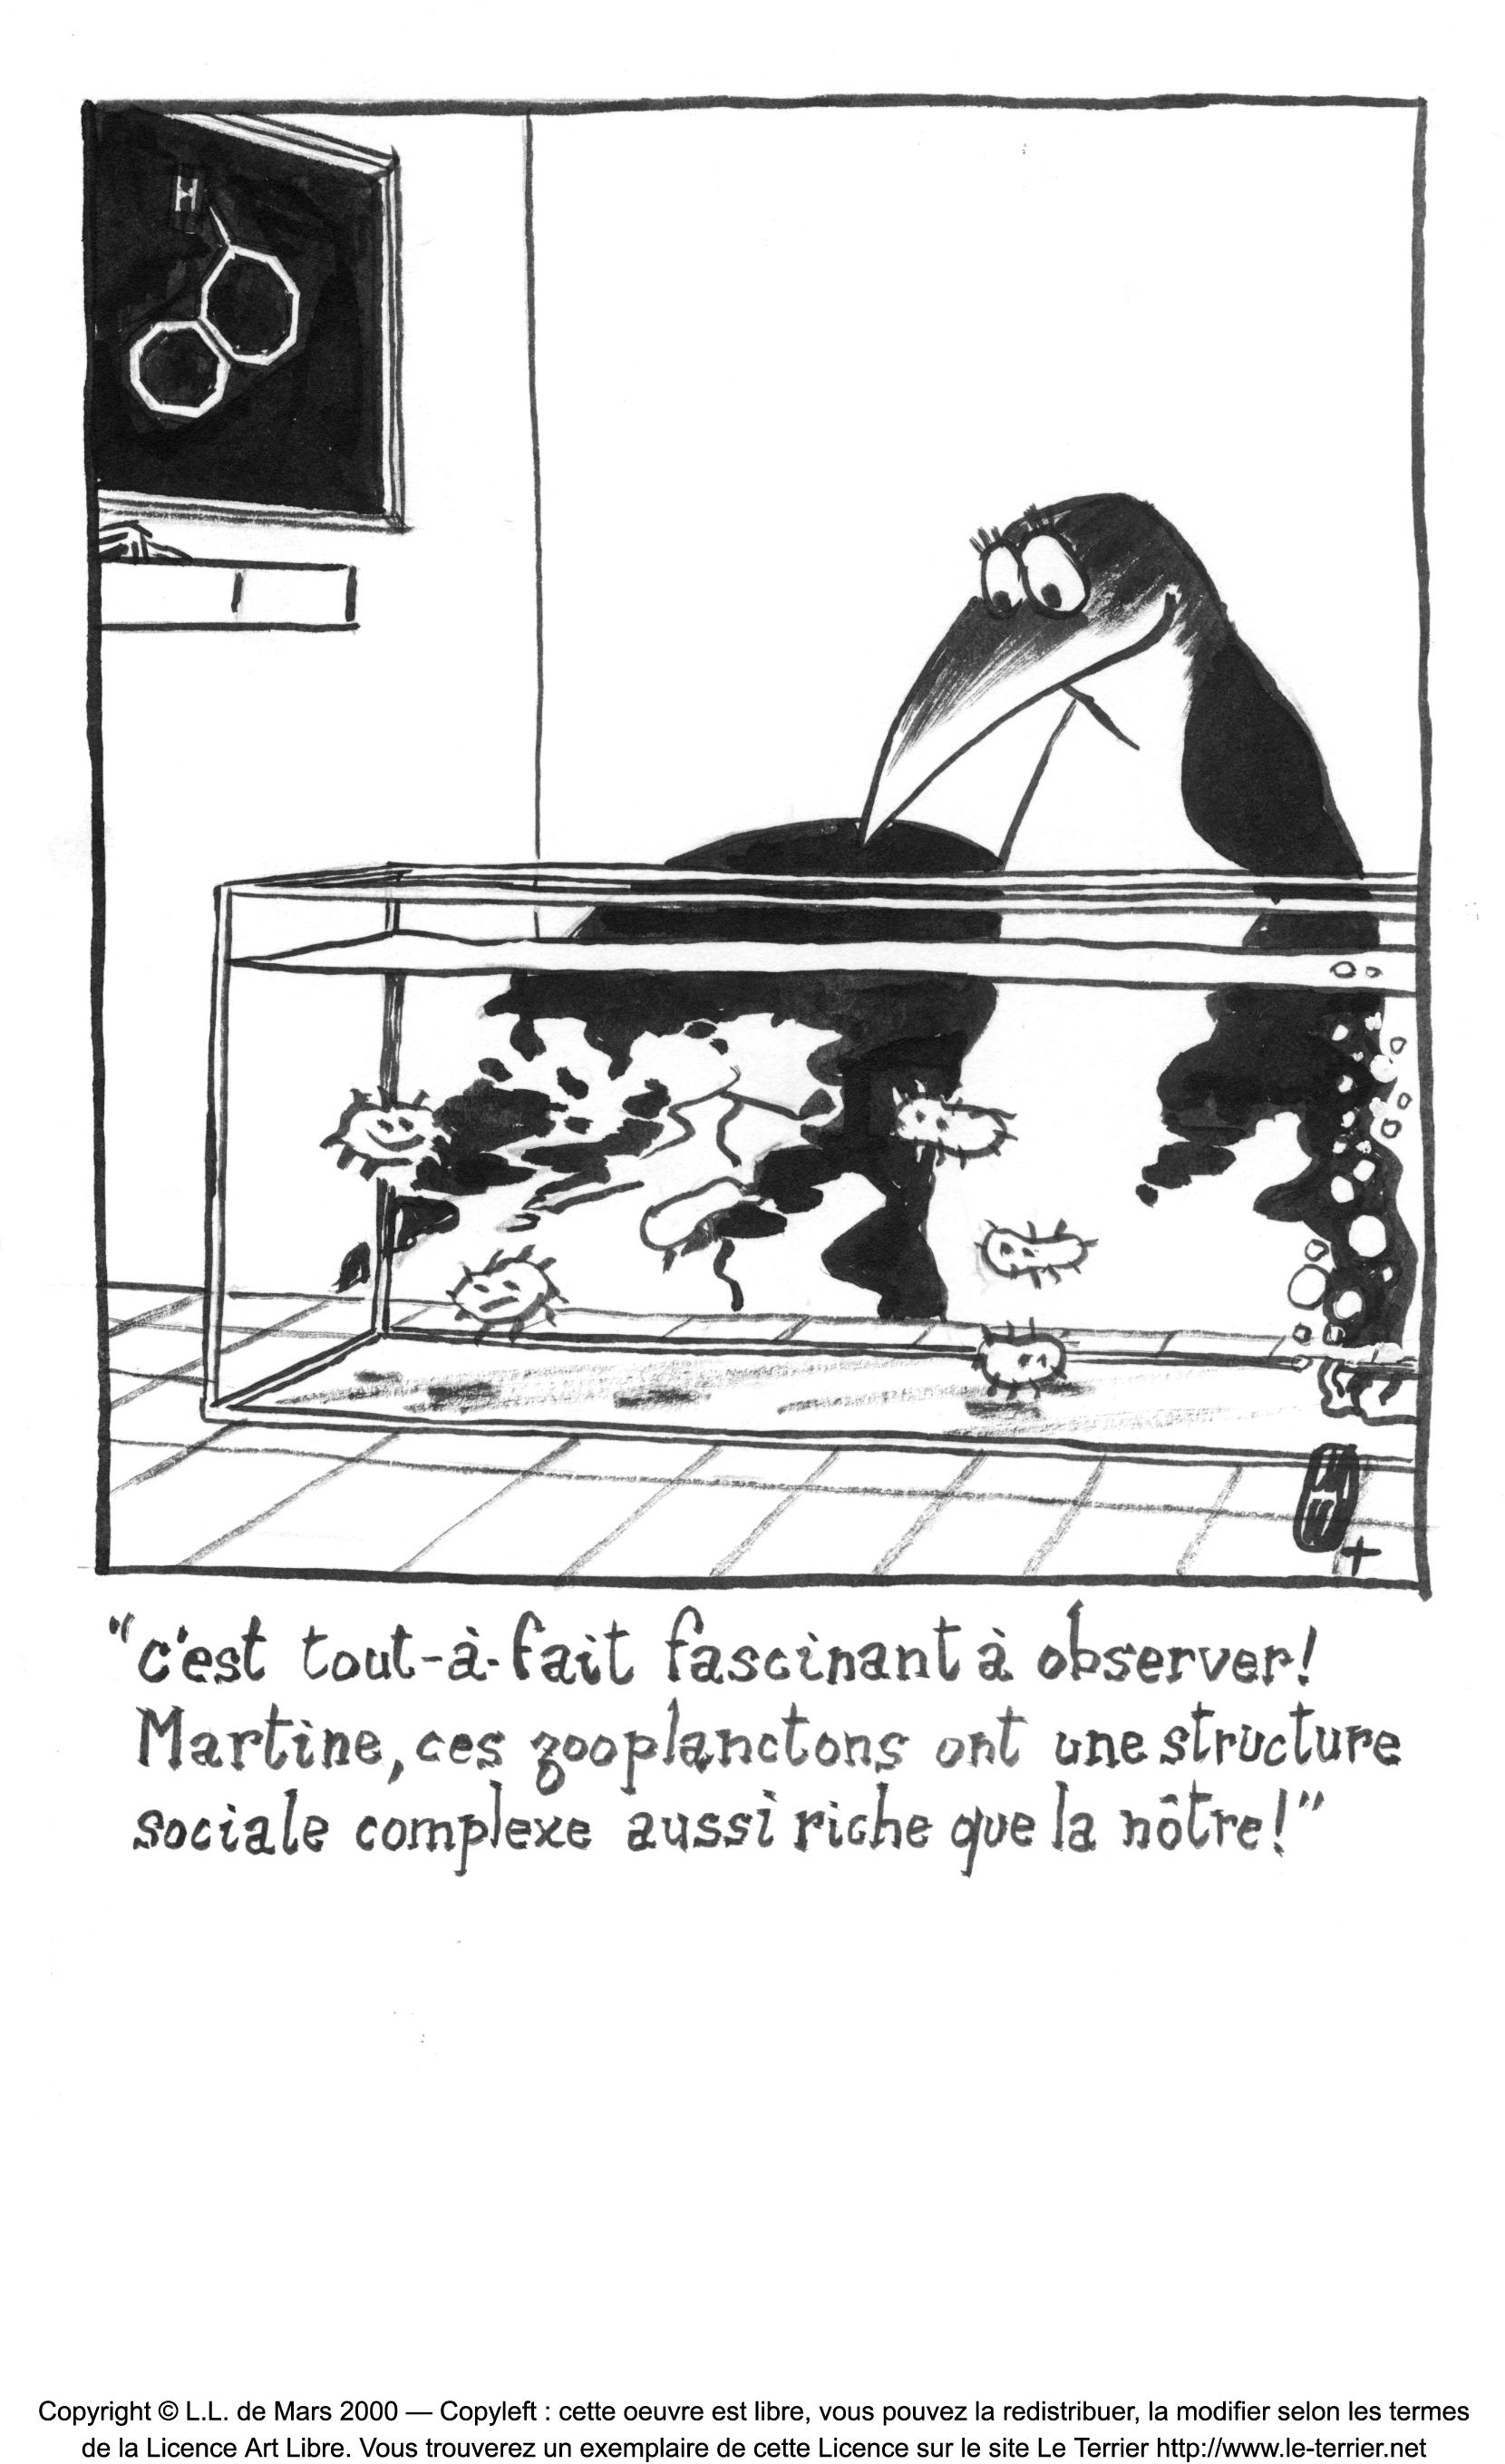
\includegraphics[scale=0.07]{Graphiques/29}\\
		\end{tabular}
		\caption{Les pingouins de L.L. deMArs}
		\label{Graphiques_Double}
	\end{figure}
\end{center}
\end{Verbatim}



  		\subsection{Des images de fond ou des logos...}

			Il est parfois n�cessaire d'ajouter une image de fond ou un logo.
			
			Ceci peut �tre r�alis� de nombreuses mani�res diff�rentes. Les plus communes sont d'utilis�s~:
			\begin{description}
				\item[le paquet \emph{watermark}] pour ins�rer un texte en filigrane
				\item[le paquet \emph{fancyhdr}] pour ins�rer des logos en bas et en haut de page
				\item[le paquet \emph{eso-pic}] pour ins�rer un filigrane, image de fond, un logo, ...
				\item[TikZ] pour ins�rer un filigrane, image de fond, un logo, ...
			\end{description}

						
			


\section{Listes � puce, ins�rer du code, ...}		

  	\subsection{Les listes \emph{� puces}}
			
			Les commandes de mise en page utilisent la syntaxe par blocs expliqu�e pr�c�demment.		  		

\code		  		
\begin{itemize}
	\item Num�ro 1
	\begin{itemize}	
		\item Num�ro 1
		\item Num�ro 2
	\end{itemize}	
	\item Num�ro 2
\end{itemize}
\end{Verbatim}
		
			Ce qui donne...	  		


			
			\begin{itemize}
				\item Num�ro 1
				\begin{itemize}	
					\item Num�ro 1
					\item Num�ro 2
				\end{itemize}						
				\item Num�ro 2
			\end{itemize}


			
			La syntaxe qui permet de changer le type de puce est assez simple.		  		

\code		  		
\begin{itemize}
	\item[\CheckmarkBold] Num�ro 1
	\begin{itemize}	
		\item[\ding{51}] Num�ro 1
		\item[\ding{56}] Num�ro 2
	\end{itemize}	
	\item[\XSolidBrush] Num�ro 2
\end{itemize}
\end{Verbatim}
		
			Ce qui donne...	  		


			
		\begin{itemize}
			\item[\CheckmarkBold] Num�ro 1
			\begin{itemize}	
				\item[\ding{51}] Num�ro 1
				\item[\ding{56}] Num�ro 2
			\end{itemize}	
			\item[\XSolidBrush] Num�ro 2
		\end{itemize}


			
			Les quelques lignes pr�c�dentes pose le probl�me de trouver la liste des symboles de \latex. 
			
			Comme �voqu� pr�cedemment, le lecteur trouvera sont bonheur dans la liste des caract�res sp�ciaux r�unis dans le document \href{http://www.ctan.org/tex-archive/info/symbols/comprehensive/}{\emph{The Comprehensive \latex Symbol List}}.
			
			L'ouvrage \href{http://framabook.org/5-tout-ce-que-vous-avez-toujours-voulu-savoir-sur-latex-sans-jamais-oser-le-demander/}{FramaBook \LaTeX} de l'association \emph{Framasoft} est �galement une source d'inspiration.
			

  	\subsection{Les listes decriptives}
		

\begin{description}
	\item[\TeX] Le langage original par Knuth
	\item[\LaTeX] La version �volu�e et plus simple.
	\item[Con\TeX] Une version tr�s int�ressante 
\end{description}


		

				
		
			\code	
\begin{description}
	\item[\TeX] Le langage original par Knuth
	\item[\LaTeX] La version �volu�e et plus simple.
	\item[Con\TeX] Une version tr�s int�ressante 
\end{description}
			\end{Verbatim}

		

		
			
  	\subsection{Les listes incr�ment�es}
			
			\code		  		
\begin{enumerate}
	\item Num�ro 1
	\begin{enumerate}
		\item Num�ro 1 
		\item Num�ro 1
	\end{enumerate}
	\item Num�ro 2
\end{enumerate}
			\end{Verbatim}
		
			Ce qui donne...	  		


			
		\begin{enumerate}[1.]
			\item Num�ro 1
			\begin{enumerate}[1.]
				\item Num�ro 1 
				\item Num�ro 1
			\end{enumerate}
			\item Num�ro 2
		\end{enumerate}



		Il y a la possbilit� de changer le style de num�rotation~:

		\begin{description}
			\item [Brutale] en utilisant l'environnement 
			\item [paquet \emph{enumitem}] Les commandes disponibles dans ce paquet sont notamment~: 
					\begin{description}
						\item[\textbackslash alph\{number\}] lettres en minuscules
						\item [\textbackslash Alph\{number\}] lettres en majuscules
						\item [\textbackslash arabic\{number\}] les nombres
						\item [\textbackslash roman\{number\}] des lettres \og~romaines~\fg en minusucules et des num�ros
						\item [\textbackslash Roman\{number\}] des lettres \og~romaines~\fg en majusucules et des num�ros
					\end{description}
					
		\end{description}
			

			
			\code		  		
\begin{enumerate}[label=\arabic{*})]
	\item Num�ro 1
	\begin{enumerate}[label=\alph{*})]
		\item Num�ro 1 
		\item Num�ro 1
	\end{enumerate}
	\item Num�ro 2
\end{enumerate}
			\end{Verbatim}
		

 	
		\begin{description}
			\item [paquet \emph{enumerate}] qui a une syntaxe plus naturelle mais qui pr�sente moins de possibilit�s...
				\vspace{0.3cm}
				\code
\begin{enumerate}[a)]
\item ...
\end{enumerate}			
				\end{Verbatim}
		\end{description}



\begin{enumerate}[1)]
	\item Num�ro 1
	\begin{enumerate}[a)]
		\item Num�ro 1 
		\item Num�ro 1
	\end{enumerate}
	\item Num�ro 2
\end{enumerate}

		

		Pour commencer (ou plut�t reprendre) une liste num�rot�e en cours de route, il faut jouer sur la valeur du compteur. Les compteurs d�crit plus loin sont des variables incr�ment�es par \latex et/ou par l'utilisateur.
		
		\code
\begin{enumerate}[1)]
	\setcounter{enumi}{5}
	\item Num�ro 1
	\begin{enumerate}[a)]
		\setcounter{enumii}{3}
		\item Num�ro 1 
		\item Num�ro 1
	\end{enumerate}
	\item Num�ro 2
\end{enumerate}
\end{Verbatim}
	


\begin{enumerate}[1)]
	\setcounter{enumi}{5}
	\item Num�ro 1
	\begin{enumerate}[a)]
		\setcounter{enumii}{3}
		\item Num�ro 1 
		\item Num�ro 1
	\end{enumerate}
	\item Num�ro 2
\end{enumerate}
	


 	\subsection{Encore plus de listes...}

	Les paquets \emph{inparaenum}, \emph{enumitem}, \emph{easylist}, \ldots permettent de nombreuses fonctionnalit�s autour des listes.

	Par exemple, \emph{paralist} permet d'ajouter une liste num�rot�e � l'int�rieur d'un texte.
	

\section{Justification, taille et couleur du texte}				

  	\subsection{Justifions du texte...}
			
			Toujours par blocs...
			
			\code
\begin{right}		  		
	Ce texte est � droite...\\
\end{right}
\begin{center}		  		
	Ce texte est centr�...\\
\end{center}
\begin{left}		  		
	Ce texte est � gauche...\\
\end{left}
			\end{Verbatim}
			
			Ce qui donne...


			
			\begin{flushright}		  		
			Ce texte est � droite...\\
			\end{flushright}
			\begin{center}		  		
			Ce texte est centr�...\\
			\end{center}
			\begin{flushleft}		  		
			Ce texte est � gauche...\\
			\end{flushleft}
			


  		\subsection{Justification du texte}

                Vous pouvez souhaiter justifier du texte comme \textit{Word} avec l'option "ligne pleine"~: c'est-�-dire avec le moins d'espace possible et aucun mot ne d�passant et aucune c�sure. Dans ce cas, il faut int�grer le code ci-dessous dans le pr�ambule o� dans un bloc. 

\code
\tolerance=1
\emergencystretch=\maxdimen
\hyphenpenalty=10000
\hbadness=10000
\end{Verbatim}


  	\subsection{Mettons en �vidence...}

			\begin{table}[h!]
			\begin{center}
			  {\setlength{\extrarowheight}{4pt}
			  \begin{tabular}{|l|l|c|}
			    \hline
			    \hfil Commande      & \hfil D\'eclarations   & Output \\
			    \hline
			    \ltxcom{textrm}\verb+{...}+ & 
			    \verb+{+\ltxcom{rmfamily}\verb+ ...}+ & {\rmfamily roman}\\
			    \ltxcom{textsf}\verb+{...}+ & 
			    \verb+{+\ltxcom{sffamily}\verb+ ...}+ & {\sffamily sans s�rif}\\
			    \ltxcom{texttt}\verb+{...}+ & 
			    \verb+{+\ltxcom{ttfamily}\verb+ ...}+ & {\ttfamily machine � �crire}\\
			    \hline
			    \ltxcom{textup}\verb+{...}+ & 
			    \verb+{+\ltxcom{upshape}\verb+ ...}+ & {\upshape droit}\\
			    \ltxcom{textit}\verb+{...}+ & 
			    \verb+{+\ltxcom{itshape}\verb+ ...}+ & {\itshape italique}\\
			    \ltxcom{textsl}\verb+{...}+ & 
			    \verb+{+\ltxcom{slshape}\verb+ ...}+ & {\slshape pench�}\\
			    \ltxcom{textsc}\verb+{...}+ & 
			    \verb+{+\ltxcom{scshape}\verb+ ...}+ & {\scshape Petites Capitales}\\
			    \hline
			    \ltxcom{textmd}\verb+{...}+ & 
			    \verb+{+\ltxcom{mdseries}\verb+ ...}+ & {\mdseries medium}\\
			    \ltxcom{textbf}\verb+{...}+ & 
			    \verb+{+\ltxcom{bfseries}\verb+ ...}+ & {\bfseries gras}\\
			    \hline
			  \end{tabular}}
                        \caption{tir� du FramaBook sur \LaTeX}
			\end{center}  
			\end{table}



			Cette fois c'est une commande avec arguments...
  	
  	\code
Ce texte est en mode normal\\
\emph{Ce texte est en italique}\\
\texttt{Ce texte est en machine � �crire}\\
\textit{Ce texte est en italique}\\
\textsc{Ce texte est en petites capitales}\\
\textbf{Ce texte est en gras}\\
  	\end{Verbatim}
		
		ce qui donne...  	


  	
  		Ce texte est en mode normal\\
	  	\emph{Ce texte est mis en �vidence}\\
	  	\texttt{Ce texte est en machine � �crire}\\
	  	\textit{Ce texte est en italique}\\
	  	\textsc{Ce texte est en petites capitales}\\
	  	\textbf{Ce texte est en gras}\\



  	\code
{ \bfseries Cette syntaxe diminue notablement la 
lisibilit� du code.
} 
  	\end{Verbatim}
  	
  	{ \bfseries Donc � utiliser avec pr�caution. }


  	\subsection{Mettons en couleurs...}
  	
  		Dans ce cas, on appelle une macro dans le paquet \emph{color}. Du coup, l'appel se fait par la commande suivie de plusieurs accolades, chaque couple d'accolade abritant un argument~: 
  	\code
\textcolor{red}{...texte...}
  	\end{Verbatim}
		
  	\textcolor{red}{L'appel se fait avec la couleur en premier argument puis le texte � coloriser dans le second argument.}
  	
		
  	\subsection{Les tailles de polices...}
		
		Pour les tailles de police, c'est une commande sans argument qui va changer l'interpr�tation du texte qui la suit~: 
		
  	\code
\Huge Lorem ipsum \LARGE dolor sit amet, consectetur 
\normalsize adipiscing elit. \tiny Nunc in dui nec arcu 
\normalsize facilisis cursus id nec lorem.   	
\end{Verbatim}
		

		
		Ce qui donne...
		
\Huge Lorem ipsum \LARGE dolor sit amet, consectetur 
\normalsize adipiscing elit. \tiny Nunc in dui nec arcu 
\normalsize facilisis cursus id nec lorem.   	
		



			\begin{table}[h!]
			  \caption{Changement de taille (Tir� du Framabook sur \LaTeX)}
			  \label{tab-taille}
			  \begin{center}
			    {\addtolength{\extrarowheight}{4pt}
			    \begin{tabular}{||l|c||l|c||}
			      \hline
			      \ltxcom{Huge} & {\Huge immense} & \ltxcom{normalsize} & {\normalsize normal} \\
			      \ltxcom{huge} & {\huge �norme} & \ltxcom{small} & {\small petit}
			      \\
			      \ltxcom{LARGE}& {\LARGE tr�s tr�s gros} &  \ltxcom{footnotesize}& {\footnotesize plus petit} \\
			      \ltxcom{Large} & {\Large tr�s gros} &  \ltxcom{scriptsize}  & {\scriptsize encore plus petit} \\
			      \ltxcom{large} & {\large gros}  & \ltxcom{tiny} & {\tiny
			        minuscule} \\
			      \hline
			    \end{tabular}}
			  \end{center}
			\end{table}		

				
\section{Ajout d'espacement et autres...}		
		
  		\subsection{Espacement vertical}
  		
  		Pour forcer \latex � ins�rer un espace entre deux paragraphes, il faut utiliser la commande \textbackslash vspace.
  		
  		\code
Du texte...\\
\vspace{1cm}
Le reste du texte...
\end{Verbatim}

Du texte...\\
\vspace{1cm}
Le reste du texte...
		

  		\subsection{Espacement horizontal}
  		
  		Pour forcer \LaTeX � ins�rer un espace entre deux mots, il faut utiliser la commande \textbackslash hspace.
  	
  		\code
Du texte...\hspace{1cm}Le reste du texte...
\end{Verbatim}

Du texte...\hspace{1cm}Le reste du texte...
		
		
  		\subsection{Ins�rer une ligne}
  		
  		Pour ins�rer une ligne horizontale, il suffit d'appeler la commande \textbackslash hrule.
  		
  		\code
  		Du texte...\\
			\vspace{0.1cm}
  		\hrule
  		\vspace{0.1cm}
  		Le reste du texte...
  		\end{Verbatim}
		
  		Du texte...\\
			\vspace{0.1cm}
  		\hrule
  		\vspace{0.1cm}
  		Le reste du texte...
		


  		
  		Dans le m�me genre d'id�es...
  		
  		\code
Du texte \dotfill du texte \dotfill du texte\\
\vspace{0.1cm}
Du texte \hrulefill du texte \hrulefill du texte\\
  		\end{Verbatim}
		
Du texte \dotfill du texte \dotfill du texte\\
\vspace{0.1cm}
Du texte \hrulefill du texte \hrulefill du texte\\
		
		
  		\subsection{Ins�rer des sauts de page}
  		
  		Pour ins�rer un saut de page manuel, il suffit d'ajouter \emph{\textbackslash newpage}.
  		
  		La commande \emph{\textbackslash clearpage} est l�g�rement diff�rentes~: elle indique au compilateur qu'un saut de page est n�cessaire mais elle impose aussi au compilateur de vider le tampon contenant les flottants. Par cons�quent tous les tableaux et toutes les figures \fg~en attente~\fg sont plac�s dans le document au niveau de la commande. 
  		
  		La commande \emph{\textbackslash clearpage} s'utilise typiquement quand on veut un saut de page entre le chapitre 2 et le chapitre 3. De plus, les figures du chapitre 2 ne doivent pas appara�tre dans le chapitre 3.
  		  		

\section{Mise en page}

  		\subsection{Red�finir les marges et l'espace imprimable...}

		Cela peut �tre r�alis� � l'aide de commandes \latex directement~:
\code
\setlength{\oddsidemargin}{0cm}
\setlength{\textwidth}{16cm}
\setlength{\textheight}{24cm}
\setlength{\topmargin}{-1cm}
\setlength{\marginparsep}{0.2cm}
\end{Verbatim}

		Le lecteur exigeant sur les marges trouvera plus de renseignement en consultant la page du package \href{http://texdoc.net/texmf-dist/doc/latex/geometry/geometry.pdf}{\emph{geometry}} qui permet beaucoup de manipulations sur les diff�rentes marges des documents \latex.



Au lieu de d�finir les valeurs exactes, on peut red�finir par rapport � la valeur par d�faut~:
\code
\addtolength{grandeur}{ajout positif ou n�gatif} 
\end{Verbatim}




\begin{table}[h!]		
	\scalebox{0.6}{
		\begin{tabular}{ll}
			\textbackslash pdfpageheight & hauteur du PDF\\
			\textbackslash pdfpagewidth 	& largeur du PDF\\
			\textbackslash topmargin 	& longueur de la marge en haut\\
			\textbackslash evensidemargin 	& marge gauche sur les pages impaires\\
			\textbackslash oddsidemargin 	 & marge gauche sur les pages paires\\
			\textbackslash headheight 	& hauteur du pied de page\\
			\textbackslash headsep 	 & distance entre le bas de l'en t�te et le texte.\\
			\textbackslash topskip 	& distance entre le haut du texte entre le haut du texte et la premi�re ligne de texte.\\
			\textbackslash textheight & hauteur du texte principal\\
			\textbackslash textwidth 	& hauteur du texte principal\\
			\textbackslash footskip 	 & distance entre le bas du texte et le bas du pied de page\\
			\textbackslash parskip 	& distance entre deux paragraphes\\
			\textbackslash parindent 	& longueur de l'indentation des paragraphes.\\
		\end{tabular}
	}
	\caption{Options de mise en page}
\end{table}		



  		\subsection{Red�finir les en-t�tes et pieds de page}

Pour red�finir les en-t�tes et pieds de page, le plus simple est d'utiliser le package \emph{fancyhdr}.

\code
\usepackage{fancyhdr}
\usepackage{lastpage}
\end{Verbatim}

Vous utiliserez souvent le paquet \emph{lastpage} avec car il permet d'imprimer le nombre total de pages du document.




Pour le document texte de la formation, dans le pr�ambule vous pourrez trouver ces commandes pour les en-t�tes et pieds de page~:

\code
\pagestyle{fancy}  
\fancyfoot[L]{{\small Formation \LaTeX, DEPP}}
\fancyfoot[c]{} 
\fancyfoot[R]{{\small \thepage/\pageref{LastPage}}}
\fancyhead[L]{} 
\fancyhead[c]{}
\fancyhead[R]{} 
\end{Verbatim}



Vous l'aurez compris le paquet offre de personnaliser la gauche, le centre et la droite des en-t�tes et pieds de page avec les commandes L, C et R.

On appele le nombre total de pages avec la commande \textbackslash \emph{pageref}\{\emph{LastPage}\} et le num�ro de la page courante par la commande \textbackslash \emph{thepage}.


  		\subsection{Red�finir la taille d'un paragraphe}
  		
  		Parfois il est n�cessaire de limiter la largeur d'un paragraphe ou de forcer \latex � consid�rer un paragraphe comme un bloc. La commande \textbackslash \emph{parbox} est l� pour �a.
  		
  		\begin{center}
  		\parbox{5cm}{
  			Lorem ipsum dolor sit amet, consectetur adipiscing elit. Integer sapien mi, pretium ut consectetur a, congue eu odio. Vestibulum et odio vel sem pulvinar ultrices ultrices eget nulla. Nam in ipsum nibh. Integer euismod turpis et diam molestie accumsan. Suspendisse potenti. Curabitur fringilla, urna convallis dapibus placerat, elit nibh viverra leo, ut suscipit quam dui vitae felis\ldots
  		}
			\end{center}


  		
\code
\begin{center}
	\parbox{5cm}{
		Lorem ipsum dolor ...
	}
\end{center}
\end{Verbatim}

  		\subsection{Faire du multicolonne}
			
			Pour un article ou pour tout autre document, il peut �tre int�ressant d'avoir plusieurs colonnes.
			
			Tous les fonctionnalit�s sont bien d�crites dans \href{http://cahiers.gutenberg.eu.org/cg-bin/article/CG_1994___17_49_0.pdf}{ce document} sur le site Gutenberg.

\code
\begin{multicols}{3}
Lorem ipsum dolor sit amet...
\end{multicols}
\end{Verbatim}

		
  		\subsection{L'int�r�t des \emph{minipage}}
			
			Les minipage sont des environnements qui permettent de diviser une page plusieurs pages \og~virtuelles~\fg plus petites et plus modulaires...
			\vspace{0.3cm}
			
			\begin{tabular}{cc}
				\begin{minipage}[l]{0.4\textwidth}
								Lorem ipsum dolor sit amet, consectetur adipiscing elit. Integer sapien mi, pretium ut consectetur a, congue eu odio. 
				\end{minipage}\vspace{0.3cm}
				&
				\begin{minipage}[l]{0.4\textwidth}
								Lorem ipsum dolor sit amet, consectetur adipiscing elit. Integer sapien mi, pretium ut consectetur a, congue eu odio. 
				\end{minipage}\vspace{0.3cm}\\
				\begin{minipage}[l]{0.4\textwidth}
								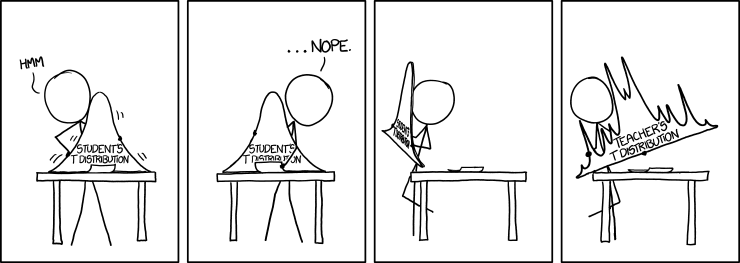
\includegraphics[width=\textwidth]{Graphiques/t_distribution}
				\end{minipage}
				&
				\begin{minipage}[l]{0.4\textwidth}
								Lorem ipsum dolor sit amet, consectetur adipiscing elit. Integer sapien mi, pretium ut consectetur a, congue eu odio. 
				\end{minipage}\\
			\end{tabular}

			
\code			
\begin{tabular}{cc}
	\begin{minipage}[l]{0.4\textwidth}
		Lorem ...
	\end{minipage}\vspace{0.3cm}
	&
	\begin{minipage}[l]{0.4\textwidth}
		Lorem ...
	\end{minipage}\vspace{0.3cm}\\
	\begin{minipage}[l]{0.4\textwidth}
		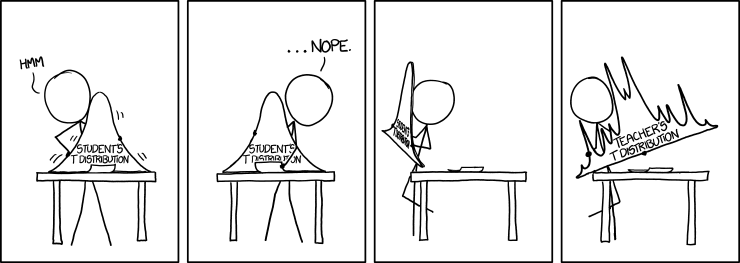
\includegraphics[width=\textwidth]
		{Graphiques/t_distribution}
	\end{minipage}
	&
	\begin{minipage}[l]{0.4\textwidth}
		Lorem ...
	\end{minipage}\\
\end{tabular}
\end{Verbatim}
		
\section{Babel\ldots}

  		\subsection{Un mot sur Babel}
  		
Pour �crire que M\up{me} s'est mari�e pour la 1\iere fois, c'est possible gr�ce � l'extension \textit{french} de Babel que vous trouverez dans le pr�ambule des documents qui vous sont fournis. 

\primo, \secundo, etc... et d'autres abbr�viations fran�aises sont possibles. Pour une revue de d�tail, voir l'ouvrage \textit{\latex par la pratique} de Christian \bsc{Rolland} qui donne aussi des clefs sur la typograhie fran�aise qui sont loin d'�tre toutes respect�es dans ce document.
  		
  		\code
Pour �crire que M\up{me} s'est mari�e pour la 1\ere fois
\primo, \secundo, ... 
Christian \bsc{Rolland}
		\end{Verbatim}

		



\section{Les unit�s dans \LaTeX}

  		\subsection{Les unit�s dans \LaTeX}
  		
		Les commandes impliquant des tailles permettent d'utiliser plusieurs des unit�s de taille. 
		
		Pour ces commandes, comme on l'a vu, on passe en argument � la commande la taille suivie de l'unit�.
		
		Les unit�s disponibles dans \latex sont pr�sent�es dans le tableau suivant. 




			% Table generated by Excel2LaTeX from sheet 'Feuil1'
			\begin{table}[h!]
			  \centering
			    \begin{tabular}{rcc}
			    \addlinespace
					Abbr�viaton & unit� & taille\\
					\toprule
			    {\bf Absolues} &       &  \\
			    \midrule
			    pt    & point & unit� de base \\
			    pc    & pica  & 1pc = 12 pt \\
			    in    & pouce & 1 in = 72,27 pt \\
			    cm    & centim�tre & 1 cm = 28,45 pt \\
			    mm    & millim�tre & 1 mm = 2,845 pt \\
			    {\bf Relatives} &       &  \\
			    \midrule
			    em    & cadratin & largeur de M dans la police courante \\
			    ex    & -     & hauteur de x dans la police courante \\
			    \end{tabular}
				\caption{Unit�s (tir� du FramaBook\latex)}
			  \label{tab:addlabel}
			\end{table}	



			Il y a dans \latex des dimensions qui sont pr�programm�es~:
			\begin{description}
				\item[textwidth] la largeur de la zone avec du texte sur la page
				\item[textheight] la hauteur de la zone avec du texte sur la page
				\item [marginparwidth] marge gauche...
				\item[etc.]				
			\end{description}
			
			On peut les utiliser simplement en appelant \textbackslash textwidth. Les op�rations de multiplications sont autoris�es~: par exemple 0.5\textbackslash textwidth correspond � la moiti� de la longueur de la ligne standard.
			
			Toutes les dimensions concernant les pages sont bien d�crites dans le \href{https://en.wikibooks.org/wiki/LaTeX/Page_Layout}{WikiBook \latex}.
			

\section{Les couleurs dans \LaTeX}

  		\subsection{Les couleurs dans \LaTeX}

			Comme on l'a vu plus haut, les couleurs n�cessitent le paquet \emph{color}. Ce paquet permet d'importer soixante huit couleurs de base~:
			
			Les principales~: 
	\begin{itemize}
		\item black
		\item white
		\item red
		\item green
		\item blue
		\item \dots
	\end{itemize}

		La liste compl�te se retrouve \href{http://en.wikibooks.org/wiki/LaTeX/Colors}{ici }


                
On les appelle par exemple avec la commande \emph{textcolor}
\code
\textcolor{red}{Mon texte en rouge}
\textcolor{green}{Mon texte en vert}
\end{Verbatim}
 
	

                
Mais on peut d�finir dans le pr�ambule son propre jeu de couleurs~: 
\code
\definecolor{nom}{mod�le}{taux} 
\end{Verbatim}

Mod�le d�finit trois possibilit�s~: gray, rgb ou cmyk.

	

  		\subsection{Les compteurs dans \LaTeX}
                
Pour gray, on donne un nombre entre 0 (noir) et 1(blanc).\\
Pour rgb~: 
\begin{enumerate}
\item on donne un nombre entre 0 (pas de rouge) et 1(rouge).
\item on donne un nombre entre 0 (pas de vert) et 1(vert).
\item on donne un nombre entre 0 (pas de bleu) et 1(blue).
\end{enumerate}
...
	
  		\subsection{Les couleurs dans \LaTeX}
                
Il suffit ensuite dans les commandes utilisant les couleurs
d'appeler sa couleur personnalis�e~:
\code
\definecolor{violet}{rgb}{0.5,0,0.5}
...
\textcolor{violet}{mon texte en violet}
\end{Verbatim}


                
\begin{table}[h!]
\begin{tabular}{lc}
Commande & Fonction\\
\hline
textcolor & coloriser du texte\\
colorbox & mettre un fond de couleur derri�re le texte\\
fcolorbox & mettre un fond de couleur avec une bordure\\
makebox & mettre un fond de couleur sur une largeur donn�e\\
pagecolor & changer le fond de la page\\
color & d�finir la couleur de tout le texte qui suit\\
\end{tabular}
\end{table}


\section{Les compteurs}
		
  		\subsection{Le principe des compteurs}
                
			Les compteurs sont des variables un peu particuli�res dans \latex. 
			
			Les compteurs sont d�finis et utilis�s par le compilateur et les macros. De nombreux compteurs existent~:
				\begin{description}
					\item[part, chapter, section, \ldots] ces nombreux compteurs identifient les pages et la num�rotation des �lements, \ldots
					\item[enumi, enumii, enumiii, enumiv] pour les listes num�rot�es par exemple.
					\item[equation] pour les num�ros d'�quation
					\item[\ldots]
				\end{description}
				
				Ils sont accessibles et modifiables.
				

  		\subsection{Liste partielle des compteurs}
                
\begin{center}
\begin{table}
	\begin{tabular}{llll}
		part & paragraph & figure & enumi\\
		chapter & subparagraph & table & enumii\\			
		section & page & footnote & enumiii\\
		subsection & equation & mpfootnote & enumiv\\
	\end{tabular}
\end{table}
\end{center}				



  		\subsection{Les fonctions \textbackslash the\ldots}
                
			Les fonctions \textbackslash the\ldots affichent le contenu du compteur. 
			
			Par exemple~: nous en sommes � la \thepage\up{�me} diapositive. 
			
			\code
Nous en sommes � la \thepage\up{�me} diapositive. 
\end{Verbatim}


      
      Ces compteurs peuvent �tre utilis�s pour g�n�rer des fonctions d'affichage personnels. La syntaxe fait appel � la d�finition de macros \latex.
      
\newcommand{\thediapo}{Diapo \arabic{page} sur \pageref{LastPage}}            
			Nous en sommes donc maintenant � la \thediapo.
      
\code 
\newcommand{\thediapo}%
{Diapo \arabic{page} sur \pageref{LastPage}}            
Nous en sommes donc maintenant � la \thediapo.
\end{Verbatim}
      

      
      Les compteurs par d�faut peuvent �tre modifi�s pour g�n�rer des fonctions d'affichage personnels. 
      
\renewcommand{\thepage}{Diapo \arabic{page} sur \pageref{LastPage}}            
Nous en sommes donc maintenant � la \thepage.
      
\code 
\renewcommand{\thepage}%
{Diapo \arabic{page} sur \pageref{LastPage}}            
Nous en sommes donc maintenant � la \thepage.
\end{Verbatim}

\renewcommand{\thepage}{\arabic{page}}            
      

      
      \latex des fonctions permettant de modifier le style de num�rotation...

\renewcommand{\thepage}{Diapo \Roman{page}}            
Nous en sommes donc maintenant � la \thepage.
      
\code 
\renewcommand{\thepage}%
{Diapo \Roman{page}}            
Nous en sommes donc maintenant � la \thepage.
\end{Verbatim}
      
\renewcommand{\thepage}{\arabic{page}}                  
      

      
      Outre ces possibilit�s, des compteurs propres � l'utilisateur peuvent �tre d�finis tr�s simplement~:
      
\code
\newcounter{cnt}
\setcounter{cnt}{7}
\arabic{cnt}
\addtocounter{cnt}{1}
\arabic{cnt}
\end{Verbatim}

\newcounter{cnt}
\setcounter{cnt}{7}
\arabic{cnt}
\addtocounter{cnt}{1}
\arabic{cnt}
    
    La d�finition de la valeur et l'incr�mentation est possible tant pour les \og~compteurs \latex~\fg que pour les compteurs de l'utilisateur.
    

		
      
      Enfin pour finir, les valeurs des compteurs peuvent �tre r�cup�r�s depuis d'autres compteurs\ldots
      
\code
\newcounter{cnt}
\setcounter{cnt}{\value{section}}
\arabic{cnt}
\end{Verbatim}

\setcounter{cnt}{\value{section}}
\arabic{cnt}
      
		



\documentclass{beamer}
\usetheme[compress]{Singapore}
\useoutertheme{miniframes}

% Pour les documents en fran�ais...
	\usepackage[latin1]{inputenc}
	\usepackage[french]{babel}    
	\usepackage[french]{varioref} 
	
% Math�matiques
	\usepackage{amsmath}
	
% A documenter	
	\usepackage{moreverb}
	\usepackage{lipsum}

% Pour ins�rer des graphiques	
	\usepackage{eso-pic,graphicx}	% Graphique simples    
	\usepackage{subfigure}			% Graphiques multiples
	\usepackage{xcolor}
	\usepackage{tikz}
	\usetikzlibrary{positioning}						
	
% Pour ins�rer des couleurs	
	\usepackage{color}

% Outil suppl�mentaire pour les tableaux
	\usepackage{multirow}
 	\usepackage{booktabs}
	\usepackage{longtable}
	\usepackage{colortbl}
	
% Rotation des objets et des pages
	\usepackage{rotating}
	\usepackage{lscape}

% Pour ins�rer du code source, LaTeX ou SAS par exemple.
	\usepackage{verbatim}
	\usepackage{fancyvrb}
	\usepackage{listings} 

% Pour ins�rer des hyperliens
	\usepackage{hyperref}

% American Psychological Association (for bibliographic references).
	\usepackage{apacite}
  
% Pour l'utilisation des macros
	\usepackage{xspace}

% Pour l'utilisation de notes en fin de document.
	\usepackage{endnotes}

% Rotation
	\usepackage{rotating}

% Pour les t�ches de caf�
	\usepackage{coffee}

% Symboles suppl�mentaires
	\usepackage{bbding}
	\usepackage{pifont}

% Pour les listes num�rot�es
	\usepackage{enumerate}

% Pour la derni�re page
	\usepackage{lastpage}

% Pour Highlight d'Andre Simon
\usepackage{alltt}

% pour les symboles
\usepackage{keystroke}
%\usepackage{feyn}
\usepackage{bbding}
\usepackage{phonetic}

% Pour ins�rer des dessins de Linux
\newcommand{\LinuxA}{
\includegraphics[height=0.5cm]{Graphiques/linux.png}}
\newcommand{\LinuxB}{
\includegraphics[height=0.5cm]{Graphiques/linux.png}\xspace}

% Macro pour les petits dessins pour les diff�rents OS.
\newcommand{\Windows}{\emph{Windows}\xspace}
\newcommand{\Mac}{\emph{Mac OS X}\xspace}
\newcommand{\Linux}{\emph{Linux}\xspace}
\newcommand{\MikTeX}{MiK\tex\xspace}

% Des raccourcis pour les commandes \LaTeX, \TeX, ...
\newcommand{\latex}{\LaTeX\xspace}
\newcommand{\latexe}{\LaTeXe\xspace}
\newcommand{\tex}{\TeX\xspace}

% Commande pour le mode Verbatim
\newcommand{\code}{\vspace{0.2cm}\begin{Verbatim}[frame=single,label=Code,fontsize=\small]}
\newcommand{\tinycode}{\vspace{0.2cm}\begin{Verbatim}[frame=single,label=Code,fontsize=\tiny]}

% From Framabook (www.framasoft.net)
\newcommand{\latexcom}[1]{{\mdseries\ttfamily\upshape\symbol{92}#1}}
\newcommand{\indexcom}[1]{%
  \index{#1@\protect\texttt{\symbol{92}#1}}}
\newcommand{\ltxcom}[1]{%
  \latexcom{#1}\indexcom{#1}}  

\newcommand{\hlstd}[1]{\textcolor[rgb]{0,0,0}{#1}}
\newcommand{\hlnum}[1]{\textcolor[rgb]{0.5,0,0.5}{\bf{#1}}}
\newcommand{\hlesc}[1]{\textcolor[rgb]{1,0,1}{\bf{#1}}}
\newcommand{\hlstr}[1]{\textcolor[rgb]{0.65,0.52,0}{#1}}
\newcommand{\hlpps}[1]{\textcolor[rgb]{0,0,1}{#1}}
\newcommand{\hlslc}[1]{\textcolor[rgb]{0.95,0.47,0}{#1}}
\newcommand{\hlcom}[1]{\textcolor[rgb]{1,0.5,0}{#1}}
\newcommand{\hlppc}[1]{\textcolor[rgb]{0,0.5,0.75}{\bf{#1}}}
\newcommand{\hlopt}[1]{\textcolor[rgb]{1,0,0.5}{\bf{#1}}}
\newcommand{\hlipl}[1]{\textcolor[rgb]{0.62,0.36,1}{#1}}
\newcommand{\hllin}[1]{\textcolor[rgb]{0.19,0.19,0.19}{#1}}
\newcommand{\hlkwa}[1]{\textcolor[rgb]{0.73,0.47,0.47}{\bf{#1}}}
\newcommand{\hlkwb}[1]{\textcolor[rgb]{0.5,0.5,0.75}{\bf{#1}}}
\newcommand{\hlkwc}[1]{\textcolor[rgb]{0,0.5,0.75}{#1}}
\newcommand{\hlkwd}[1]{\textcolor[rgb]{0,0.27,0.4}{#1}}


\newcommand{\yslant}{0.5}
\newcommand{\xslant}{-0.6}
		 
% Titre		 
\title{Introduction � \LaTeX}
\author{Pascal Bessonneau}
\date{05/2016}




	
	














 				\subtitle{\'Ecrire des math�matiques}

\begin{document}

  \begin{frame}
  \titlepage
  \end{frame}

  \begin{frame}<beamer>
    \frametitle{Plan}
    \tableofcontents
  \end{frame}

\section{Les math�matiques}

		\begin{frame}[containsverbatim]
  		\frametitle{Le langage � l'int�rieur des environnements}

			Les lettres et les chiffres sont conserv�s. Les espaces sont supprim�s. Les deux symboles incontournables sont~:
	
\code			
X_{ijk} et e^{ax+b}
\end{Verbatim}
			
			Le soulign�, \_ ,  permet de mettre i en indice de X. Le \textasciicircum permet de mettre en exposant tout ce qui est entre accolades. Les accolades sont optionnelles s'il n'y a pas d'ambiguit� dans la syntaxe~: 
			
			\code			
			X_i et e^a
			\end{Verbatim}

  	\end{frame}			
			
		\begin{frame}[containsverbatim]
  		\frametitle{Le langage � l'int�rieur des environnements}
			
			\code			
			\frac{a}{b}
			\end{Verbatim}
			
			qui donne la division $\frac{a}{b}$.
			
  	\end{frame}

		\begin{frame}[containsverbatim]
  		\frametitle{Le langage � l'int�rieur des environnements}

			\begin{displaymath}
			\sqrt{\frac{1+\sqrt[3]{3x+1}}{3x+\frac{1-x}{1+x}}}
			\end{displaymath}

\code			
\sqrt{\frac{1+\sqrt[3]{3x+1}}{3x+\frac{1-x}{1+x}}}
\end{Verbatim}

  	\end{frame}

		\begin{frame}[containsverbatim]
  		\frametitle{Et les int�grales et sommes ?}
  		
			\begin{displaymath}
				\ln(x)=\int_{1}^{x}\frac{1}{t}\mathrm{d}t
			\end{displaymath}

			\code			
\ln(x)=\int_{1}^{x}\frac{1}{t}\mathrm{d}t
			\end{Verbatim}
		
  	\end{frame}

		\begin{frame}[containsverbatim]
  		\frametitle{Et les int�grales et sommes ?}
  		
			\begin{displaymath}
				\sum_{i=0}^{n}q^i=\frac{1-q^{n+1}}{1-q}
			\end{displaymath}

			\code			
\sum_{i=0}^{n}q^i=\frac{1-q^{n+1}}{1-q}
			\end{Verbatim}
		
  	\end{frame}


		\begin{frame}[containsverbatim]
  		\frametitle{Et les int�grales et sommes ?}
  		
			\begin{displaymath}
\int\limits_{-\infty}^{\infty}x^2=\left[\frac{1}{3}x^3\right]_{-\infty}^{\infty}
			\end{displaymath}

\code			
\int\limits_{-\infty}^{\infty}x^2
=\left[x^2\right]_{-\infty}^{\infty}
\end{Verbatim}
		
  	\end{frame}


		\begin{frame}[containsverbatim]
  		\frametitle{Une racine n-�me}
  		
			\begin{displaymath}
				\sqrt[3]{\frac{3x}{2y-3}}
			\end{displaymath}

			\code			
\sqrt[3]{\frac{3x}{2y-3}}
			\end{Verbatim}
		
  	\end{frame}

\section{Les diff�rents environnements}

		\begin{frame}[containsverbatim]
  		\frametitle{En ligne}
  		
  		Les commandes pour faire des math�matiques en ligne, c'est-�-dire sans cr�er de paragraphe, sont les suivantess : \textdollar, \textbackslash begin\{math\}. Pour fermer ces environnements, on utilise respectivement \textdollar, \textbackslash end\{math\}. 
  		
  		Par exemple : $y = ax + b$ s'�crit tout simplement...
  		
			\code
Par exemple : $y = ax + b$ s'�crit tout simplement...
			\end{Verbatim}

  	\end{frame}

		\begin{frame}[containsverbatim]
  		\frametitle{En ligne}
  		
  		Pour ins�rer la formule du mod�le de Rasch � l'int�rieur d'une phrase, un seul \textdollar\ est suffisant~: $P(X_{i}=1)=\frac{1}{1+e^{(\theta_{i}-\beta_{i})}}$
  		
			\code
$P(X_{i}=1)=\frac{1}{1+e^{(\theta_{i}-\beta_{i})}}$
			\end{Verbatim}
			
  	\end{frame}

		\begin{frame}[containsverbatim]
  		\frametitle{Mise en �vidence}
  		
  		Les commandes pour faire des maths en cr�ant un paragraphe sous \latex sont les suivantes~: \textdollar\textdollar, \textbackslash begin\{displaymath\}. 
  		Pour fermer ces environnements, on utilise respectivement \textdollar\textdollar, \textbackslash end\{displaymath\}. 

			Par exemple : 
			$$y = ax + b$$
			s'�crit tout simplement...
  		
			\code
Par exemple : 
$$y = ax + b$$
s'�crit tout simplement...
			\end{Verbatim}
  					
  	\end{frame}


		\begin{frame}[containsverbatim]
  		\frametitle{Mise en �vidence}
					
			Il existe une diff�rence non n�gligeable entre les deux �critures. Dans le cas du \$ simple, les formules doivent tenir sur la hauteur d'une ligne de texte. Ceci a pour cons�quence que les indices de certains op�rateurs comme les sommes par exemple ne sont pas l� o� l'on souhaiterait les voir~:
			
			\vspace{0.5cm}
			bla bla bla $\sum_{i=0}^{k}$ bla bla bla 
			\vspace{0.5cm}
			
			Par contre avec \$\$ dans ce cas, \latex n'est plus contraint pas la hauteur de la ligne et l'aspect est plus agr�able � l'oeil.
			
			$$\sum_{i=0}^{k}$$
  		  					
  	\end{frame}


		\begin{frame}[containsverbatim]
  		\frametitle{Pour une �quation}
  		
  		La commande pour �crire des �quations est la suivante : \textbackslash begin\{equation\}. 
  		Pour fermer l'environnement on utilise \textbackslash end\{equation\}. 

			Par exemple : 
			\begin{equation}y = ax + b\end{equation}
			s'�crit tout simplement...
  		
			\code
Par exemple : 
\begin{equation}y = ax + b\end{equation}
s'�crit tout simplement...
			\end{Verbatim}
  					
  	\end{frame}

		\begin{frame}[containsverbatim]
  		\frametitle{Pour une s�rie d'�quations}
  		
  		La commande pour �crire une s�rie d'�quations est la suivante : \textbackslash begin\{eqnarray\}. 
  		Pour fermer cet environnement, on utilise \textbackslash end\{eqnarray\}. 

			Par exemple : 
			\begin{eqnarray}
			y & = & ax + b\\
			a & = & \frac{y-b}{a}\label{myeq}\\
			  & et &\nonumber\\
			b & = & y - ax
			\end{eqnarray}
			s'�crit tout simplement...
  		
			Et vous pouvez faire r�f�rence � l'�quation \eqref{myeq}.
			
  	\end{frame}


		\begin{frame}[containsverbatim]
  		\frametitle{Pour une s�rie d'�quations}
  		
  		Le texte correspondant est~:
\code
\begin{eqnarray}
y & = & ax + b\\
a & = & \frac{y-b}{a}\label{myeq}\\
	& et &\nonumber\\
b & = & y - ax
\end{eqnarray}

Et vous pouvez faire r�f�rence � l'�quation \eqref{myeq}.
\end{Verbatim}
			
  	\end{frame}


		\begin{frame}[containsverbatim]
  		\frametitle{Pour une s�rie d'�quations}
  		
			\code
Par exemple : 
\begin{eqnarray}
	y & = & ax + b\\
	a & = & \frac{y-b}{a}\\
  	& et &\nonumber\\
	b & = & y - ax\\
\end{eqnarray}
s'�crit tout simplement...
			\end{Verbatim}

  					
  	\end{frame}

		\begin{frame}[containsverbatim]
  		\frametitle{Pour une s�rie d'�quations}
  		
			Comme son nom l'indique, \emph{eqnarray} permet d'aligner des morceaux des �quations.
			
			Dans l'exemple pr�c�dent, on veut que la partie gauche, le signe = et enfin la partie droite soient align�s. Pour se faire, on utilise la m�me terminologie que pour les tableaux vus pr�c�demment avec \& et \textbackslash\textbackslash.
  					
  	\end{frame}

		\begin{frame}[containsverbatim]
  		\frametitle{Supprimer ou modifier la num�rotation}

			Il faut utiliser l'* qui modifie le comportement des fonctions comme pour les titre de parties ou sections.
			
			Soit~:
\code			
\begin{equation*}			
ou
\begin{eqnarray*}			
\end{Verbatim}
			
			Enfin, pour ne pas num�roter une ligne parmi l'ensemble, il faut placer la commande \textbackslash nonumber � la fin.
  					
  	\end{frame}

		\begin{frame}[containsverbatim]
  		\frametitle{Syst�me d'�quations}
  		
			Dans un syst�me d'�quations, il est n�cessaire d'ajouter une accolade~:
			
			\begin{displaymath}
			\left\{
				\begin{array}{lll}
				x & = & 4a^2 + 5b -c \\
				y & = & 7a^2 + b - 3c\\
				z & = & b + 4c\\
				\end{array}
				\right.
			\end{displaymath}  					
			
  	\end{frame}

		\begin{frame}[containsverbatim]
  		\frametitle{Syst�me d'�quations}
  		
\code
\begin{displaymath}
	\left\{
		\begin{array}{lll}
			x & = & 4a^2 + 5b -c \\
			y & = & 7a^2 + b - 3c\\
			z & = & b + 4c	
		\end{array}
	\right.
\end{displaymath}  					
\end{Verbatim}

		Il est � noter ici que l'on peut ins�rer un tableau � l'int�rieur et utiliser la m�me syntaxe que pour \emph{eqnarray}.
			
  	\end{frame}

		\begin{frame}[containsverbatim]
  		\frametitle{Syst�me d'�quations}

			Enfin ici, on a une accolade � gauche mais rien � droite. Donc la syntaxe est~:
			\code
			\left\{
			...
			\right.
			\end{Verbatim}

			Le point indique qu'aucun symbole n'est utilis� pour fermer la partie droite. 
  		
  	\end{frame}

		\begin{frame}[containsverbatim]
  		\frametitle{Pour un ensemble plus complexe}
  		  		
			Si on combine deux tableaux~:

			$$
			\begin{array}{lll}
			A & = & \left\{
				\begin{array}{lll}
				x & = & 4a^2 + 5b -c \\
				y & = & 7a^2 + b - 3c\\
				z & = & b + 4c	
				\end{array}
				\right.\\
			B & = &\left\{
				\begin{array}{lll}
				x & = & 6a^2 + 3b -c \\
				y & = & 2a^2 + 4b - 7c\\
				z & = & 2b + c	
				\end{array}
				\right.\\
			\end{array}  					
		$$
  	\end{frame}

		\begin{frame}[containsverbatim]
  		\frametitle{Pour un ensemble plus complexe}
  		
\code
$$
\begin{array}{lll}
A & = & \left\{
	\begin{array}{lll}
	x & = & 4a^2 + 5b -c \\
	y & = & 7a^2 + b - 3c\\
	z & = & b + 4c	
	\end{array}
	\right.\\
B & = &\left\{
	\begin{array}{lll}
	x & = & 6a^2 + 3b -c \\
	y & = & 2a^2 + 4b - 7c\\
	z & = & 2b + c	
	\end{array}
	\right.\\
\end{array}  					
$$
\end{Verbatim}

  	\end{frame}

		\begin{frame}[containsverbatim]
  		\frametitle{Note sur les parenth�ses et accolades....}

			\code
\left(
	\begin{array}{ccc}
		1 & 0 & 0\\
		0 & 1 & 0\\
		0 & 0 & 1\\
	\end{array}
\right)
			\end{Verbatim}

			Ici on veut repr�senter la matrice identit�, il faut un symbole des deux cot�s...
  		
  	\end{frame}
  	
		\begin{frame}[containsverbatim]
  		\frametitle{Note sur les parenth�ses et accolades....}

			$$
			\left[
			\begin{array}{ccc}
			1 & 0 & 0\\
			0 & 1 & 0\\
			0 & 0 & 1\\
			\end{array}
			\right]
			$$
			
			On notera que comme $\{$ a un sens pour le langage, on le pr�c�de d'un \textbackslash. Par contre ce n'est pas le cas pour $($ et $[$.
  		
  	\end{frame}

\section{Les matrices}

		\begin{frame}[containsverbatim]
  		\frametitle{Un environnement pour les matrices}

\begin{displaymath}
\begin{pmatrix} 
D_1t				&-a_{12}t_2		&	\dots	&-a_{1n}t_n\\
-a_{21}t_1	&D_2t					&\dots	&-a_{2n}t_n\\
\hdotsfor[2]{4}\\
-a_{n1}t_1	&-a_{n2}t_2		&\dots	&D_nt
\end{pmatrix}
\end{displaymath}

  	\end{frame}

		\begin{frame}[containsverbatim]
  		\frametitle{Un environnement pour les matrices}
  	
\code
\begin{pmatrix} 
	D_1t        &-a_{12}t_2   &\dots &-a_{1n}t_n\\
	-a_{21}t_1  &D_2t         &\dots  &-a_{2n}t_n\\
	\hdotsfor[2]{4}\\
	-a_{n1}t_1  &-a_{n2}t_2   &\dots  &D_nt
\end{pmatrix}
\end{Verbatim}

			En fait �a marche presque comme un tableau avec des \& et \textbackslash \textbackslash.

  	\end{frame}		

\section{L'insertion de texte}

	\begin{frame}[containsverbatim]
  		\frametitle{Le texte simple}

		Comme on l'a vu, le texte est interpr�t� diff�remment, en italique.
		
		Mais dans des formules on peut vouloir rajouter du texte avec une police normal.
		
		Dans ce cas on utilise la commande \textbackslash text. Dans les \emph{text} les espaces sont conserv�s.
		
		$$\text{Soit } x \text{ et } y$$
		
		s'�crit...
		
		\code
$$\text{Soit } x \text{ et } y$$
		\end{Verbatim}

	\end{frame}

\section{Les accents typographiques et math�matiques}

	\begin{frame}[containsverbatim]
  		\frametitle{Les accents}

			Les accents dans le mode math�matique ne sont pas g�r�s par le package babel comme dans le texte normal.\\
			
			\vspace{0.1cm}
			Il faut donc les appeler avec une syntaxe particuli�re~:~$\acute{E}nergie=masse*c\acute{e}l\acute{e}rit\acute{e}^2$ soit~:
			\code
$\acute{E}nergie=masse*c\acute{e}l\acute{e}rit\acute{e}^2$
			\end{Verbatim}
			
			\end{frame}
			
	\begin{frame}[containsverbatim]
  		\frametitle{Les accents texte et math�matiques}
			
			Le m�me concept est � appliquer pour les accents au-dessus d'un vecteur, d'une moyenne,...
			
\begin{table}[h!]
\begin{center}

  \begin{tabular}{lc@{\quad}lc@{\quad}lc}
    \ltxcom{hat}\verb+{x}+  &$\hat{x}$  & \ltxcom{check}\verb+{x}+&$\check{x}$&
    \ltxcom{breve}\verb+{x}+&$\breve{x}$\\
    \ltxcom{acute}\verb+{x}+&$\acute{x}$& \ltxcom{grave}\verb+{x}+&$\grave{x}$&
    \ltxcom{tilde}\verb+{x}+&$\tilde{x}$\\ 
    \ltxcom{bar}\verb+{x}+  &$\bar{x}$  & \ltxcom{dot}\verb+{x}+&$\dot{x}$&
    \ltxcom{ddot}\verb+{x}+ &$\ddot{x}$\\  
  \end{tabular}
\caption{Les accents en mode math�matique (FramaBook \LaTeX)}
\end{center}
\end{table}			

	\end{frame}
	
	\begin{frame}[containsverbatim]
  		\frametitle{Les accents math�matiques...}
			
			Pour les fl�ches des calculs vectoriels, il y a, selon la longueur la commande \emph{vec} pour une lettre sinon la commande \emph{overrightarrow}.\\
			
			\vspace{0.1cm}
			$ \vec{a} \mbox{ et } \overrightarrow{AB} $ s'�crit~:
						
			\code
$ \vec{a} \mbox{ et } \overrightarrow{AB} $
			\end{Verbatim}

	\end{frame}			

	\begin{frame}[containsverbatim]
  		\frametitle{Les accents math�matiques...}
			
	Toute une liste de symboles math�matiques du m�me type que \emph{overrightarrow} est utilisable. Je vous invite � consulter la liste des caract�res sp�ciaux d�j� \href{ftp://tug.ctan.org/pub/tex-archive/info/symbols/comprehensive/symbols-letter.pdf}{cit�e}.

	\end{frame}

	\begin{frame}[containsverbatim]
  		\frametitle{Les accents math�matiques...}
			
Par exemple, il suffit d'appeler la commande~:

			\code
$$\underbrace{monequation}$$
			\end{Verbatim}
			
		$$\underbrace{monequation}$$
				

	\end{frame}

\section{Le style de police et les espaces}

	\begin{frame}[containsverbatim]
  		\frametitle{Les fonctions usuelles}
			
	Nous avons pu noter que le texte est mis en italique dans le mode math�matique. Mais ce n'est pas le comportement que l'on attend pour les fonctions usuelles telles que sin, cos, ln,... qui ne doivent pas �tre en italique...
	
			En fait il suffit de faire pr�c�der le nom de la fonction par un \textbackslash, en effet la plupart des fonctions usuelles sont reconnues par \LaTeX~: $\sin \; \cos \; \ln \; ...$.
			
			\code
$\sin \; \cos \; \ln \; ...$
			\end{Verbatim}
		 
	\end{frame}

	\begin{frame}[containsverbatim]
  		\frametitle{Les polices}
			
	Pour changer et avoir la police des ensembles les commandes sont les suivantes~:
	
	\vspace{0.2cm}
\begin{table}[h!]
	\begin{center}

  \begin{tabular}{lc}
    \verb+Soit $+\ltxcom{mathit}\verb+{A\in\Phi}$+ &    Soit $\mathit{A\in\Phi}$ \\
    \verb+Soit $+\ltxcom{mathrm}\verb+{A\in\Phi}$+ &    Soit $\mathrm{A\in\Phi}$ \\
    \verb+Soit $+\ltxcom{mathbf}\verb+{A\in\Phi}$+ &    Soit $\mathbf{A\in\Phi}$ \\
    \verb+Soit $+\ltxcom{mathsf}\verb+{A\in\Phi}$+ &    Soit $\mathsf{A\in\Phi}$ \\
    \verb+Soit $+\ltxcom{mathtt}\verb+{A\in\Phi}$+ &    Soit $\mathtt{A\in\Phi}$ \\
    \verb+Soit $+\ltxcom{mathcal}\verb+{A}\in\Phi$+&    Soit $\mathcal{A}\in\Phi$ \\
  \end{tabular}
\caption{Les polices en mode math�matique (FramaBook \LaTeX)}
  \end{center}
  \end{table}
  
	\end{frame}

	\begin{frame}[containsverbatim]
  		\frametitle{Les espaces}
			
	Pour ins�rer des espaces dans des �quations il suffit d'utiliser les commandes suivantes~:
	
	\begin{table}[h!]
  \begin{center}
    {\addtolength{\extrarowheight}{5pt}
    \begin{tabular}{|ll|ll|ll|ll|}
      \hline
      \verb+\!+ & $\Box\!\Box$ &
      \emph{(rien)} & $\Box\Box$ &
      \verb+\,+ & $\Box\,\Box$ &
      \verb+\:+ & $\Box\:\Box$ \\
      \hline
      \verb+\;+ & $\Box\;\Box$ &
      \verb*+\ + & $\Box\ \Box$ &
      \ltxcom{quad} & $\Box\quad\Box$ &
      \ltxcom{qquad} & $\Box\qquad\Box$ \\
      \hline
    \end{tabular}}
\caption{Les espaces en mode math�matique (FramaBook \LaTeX)}
  \end{center}
 \end{table}

	\end{frame}


\section{AMSMath}
 
		\begin{frame}[containsverbatim]
  		\frametitle{AMSMath}

			Le paquet \emph{amsmath} permet d'�tendre les capacit�s de \latex en mati�re de mise en page des math�matiques.
  		
				\begin{align}
(a+b)^2 & = (a+b)(a+b)\\
				& = a^2+b^2+2ab
				\end{align}

			\code			
\begin{align}
(a+b)^2	& = (a+b)(a+b)\\
	& = a^2+b^2+2ab
\end{align}
			\end{Verbatim}
		
  	\end{frame}

		\begin{frame}[containsverbatim]
  		\frametitle{Un petit syst�me d'�quation ?}

			Pour cela, on peut passer par le paquet \emph{amsmath}~:

\begin{displaymath}
P_{r-j}=\begin{cases}
0& \text{if $r-j$ is odd},\\
r!\,(-1)^{(r-j)/2}& \text{if $r-j$ is even}.
\end{cases}
\end{displaymath}

			\code			
P_{r-j}=\begin{cases}
	0	& \text{if $r-j$ is odd},\\
	r!\,(-1)^{(r-j)/2} & \text{if $r-j$ is even}.
\end{cases}
			\end{Verbatim}
		
  	\end{frame}
				
\end{document}


\documentclass{beamer}
\usetheme[compress]{Singapore}
\useoutertheme{miniframes}

% Pour les documents en fran�ais...
	\usepackage[latin1]{inputenc}
	\usepackage[french]{babel}    
	\usepackage[french]{varioref} 
	
% Math�matiques
	\usepackage{amsmath}
	
% A documenter	
	\usepackage{moreverb}
	\usepackage{lipsum}

% Pour ins�rer des graphiques	
	\usepackage{eso-pic,graphicx}	% Graphique simples    
	\usepackage{subfigure}			% Graphiques multiples
	\usepackage{xcolor}
	\usepackage{tikz}
	\usetikzlibrary{positioning}						
	
% Pour ins�rer des couleurs	
	\usepackage{color}

% Outil suppl�mentaire pour les tableaux
	\usepackage{multirow}
 	\usepackage{booktabs}
	\usepackage{longtable}
	\usepackage{colortbl}
	
% Rotation des objets et des pages
	\usepackage{rotating}
	\usepackage{lscape}

% Pour ins�rer du code source, LaTeX ou SAS par exemple.
	\usepackage{verbatim}
	\usepackage{fancyvrb}
	\usepackage{listings} 

% Pour ins�rer des hyperliens
	\usepackage{hyperref}

% American Psychological Association (for bibliographic references).
	\usepackage{apacite}
  
% Pour l'utilisation des macros
	\usepackage{xspace}

% Pour l'utilisation de notes en fin de document.
	\usepackage{endnotes}

% Rotation
	\usepackage{rotating}

% Pour les t�ches de caf�
	\usepackage{coffee}

% Symboles suppl�mentaires
	\usepackage{bbding}
	\usepackage{pifont}

% Pour les listes num�rot�es
	\usepackage{enumerate}

% Pour la derni�re page
	\usepackage{lastpage}

% Pour Highlight d'Andre Simon
\usepackage{alltt}

% pour les symboles
\usepackage{keystroke}
%\usepackage{feyn}
\usepackage{bbding}
\usepackage{phonetic}

% Pour ins�rer des dessins de Linux
\newcommand{\LinuxA}{
\includegraphics[height=0.5cm]{Graphiques/linux.png}}
\newcommand{\LinuxB}{
\includegraphics[height=0.5cm]{Graphiques/linux.png}\xspace}

% Macro pour les petits dessins pour les diff�rents OS.
\newcommand{\Windows}{\emph{Windows}\xspace}
\newcommand{\Mac}{\emph{Mac OS X}\xspace}
\newcommand{\Linux}{\emph{Linux}\xspace}
\newcommand{\MikTeX}{MiK\tex\xspace}

% Des raccourcis pour les commandes \LaTeX, \TeX, ...
\newcommand{\latex}{\LaTeX\xspace}
\newcommand{\latexe}{\LaTeXe\xspace}
\newcommand{\tex}{\TeX\xspace}

% Commande pour le mode Verbatim
\newcommand{\code}{\vspace{0.2cm}\begin{Verbatim}[frame=single,label=Code,fontsize=\small]}
\newcommand{\tinycode}{\vspace{0.2cm}\begin{Verbatim}[frame=single,label=Code,fontsize=\tiny]}

% From Framabook (www.framasoft.net)
\newcommand{\latexcom}[1]{{\mdseries\ttfamily\upshape\symbol{92}#1}}
\newcommand{\indexcom}[1]{%
  \index{#1@\protect\texttt{\symbol{92}#1}}}
\newcommand{\ltxcom}[1]{%
  \latexcom{#1}\indexcom{#1}}  

\newcommand{\hlstd}[1]{\textcolor[rgb]{0,0,0}{#1}}
\newcommand{\hlnum}[1]{\textcolor[rgb]{0.5,0,0.5}{\bf{#1}}}
\newcommand{\hlesc}[1]{\textcolor[rgb]{1,0,1}{\bf{#1}}}
\newcommand{\hlstr}[1]{\textcolor[rgb]{0.65,0.52,0}{#1}}
\newcommand{\hlpps}[1]{\textcolor[rgb]{0,0,1}{#1}}
\newcommand{\hlslc}[1]{\textcolor[rgb]{0.95,0.47,0}{#1}}
\newcommand{\hlcom}[1]{\textcolor[rgb]{1,0.5,0}{#1}}
\newcommand{\hlppc}[1]{\textcolor[rgb]{0,0.5,0.75}{\bf{#1}}}
\newcommand{\hlopt}[1]{\textcolor[rgb]{1,0,0.5}{\bf{#1}}}
\newcommand{\hlipl}[1]{\textcolor[rgb]{0.62,0.36,1}{#1}}
\newcommand{\hllin}[1]{\textcolor[rgb]{0.19,0.19,0.19}{#1}}
\newcommand{\hlkwa}[1]{\textcolor[rgb]{0.73,0.47,0.47}{\bf{#1}}}
\newcommand{\hlkwb}[1]{\textcolor[rgb]{0.5,0.5,0.75}{\bf{#1}}}
\newcommand{\hlkwc}[1]{\textcolor[rgb]{0,0.5,0.75}{#1}}
\newcommand{\hlkwd}[1]{\textcolor[rgb]{0,0.27,0.4}{#1}}


\newcommand{\yslant}{0.5}
\newcommand{\xslant}{-0.6}
		 
% Titre		 
\title{Introduction � \LaTeX}
\author{Pascal Bessonneau}
\date{05/2016}




	
	














 				\subtitle{R�f�rences et Bib\TeX}

\begin{document}

  \begin{frame}
  \titlepage
  \end{frame}

  \begin{frame}<beamer>
    \frametitle{Plan}
    \tableofcontents
  \end{frame}	


\section{Faire r�f�rence � des �l�ments du document}

		\begin{frame}[containsverbatim]
  		\frametitle{Remarques sur la compilation}
  		
Lors de la compilation \latex ne cr�e pas par d�faut tous les fichiers n�cessaires � tous les types de r�f�rence. Notamment pour les r�f�rences bibliographiques, il faudra appeler des logiciels suppl�mentaires comme \textit{makeIndex} et \textit{bibtex}. 

Ces "options" de compilation sont propos�es par tous les logiciels d�di�s � \latex mais il faudra penser � ces commandes par exemple si on compile en ligne de commande.

\end{frame}

		\begin{frame}[containsverbatim]
  		\frametitle{Figures ou tableaux}
  		
Au moment de la cr�ation du tableau ou de la figure, on a utilis� la commande~:
 		
\tinycode
\label{Tableau_Niveaux}
\end{Verbatim}

Il suffit alors d'appeler \emph{ref} avec le nom de l'�tiquette pour
avoir le num�ro de l'�lement et \emph{pageref} pour avoir le num�ro de page.

\tinycode
Le Tableau \ref{Tableau_Niveaux}
page \pageref{Tableau_Niveaux} le tableau...
\end{Verbatim}

  	\end{frame}

		\begin{frame}[containsverbatim]
  		\frametitle{Faire r�f�rence � une section}
  		
Au moment de la cr�ation de l'appel de la section, il suffit d'ajouter
une commande \emph{label}~:
 		
\tinycode
\section{Ma section}\label{MaSection}
...
Vu en section \ref{MaSection}
\end{Verbatim}

  	\end{frame}

\section{Cr�er le fichier de r�f�rence bibliographiques}

		\begin{frame}[containsverbatim]
  		\frametitle{Un fichier Bib\TeX}
  		
  		Un fichier Bib\TeX est un fichier texte de ce type :
  		
\tinycode
@BOOK{Holland2007,
	title={Linking and aligning scores and scales},
	publisher = {Springer},
	year=2007,
	author={{N.J.} Dorans and M. Pommerich and {P.W.} Holland}
}
\end{Verbatim}

  	\end{frame}
  	
  			\begin{frame}[containsverbatim]
  		\frametitle{L'entr�e d�compos�e...}

			Apr�s le \at, on indique le type de support. Puis on donne un nom unique qui sera utilis� pour appeler la r�f�rence.  		
			
\tinycode
@BOOK{Holland2007,
\end{Verbatim}
		
		Ensuite on entre le contenu de chaque mot-clef, s�par� par des virgules, avec des accolades.

\tinycode
	title={Linking and aligning scores and scales},
	publisher = {Springer},
	year=2007,
	author={{N.J.} Dorans and M. Pommerich and {P.W.} Holland}
}
\end{Verbatim}  		
  	
  	\end{frame}	

\begin{frame}[containsverbatim]
  		\frametitle{L'entr�e d�compos�e...}

		Contrairement � \latex qui permet le support des caract�res accentu�s, dans bibtex il est plus simple d'utiliser les commandes \latex pour cr�er les caract�res accentu�es.
		
		C'est-�-dire \textbackslash', \textbackslash`, \dots
		
		Attention �galement pour le n� du volume, qui s'�crira \textbackslash textordmasculine.
  	
\end{frame}
  	
  	\begin{frame}[containsverbatim]
  		\frametitle{L'entr�e d�compos�e...}

		Pour les auteurs, je vous conseille de copier le style d'entr�e pr�cis� car il correspond au style de l'American Psychology Association (APA).
		
\tinycode
	author={{N.J.} Dorans and M. Pommerich and {P.W.} Holland}
\end{Verbatim}  		
		
		Le \emph{and} est reconnu par Bib\tex et permet de pr�senter correctement les noms et les abbr�viations pour les noms d'auteurs.
  	
\end{frame}


  	\begin{frame}[containsverbatim]
  		\frametitle{Le r�le des accolades}

		Les accolades permettent de d�limiter clairement les champs. Cette syntaxe est utilis�e par d�faut par JabRef.
		
		Les accolades permettent �galement de pr�venir des ambigu�t�s dans les noms des auteurs. Ici elles ont �t� utilis�es pour grouper les initiales des pr�noms mais sont �galement utiles pour les noms de famille compos�s.
		
\tinycode
	author = {M. {von Davier} and C. H. Carstensen}
\end{Verbatim}  		
 	
\end{frame}

		\begin{frame}[containsverbatim]
  		\frametitle{Un fichier Bib\TeX}

			Il existe plusieurs types de documents :
			
			\begin{description}
				\item[book] un livre
				\item[article] un article de p�riodique
				\item[conference] un intervention lors d'une conf�rence
				\item[inbook] une partie d'un livre.
				\item [etc.]
			\end{description}
			
			Chaque type a des champs optionnels et des champs requis.
			
  	\end{frame}
			
		\begin{frame}[containsverbatim]
  		\frametitle{Les champs obligatoires (article)}

			Pour un article par exemple les champs requis sont :
			\begin{itemize}
				\item author
				\item title
				\item journal
				\item year
			\end{itemize}
				
			\end{frame}

		\begin{frame}[containsverbatim]
  		\frametitle{Les champs facultatifs (article)}
			
			Les champs optionnels sont :
			
			\begin{itemize}
				\item volume
				\item number
				\item pages
				\item month
				\item note
				\item key
			\end{itemize}
			
  	\end{frame}

\section{Appeler une r�f�rence bibliographique}

  	\begin{frame}[containsverbatim]
  		\frametitle{Comment citer ?}
			
			Un autre type Pour citer l'ouvrage, il suffit alors d'utiliser la commande~: 
			
\tinycode
\cite{Holland2007}
ou
\citeA{Holland2007}
\end{Verbatim}		

		\end{frame}

  	\begin{frame}[containsverbatim]
  		\frametitle{Comment citer ?}
			
\begin{description} 
	\item[\textbackslash cite] Les �tudes psychom�triques, enrichies par les questionnaires sur les pratiques informatiques, pourront probablement apporter des informations sur la perception et les difficult�s propres � chaque type de t�ches et/ou items. Nous pensons par exemple � l'analyse avec des mod�les de Rasch incluant des classes latentes \cite{Davier2007} ou des mod�les diagnostiques.
	\item[\textbackslash citeA] Les �tudes psychom�triques, enrichies par les questionnaires sur les pratiques informatiques, pourront probablement apporter des informations sur la perception et les difficult�s propres � chaque type de t�ches et/ou items. Nous pensons par exemple � l'analyse avec des mod�les de Rasch incluant des classes latentes \citeA{Davier2007} \nocite{Holland2007} ou des mod�les diagnostiques.
\end{description}

		\end{frame}

		\begin{frame}[containsverbatim]
  		\frametitle{Et la biblio compl�te ?}		
		
		On appele la biblio comme �a~: 
		
\tinycode
\bibliographystyle{apacite} % pour le style APA
\bibliography{reference}
\end{Verbatim}		

		Le style est celui de l'APA et \emph{reference} est le nom du fichier Bib\tex (en fait \emph{reference.bibtex}).
		
		\end{frame}

  	\begin{frame}[containsverbatim]
  		\frametitle{Le r�sultat}
  		
Les autres styles de bibliographie sont bien d�crits dans le document dans le \href{http://en.wikibooks.org/wiki/LaTeX/Bibliography_Management}{Wikibooks sur \LaTeX}.

		\end{frame}

		\begin{frame}[containsverbatim]
  		\frametitle{Pour imprimer la totalit� des r�f�rences du fichier Bib\TeX}

		Il suffit dans le document de placer cette commande~:

\tinycode
\nocite{*}
\end{Verbatim}
		
		\end{frame}

		\begin{frame}[containsverbatim]
  		\frametitle{JabRef}		
  		
  		Avec Mik\tex et Mac\tex, est install� automatiquement une interface graphique, JabRef, qui permet de g�n�rer et de g�rer des fichiers \emph{bib}.
  		
  	\end{frame}

		\begin{frame}[containsverbatim]

\bibliographystyle{apacite}		% pour le style APA
\bibliography{08._References_et_BibTeX}
\nocite{*}

  	\end{frame}
  	  					
\end{document}



\section{Organiser un document}

  		\subsection{Organiser un document \LaTeX}

	Comme les images et les tableaux peuvent �tre contenus dans des dossiers s�par�s, il est conseill� de mettre les images dans un sous-r�pertoire � part et les tableaux dans un autre sous-r�pertoire.

Lors de l'inclusion, il suffit alors d'ajouter le nom du sous-r�pertoire et le nom du fichier sans le suffixe.



\code
\begin{figure}
	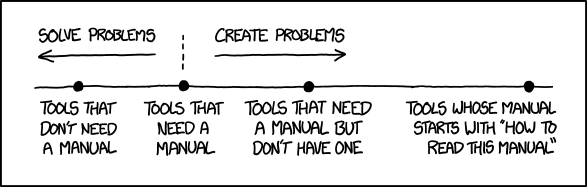
\includegraphics[scale=1]{Graphiques/manuals}
	\caption{\href{http://xkcd.com/}{\copyright\ xkcd}}
	\label{Graphiques_Calvin}
\end{figure}
\end{Verbatim}



  		\subsection{Les chemins sous \LaTeX}

Dans les chemins (noms de fichiers et r�pertoires), \latex ne supporte pas les caract�res sp�ciaux et notamment les blancs. 

Quand vous sp�cifiez le chemin pour un style, une image, un tableau, une partie de document, vous ne pouvez donc pas utiliser de caract�res sp�ciaux accentu�s et de blancs dans les chemins.


  		\subsection{L'inclusion dans un document volumineux}

Vous pouvez inclure du code \latex provenant d'un autre fichier dans un document \LaTeX.

Cela permet, par exemple, de faire un livre avec un fichier par chapitres ou bien de ne pas inclure les tableaux directement dans le corps du document (avec Sweave par exemple).




Pour cela vous disposez de deux commandes \textit{input} et \textit{include}.

La commande \textit{input} ins�re directement le code \latex tandis que la commande \textit{input} ins�re un saut de page avant le contenu du document ins�r�.

Toutefois on ne peut pas imbriquer un appel � un fichier � l'int�rieur d'un autre. On ne pourra donc pas inclure un tableau par un \textit{include} dans un fichier qui sera lui-m�me import� par un autre \textit{include}.


\section{D�finir une fonction personnalis�e}

  		\subsection{D�finir une fonction personnalis�e}
  		
                Pour ins�rer un graphique dans un document de fa�on r�pet�e, autant l'�crire une fois... dans le pr�ambule...

\code
\newcommand{%
\LinuxA}
{
\includegraphics[scale=0.1]
{Graphiques/linux.png}}
\end{Verbatim}


  		
Dans cet exemple, on d�finit une commande \textbackslash Linux qui ajoute une image.

\LinuxA est mon OS pr�f�r�.

Mais on voit qu'il y a un probl�me car le blanc entre le texte et la macro dispara�t.



  		\subsection{xspace}
  		
La m�me fonction avec l'utilisation du package \textit{xspace}.

\code
\newcommand{%
\LinuxB}
{
\includegraphics[scale=0.1]
{Graphiques/linux.png}\xspace}
\end{Verbatim}



\LinuxB est mon OS pr�f�r�.

Le \textbackslash xspace situ� en fin de commande va, lors de la
compilation, v�rifier si un espace est n�cessaire et l'ajouter si
besoin.  


  		\subsection{Avec des arguments}

On aurait pu �crire une fonction plus g�n�rique comme par exemple~:

\code
\newcommand{%
\Image}[2]
{\includegraphics[scale=#1]
{Graphiques/#2}}
\end{Verbatim}

Dans ce cas l'appel est le suivant~:
\code
\Image{0.1}{linux.png}
\end{Verbatim}


  		\subsection{Red�finition d'une fonction existante}

On pourrait vouloir par exemple modifier une fonction existante pour les besoins de la mise en page. La redefinition utilise une syntaxe l�g�rement diff�rente.

La fonction ci-dessous remplace l'italique de la fonction \emph{emph} par des caract�res en gras.
 
\code
\renewcommand{%
\emph}[1]
{\textbf{#1}}
\end{Verbatim}


  		\subsection{Package de programmation}

		Enfin pour faire de la programmation simple, on peut cr�er des variables en \latex et les packages \textit{ifthen} permet de faire des boucles et des tests conditionnels.


  					



\section{Les premiers pas sous Beamer}

  		\subsection{Les paquets pour faire des diapositives}

	Il existe deux paquets pour faire des paquets sous \LaTeX~:
\begin{description}
	\item[prosper] Nous n'en parlerons pas ici
	\item[beamer] c'est le paquet dont je vous parlerais ici
\end{description}
		
	Beamer a �t� utilis� pour faire ces diapositives. Vous pouvez donc regarder les sources des documents pour avoir un exemple plus vivant.


  		\subsection{Dans le pr�ambule...}

	Premi�rement, il faut changer le type du document, au lieu de \emph{article} par exemple il faut mettre~:
\code
\documentclass{beamer}
	\usetheme{Warsaw}
\end{Verbatim}

	La premi�re ligne correspond au type \emph{beamer} qui nous int�resse ici. Le second permet de d�finir le th�me, c'est-�-dire l'apparence de vos diapos. Ce sont des "mod�les" de diapos. Vous pourrez �videmment personnaliser si vous le souhaitez.
		


  		\subsection{Dans le corps du texte...}

Dans le corps du texte, les commandes � utiliser pour d�finir une diapositive sont les suivantes~:
\code
Mon texte...
\end{Verbatim}

	ce qui donne la diapo de la page suivante...


Mon texte...


\section{Titres et organisation}


	Les commandes \emph{\textbackslash section} et \emph{\textbackslash subsection} sont disponibles et vous permettent de structurer votre pr�sentation. 

\vspace{0.1cm}
Certains mod�les utilisent ces informations pour cr�er un affichage de la progression de la pr�sentation.



  		\subsection{Titres des diapositives}

Vous pouvez rajouter des titres aux diapositives. Ces titres seront clairement visibles sur le document mais ne seront pas index�s dans la table des mati�res.

\vspace{0.1cm}
Sur ce mod�le il occupe le bandeau juste au dessus du texte. La syntaxe est relativement simple~:




\code
\subsection{Mon titre}
Mon texte ....
\end{Verbatim}


Mon texte ....


  		\subsection{Titres des diapositives}

La syntaxe ci-dessous est aussi possible... pour le m�me r�sultat.

\code
\subsection
Mon texte ....
\end{Verbatim}



  		\subsection{Ajout de Verbatim}

S'il y a au moins un bloc \emph{listings} ou \emph{verbatim} il faut ajouter une balise pour \LaTeX~:

\code
\subsection{Mon titre}
Mon texte ....
\end{Verbatim}



\section{Mise en page et environnements}

  		\subsection{Ajout de Verbatim}

On ne peut pas utiliser la syntaxe suivante dans cet ordre.

\code
Mon texte ....
\end{Verbatim}



  		\subsection{Options de mise en page suppl�mentaires...}

Beamer offre la possibilit� de mettre tout ou partie du texte en �vidence en utilisant la balise \emph{block}

\code
\subsection{Mon titre}
\begin{block}{Mon titre de bloc}
Mon texte ....
\end{block}
\end{Verbatim}


  		\subsection{Options de mise en page suppl�mentaires...}

Les environnements  suivants sont �galement disponibles...

\begin{itemize}
	\item alertblock
	\item theorem
	\item proof
	\item example
	\item beamercolorbox
\end{itemize}




Comme d'autres logiciels, on peut ins�rer des �tapes~:

\code
\begin{itemize}
	\item<1-> alertblock
	\item<2-> theorem
	\item<3-> proof
	\item<4-> example
	\item<5-> beamercolorbox
\end{itemize}
\end{Verbatim}




Dans le code pr�c�dent, \emph{alertblock} sera visible de la diapo un � la derni�re, \emph{theorem}, de la diapo 2 � la derni�re et ainsi de suite...


\section{Th�mes et sous forme d'article...}

  		\subsection{Les th�mes}

Pour avoir un aper�u des th�mes Beamer, il y a ce \href{http://mcclinews.free.fr/latex/beamergalerie.php}{site }.




  		\subsection{Sortie sous forme d'article}

Pour sortir les diapositives sous la forme d'un article, il suffit de changer le \emph{documentclass}~:

\code
\documentclass{article}
...
\usepackage{beamerarticle}
...
\end{Verbatim}




  					



\section{Ressources pour \latex}

  		\subsection{Ressources}
  		
	\begin{description}
		
		\item[\href{http://www.framabook.org/latex.html}{FramaBook \LaTeX}] 
	
		\item[\href{http://en.wikibooks.org/wiki/LaTeX}{Wikibook \LaTeX}]

		\item[\href{http://vgoulet.act.ulaval.ca/latex/}{Page sur \LaTeX de Vincent Goulet (et Emacs)}]		
		\item[Digital Typography Using \latex] { \scriptsize A. Syropoulos, A. Tsolomitis et N. Sofroniou }

	\end{description}
	

  		\subsection{Ressources suppl�mentaires}

	\begin{description}
	
		\item[\href{http://www.ctan.org/}{Comprehensive \TeX archive Network}] 
	
		\item[\href{http://www.grappa.univ-lille3.fr/FAQ-LaTeX/}{FAQ \LaTeX~universit� de Lille}]
		
		\item[\href{http://www.tex.ac.uk/}{The UK TeX Archive}]

		\item[\href{http://tex.stackexchange.com/}{\TeX Exchange}]

		\item[\href{http://www.math.jussieu.fr/~mpg/latex/docs/}{Cours de Manuel P�gouri�-Gonnard}]

	\end{description}



  		\subsection{Provenances des images}

	\begin{description}
	
		\item[\href{http://xkcd.com/}{xkcd}] 
	
		\item[\href{http://www.le-terrier.net/pingouin/pingouin.html}{Les pingouins de L. L. DeMars}]
		
	\end{description}

  					



\end{document}
